Despite the event selection requirements previously described, the post-selection yields are still dominated by the backgrounds,
and have insufficient statistics to determine the presence of the ttH signal, making further discrimination necessary.
The approach adopted in this search is to split the selected events into several mutually exclusive categories with
different signal to background ratios.
In each of these categories the signal is extracted from the distribution of a suitable discriminating variable.

In order to exploit the topological characteristics and specificities of the ttH signal with respect to the most
dominant backgrounds, the output of the boosted decision tree (BDT), trained using a selection of kinematic
variables, is used as the discriminating variable for the signal extraction.
In this analysis, the samples used for BDT training and evaluation are the ones reported in Sec. \ref{sec:samples}.

Both final states with two same sign leptons (2lss) and at least three leptons ($\geq$=3l) have dominant backgrounds originating
from the \ttbar\ and \ttV\ (V=W/Z) processes. In order to have an efficient discrimination against both of these processes,
a two-dimensional (2D) BDT approach is introduced. For each of the 2lss and $\geq$=3l final states, the BDT is separately trained
against the \ttbar\ and \ttV, selecting a set of kinematic variables that provide the largest separation in each training. The BDT
outputs of the training against these two processes are used to construct the 2D space, effectively a scatter plot of the
two discriminators. The consequent 2D distribution is then partitioned to rectangular sectors and ttH signal and background contributions
of each sector are summed and folded to a one-dimensional histogram. With a
convenient partitioning of the 2D space, the resulting difference of the signal and background shapes is enhanced with respect to the
one-dimensional case, for example against the \ttbar, and that is provided by the training of the additional BDT, against the \ttV\  process.

In the following subsections we detail the definitions of the BDTs used as discriminating variable for the signal extraction
in the 2lss and $\geq$=3l categories. We then describe the criterion to decide the binning of the 2D BDT.
Finally, we detail the precise event subcategorization.

\subsection{2lss event BDT}\label{sec:2lss event BDT}
The training is performed using a relaxed event selection that requires at least two preselected same sign leptons with leading and trailing lepton transverse momentum larger than 25 and 15 GeV, respectively, plus at least four jets in the event of which either two loose selected b-jets or one medium b-tagged jet.

The training against the \ttbar background is performed considering the following input variables:
\begin{itemize}
\item maximum absolute pseudorapidity of the two leading leptons
\item multiplicity of hadronic jets
\item minimum distance between the leading lepton and closest jet
\item minimum distance of the trailing lepton and closest jet
%\item missing transverse energy
%\item average separation between the two jets and the transverse mass of the leading lepton 
\item transverse mass of the leading lepton and missing transverse energy
\item hadronic top reconstruction (score of the discriminator for best permutation)
\end{itemize}

The training against the \ttV\  background is performed considering the following input variables:
\begin{itemize}
\item maximum absolute pseudorapidity of the two leading leptons
\item multiplicity of hadronic jets
\item minimum distance between the leading lepton and closest jet
\item minimum distance of the trailing lepton and closest jet
\item transverse mass of the leading lepton and missing transverse energy
\item leading lepton transverse momentum 
\item trailing lepton transverse momentum
%\item HT, defined as the scalar sum of the pT of the selected leptons, jets, and the met
\item Hj tagger score after hadronic top jets triplet removal (best permutation)
%\item Hj and Hjj taggers after hadronic top jets triplet removal
\end{itemize}

%The variables listed above are the same used in the previous versions of the analyses,
%with the exception of HT, which is now used in the training against \ttV\, and the last-itemized for both trainings.
The sets of observables listed above include new variables that have not been used before, such as the 
score of the hadronic top reconstruction and the Hj tagger, which are explained in more detail below.
The aforementioned hadronic top jet triplet, when using the Hj tagger in the training against the \ttV\ background,
indicates a triplet of jets with the highest likelihood to orginate from hadronic top decay in 2lss events.
This jet triplet is found through the event reconstruction BDT explained below, whose score is used as an input in the training against \ttbar.
The Hj tagger, described more in detail in the following,
is an algorithms designed to identify jets originating from one of the W of the Higgs in 2lss events.
The Higgs jets search is performed against all the jets that enter the 2lss region, except those forming a triplet compatible
with an hadronic top decay (from which the expression hadronic top jets triplet removal).

\subsubsection{Hadronic top reconstruction}
The reconstruction of the hadronic top decay is performed with a BDT. The objective is to correctly match
each selected jet and lepton to a final state particle in a $t\bar{t}H$ event, then
use the BDT response and other variables from the reconstruction to discriminate
against events without a hadronic top.     

Event reconstruction targets the 2lss category, specifically where the Higgs decays
to $W$ bosons. In the 2lss category, this means that one lepton originates from the
top system, and the other from the Higgs. For the jets, one of the
$W$ bosons from the Higgs decays hadronically, one of the top quarks decays
hadronically, producing a total of two b-jets, and four light-flavor jets
from the hadronic $W$ decays.   

{\bfseries Training}

The event reconstruction BDT is trained using the $t\bar{t}H$ monte-carlo powheg
signal sample described previously. 

The signal is correctly matched $t\bar{t}H$ events, which pass the 2lss selection.
Because the 2lss event selection requires at least four jets, the vast majority of signal
events used for training are only partially reconstructed, since a full reconstruction
necessitates six matched jets. Because so few events can be fully reconstructed, we must
consider partial reconstructions for events that have fewer than six matched jets.
The strategy for this is to use 'null' jets whose four-vectors are set to zero to
substitute missing jets in the event. Finally we require the signal events to have two
correctly matched selected leptons, and at least four correctly matched selected jets.

The background consists of all jet and lepton permutations of incorrectly matched
$t\bar{t}$ events. For the background, the null jets are added according to the
jet multiiplicity. For events with seven or fewer selected jets, three null jets are
added, for events with eight selected jets, two null jets are added, and one null jet
is added for events with greater than eight selected jets. To reduce the computation
time and improve performance,
several cuts are applied at each permutation to remove unlikely reconstructions.
These cuts include applying the b-tag requirement on the two jets being considered
as b-jets (1 b-tight, 2 b-loose) described earlier, requiring that no
reconstructed $W$ have a mass greater than 120 GeV, requiring the leptonic top mass
be less than 180 GeV, and requiring 
the hadronic top mass be less than 220 GeV. Additionally, we ignore permutations
arising from swapping two light flavor jets from the same $W$ boson, as the reconstruction is
identical. 

The BDT uses eight input variables, consisting of the CSV of the b-jets from the top
system, the transverse
momentum of the reconstructed hadronic top, the mass of the reconstructed hadronic top,
the mass of the $W$ originating from the hadronic top, the transverse momentum ratio
of lepton from the Higgs with the lepton from the top, and the solid angles between
the lepton from the top and
each b-jet from the top system, and between the lepton from the Higgs.
This approach focuses on the hadronic top decay, as the other aspects of the event
are more difficult to reconstruct due to the missing energy from the neutrinos. 

{\bfseries Evaluation}

The event reconstruction BDT is evaluated by iterating over all possible lepton and jet
permutations, and selecting the highest scoring permutation as the reconstruction for
each event. For the evaluation and usage, the null jet prescription and permutation
cuts used are identical to the background training.
The reconstruction is designed identify events that have a hadronic top present and thus offers
some discrimination against the semi-leptonic $t\bar{t}$ background, shown below in
Figure~\ref{reconstruction:outputVars}.


\begin{figure}[htb]
 \centering
   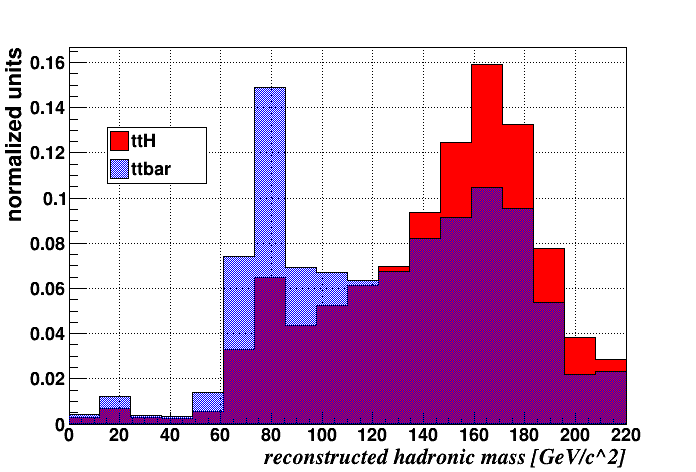
\includegraphics[width=0.4\textwidth]{plots_reconstruction/had_top_mass.png}
   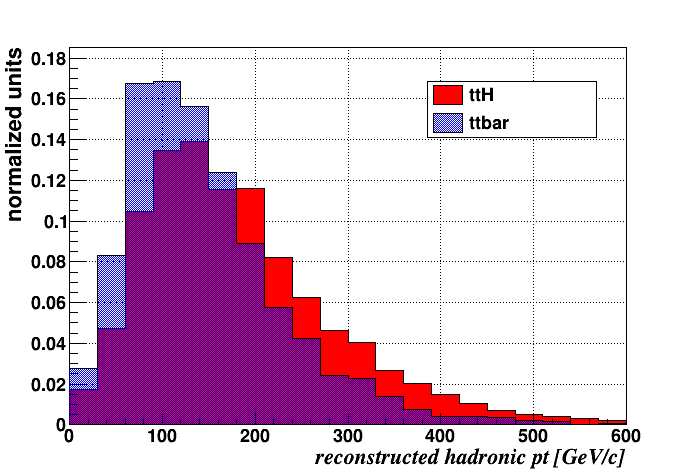
\includegraphics[width=0.4\textwidth]{plots_reconstruction/had_top_pt.png}\\
   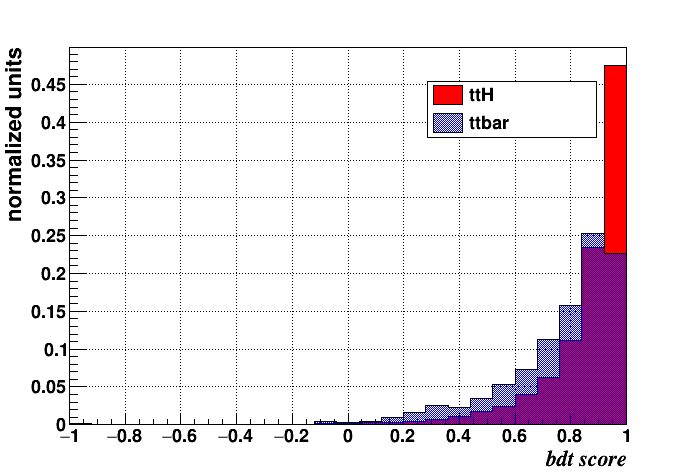
\includegraphics[width=0.4\textwidth]{plots_reconstruction/bdt_score.png}
   \caption{Best BDT score and associated quantities from hadronic top reconstruction.}
  \label{reconstruction:outputVars}
\end{figure}

%% \begin{figure}[htb]
%%  \centering
%%    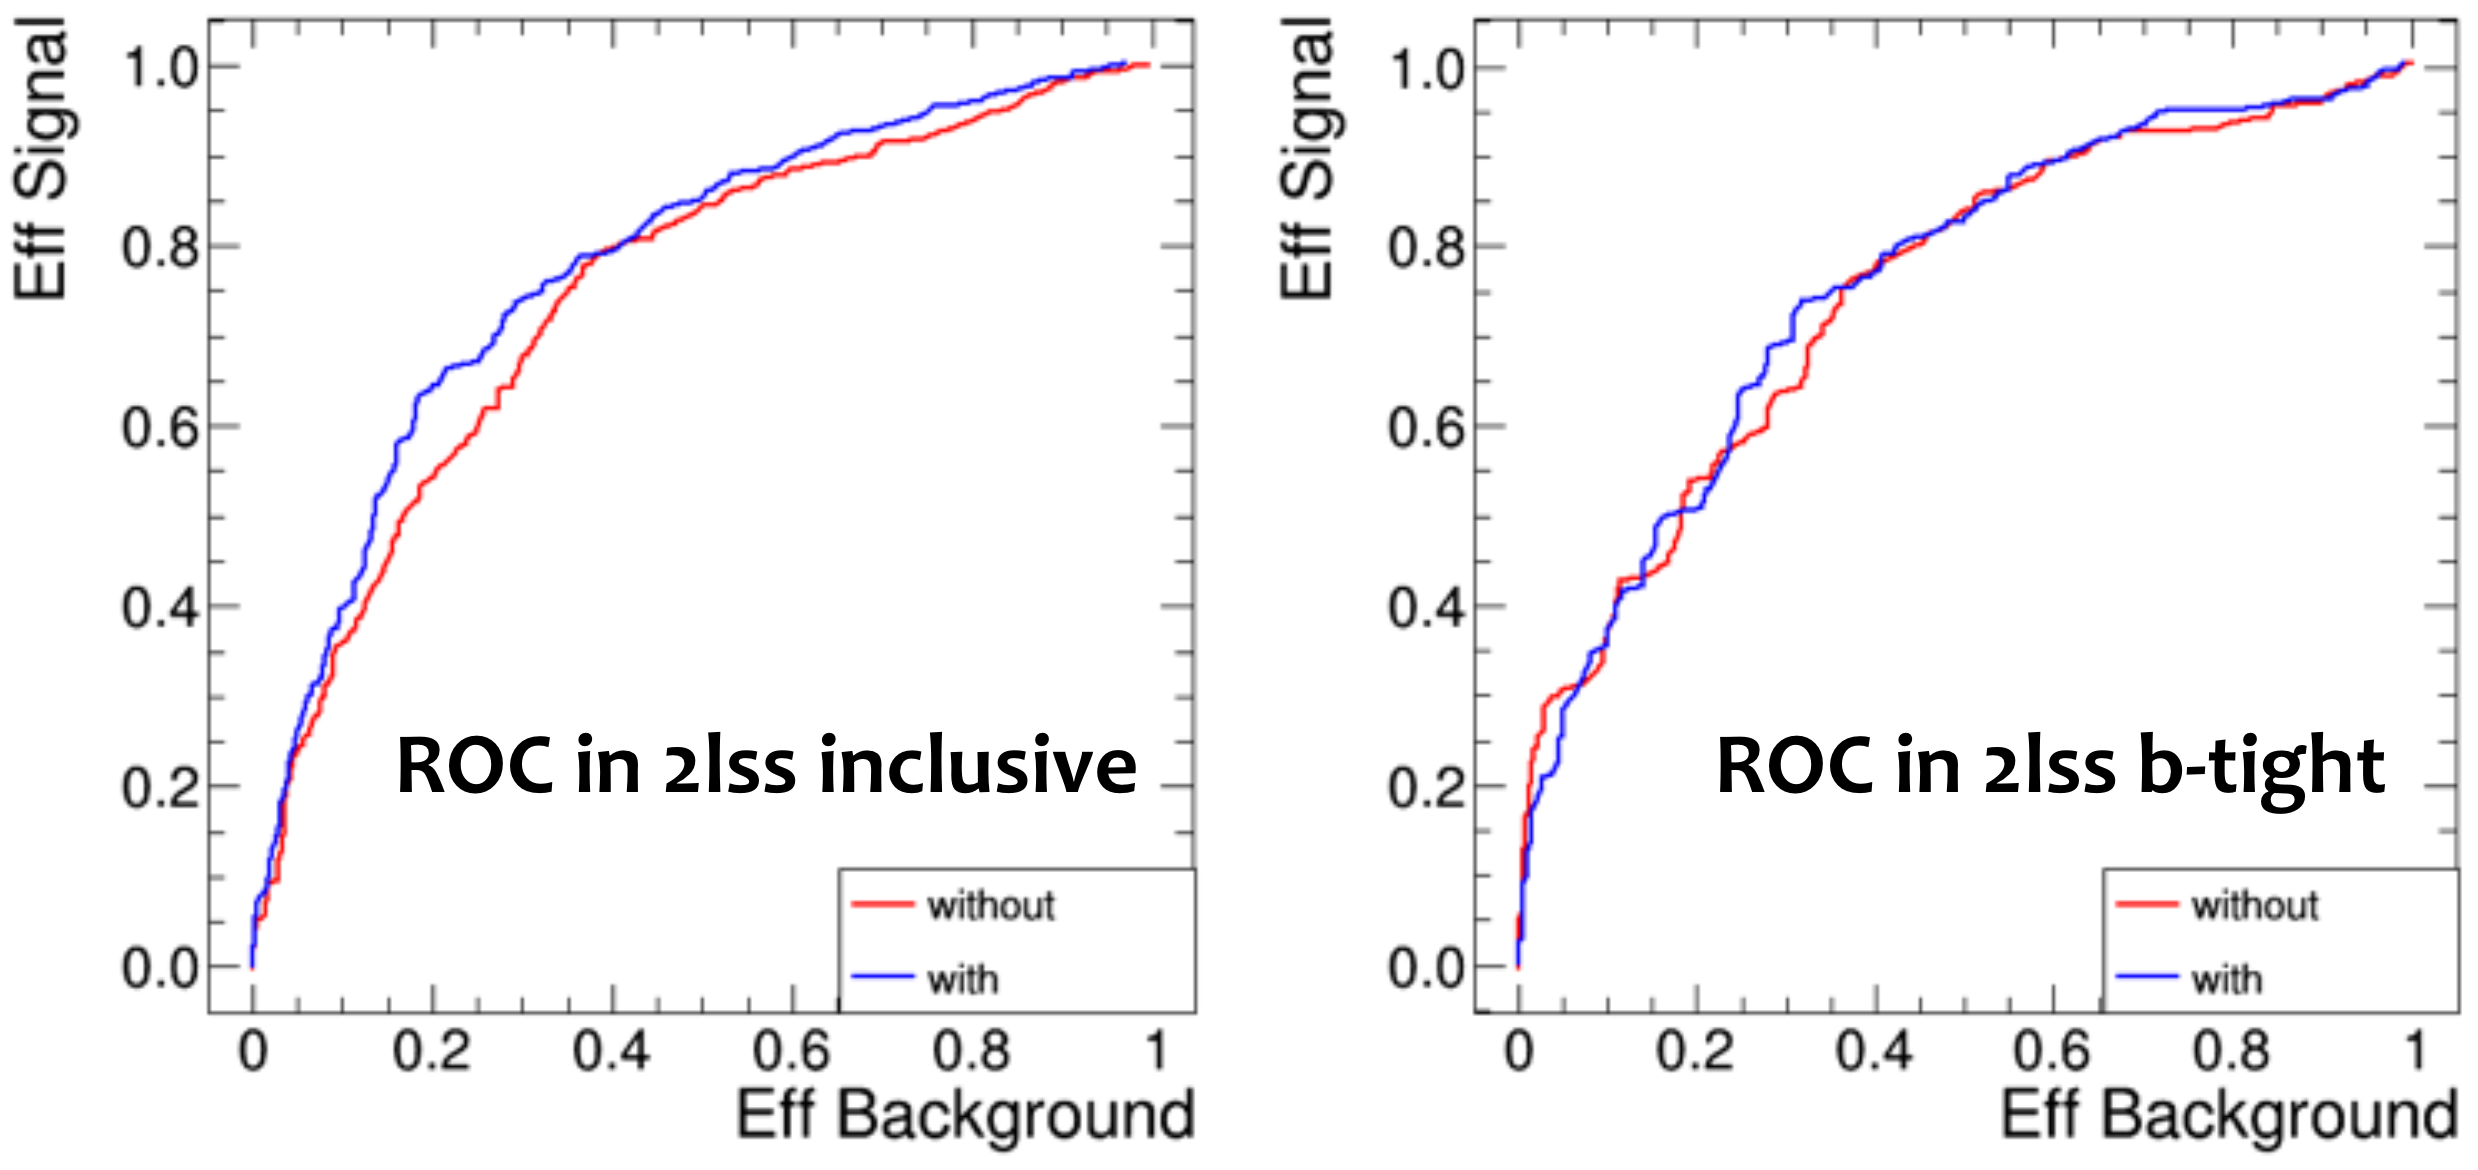
\includegraphics[width=0.7\textwidth]{plots_reconstruction/roc_improvement.png}
%%    \caption{ROC curve of signal extraction BDT with and without reconstruction variables evaluated against $t\bar{t}$.}
%%   \label{reconstruction:roc}
%% \end{figure}


%% \begin{figure}[htb]
%%  \centering
%%    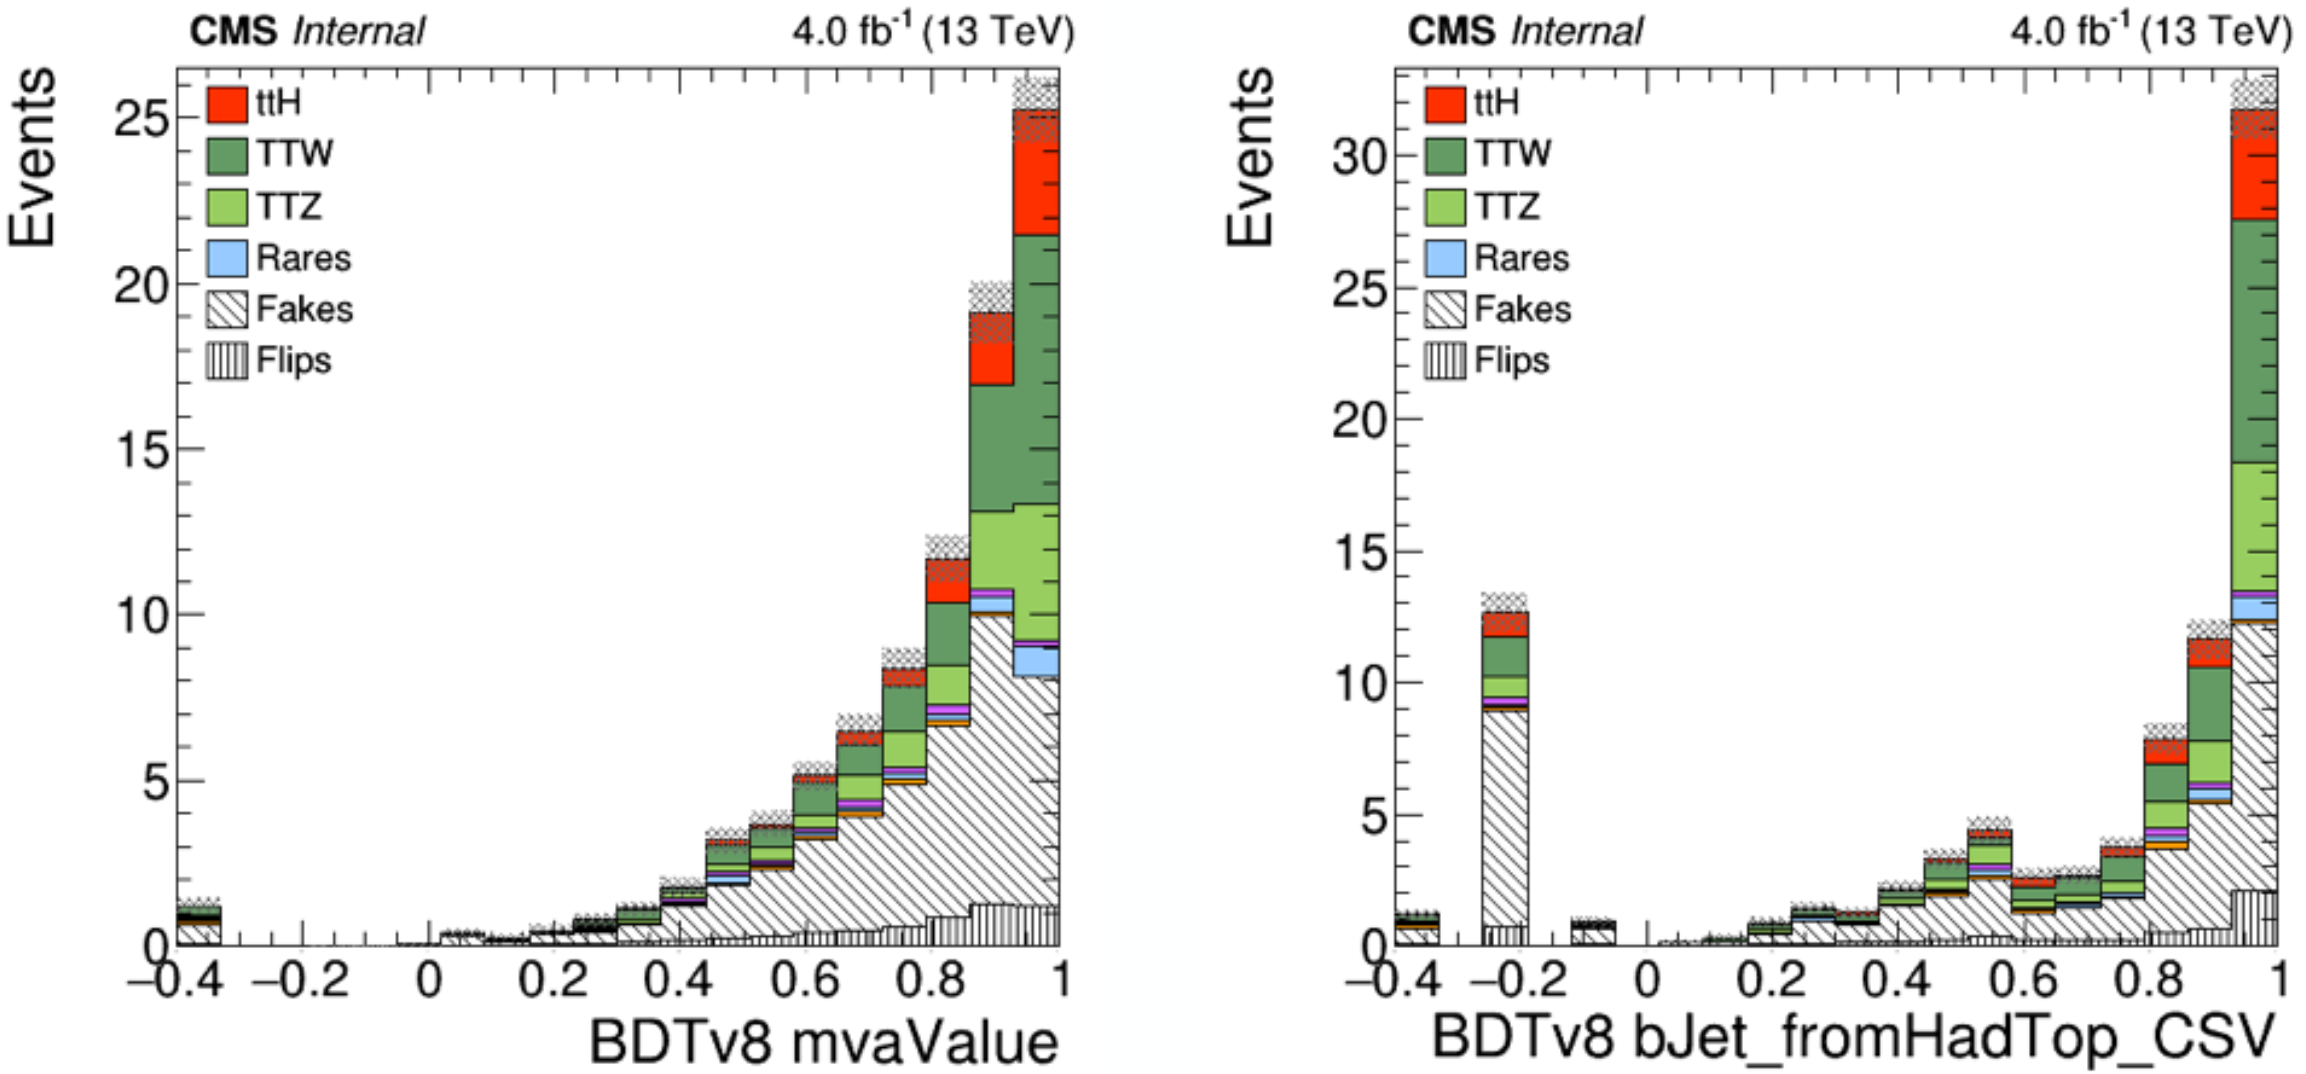
\includegraphics[width=0.7\textwidth]{plots_reconstruction/reconstruction_mva_csv_signal_region.png}
%%    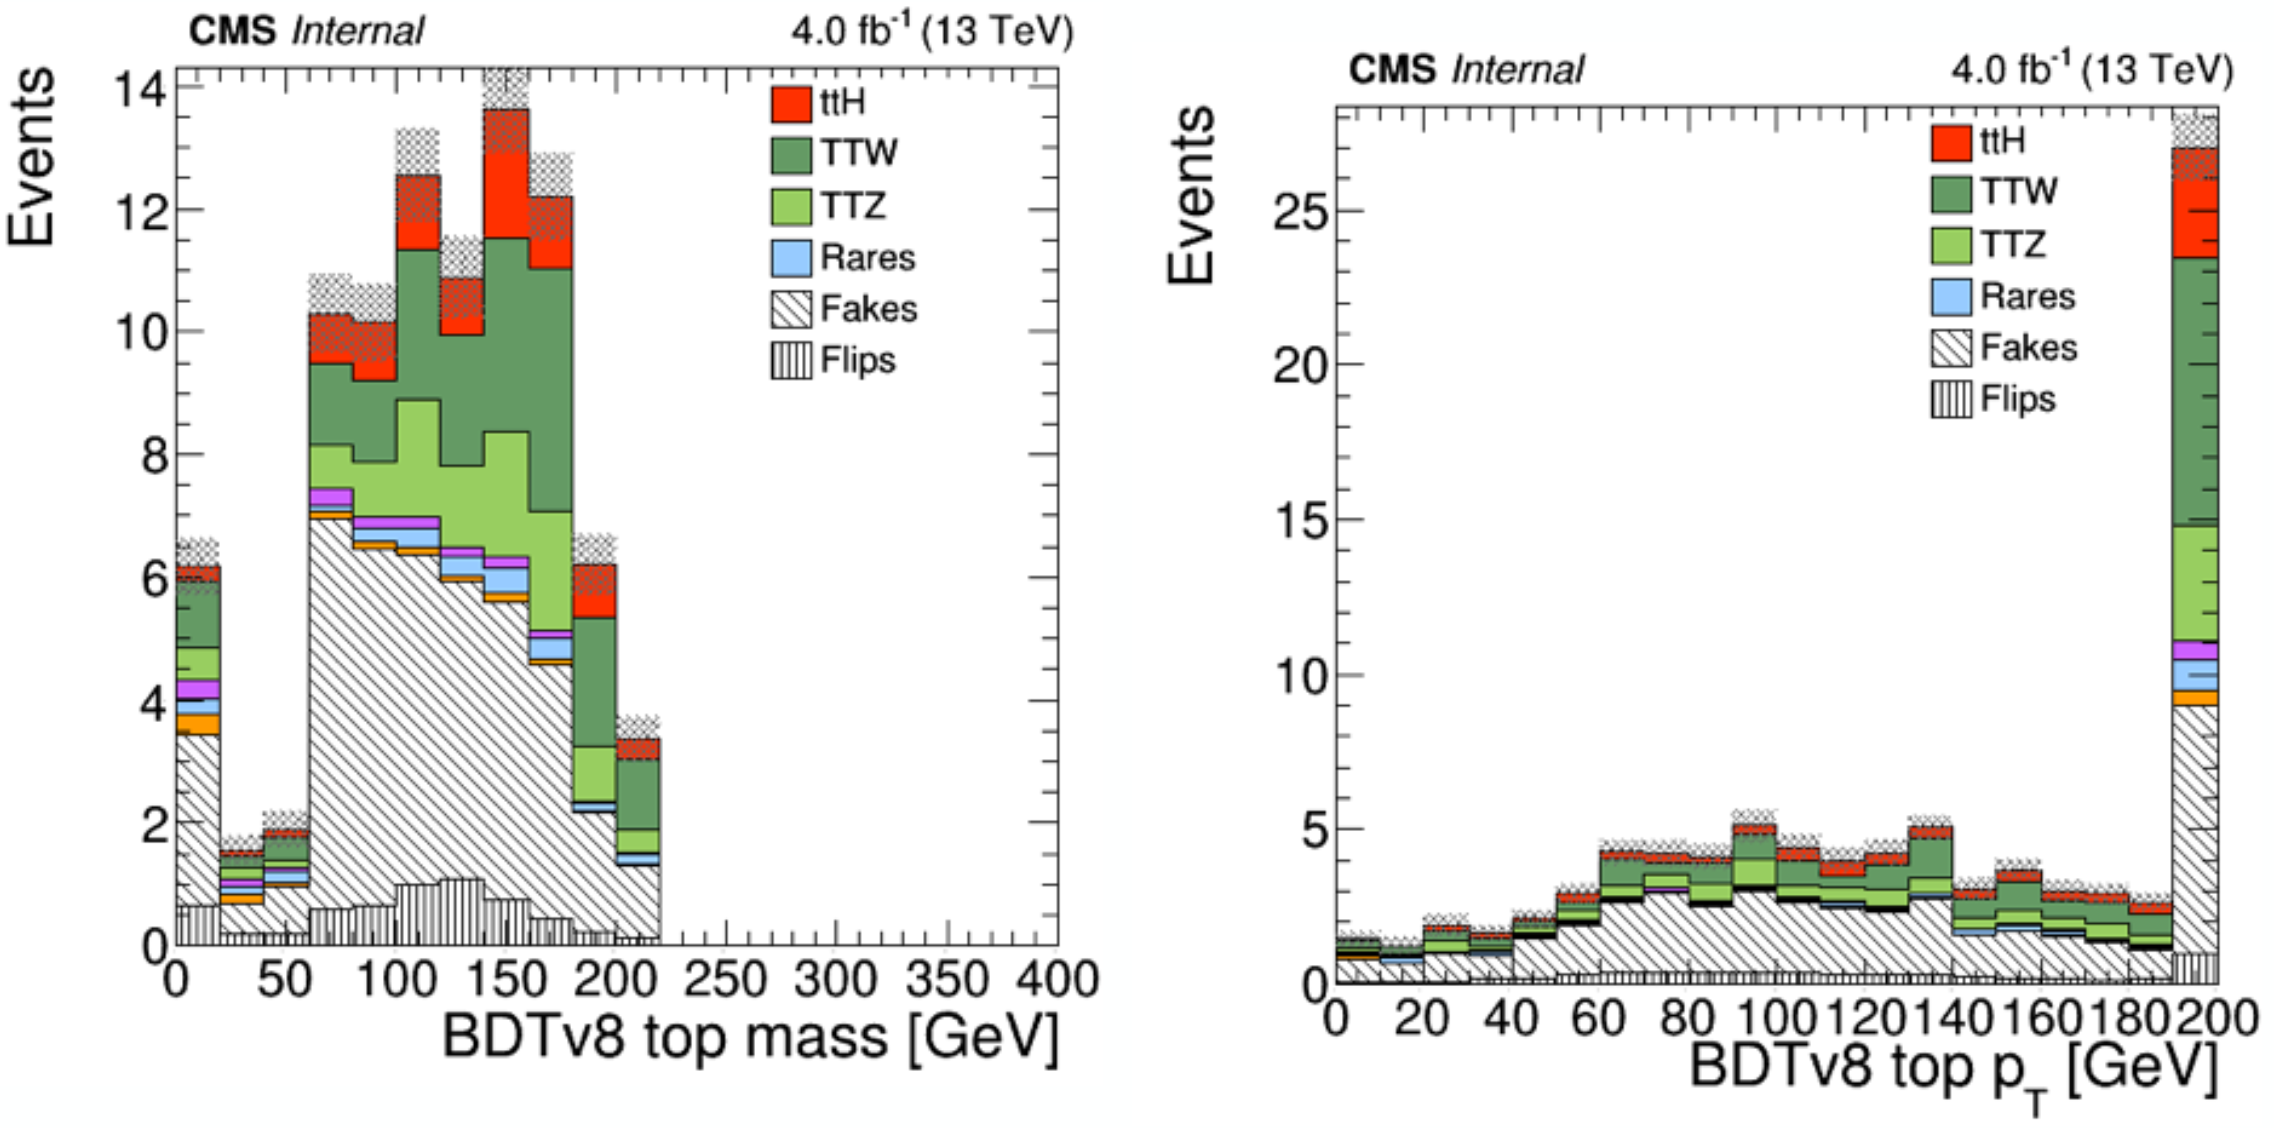
\includegraphics[width=0.7\textwidth]{plots_reconstruction/reconstruction_topmass_toppt_signal_region.png}
%%    \caption{Event reconstruction variables in the 2lss signal region.}
%%   \label{reconstruction:vars_signal_region}
%% \end{figure}

%% \begin{figure}[htb]
%%  \centering
%%    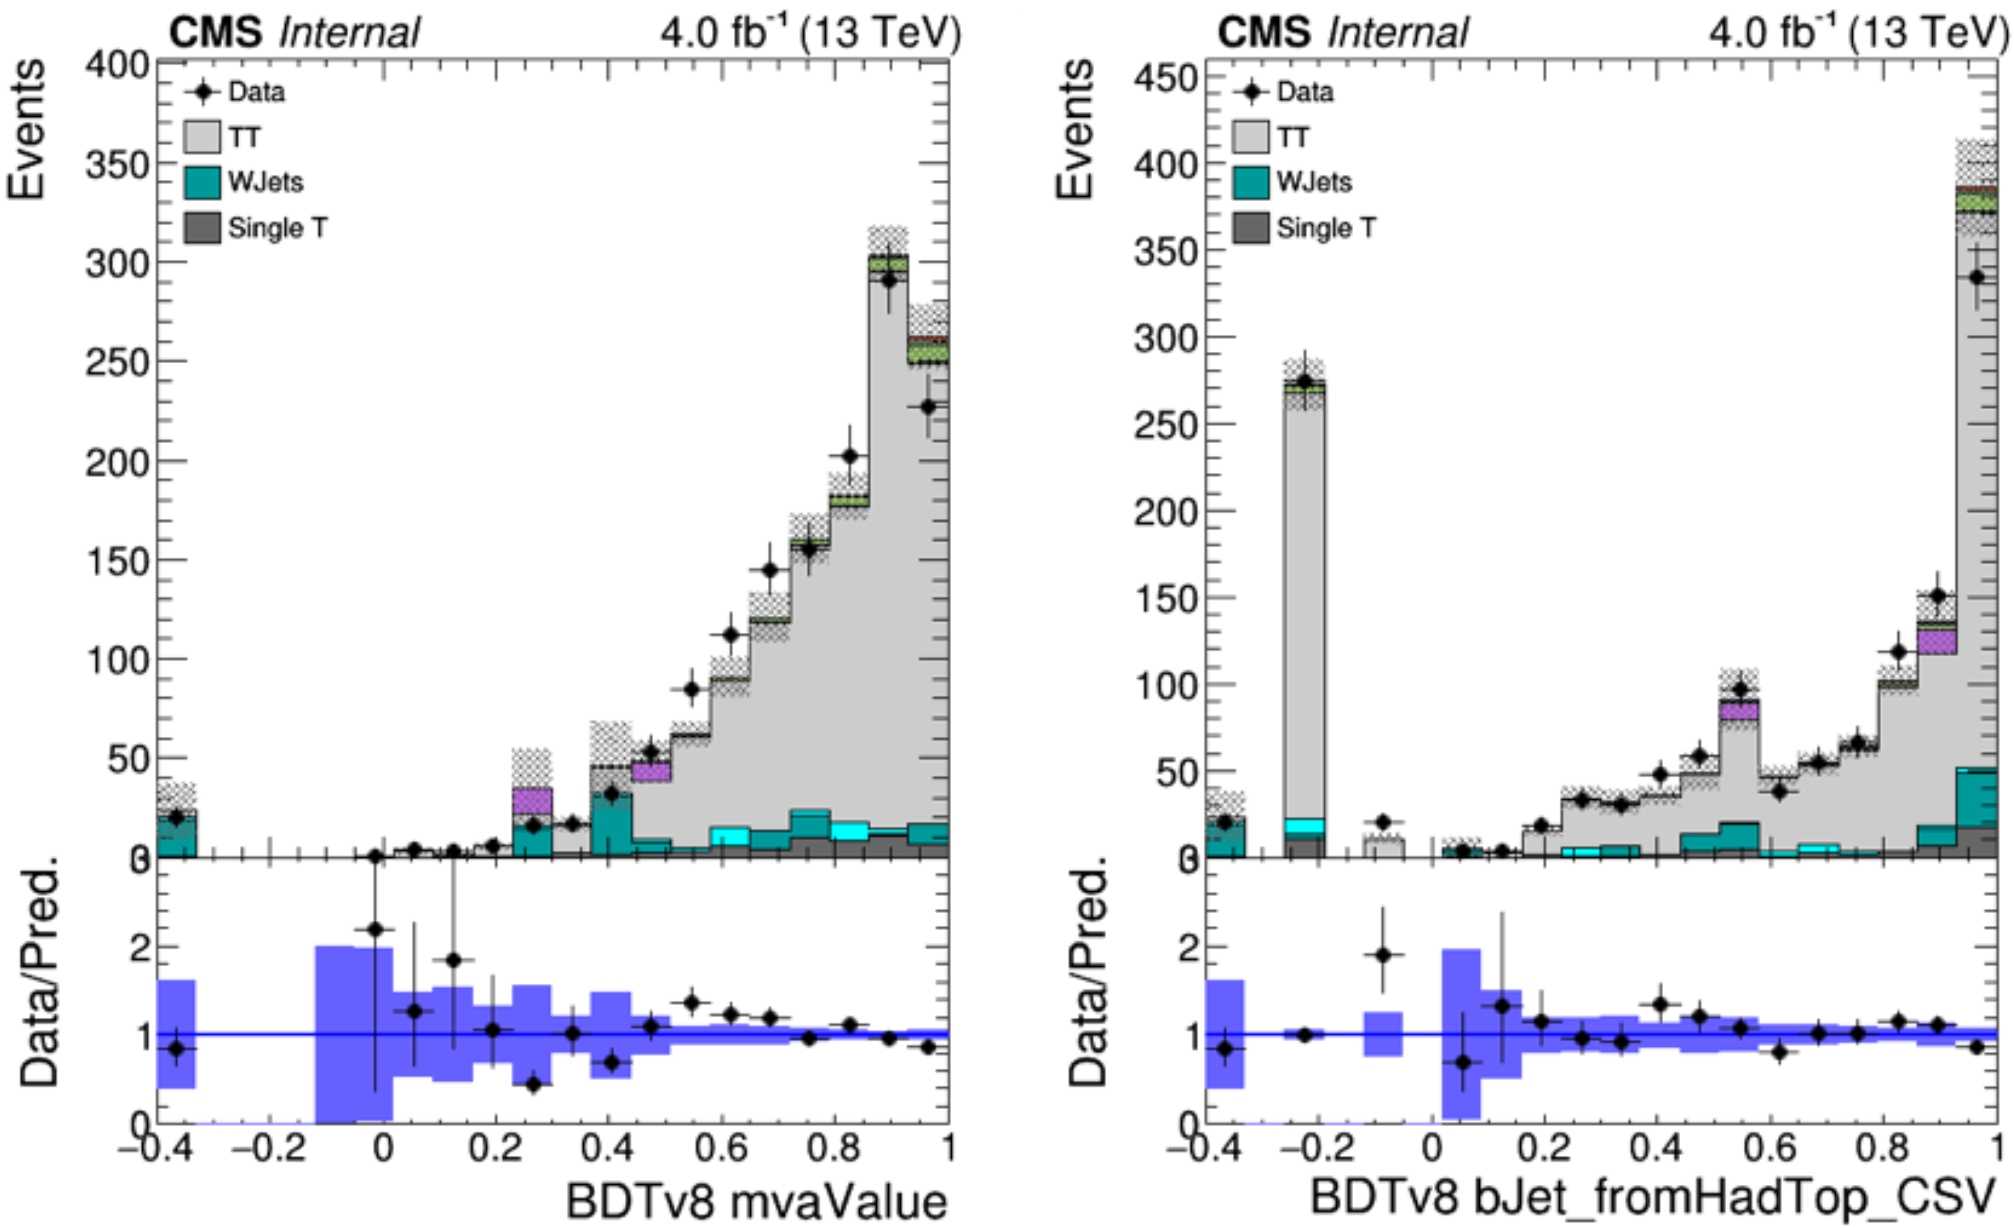
\includegraphics[width=0.7\textwidth]{plots_reconstruction/reconstruction_mva_csv_application_region.png}
%%    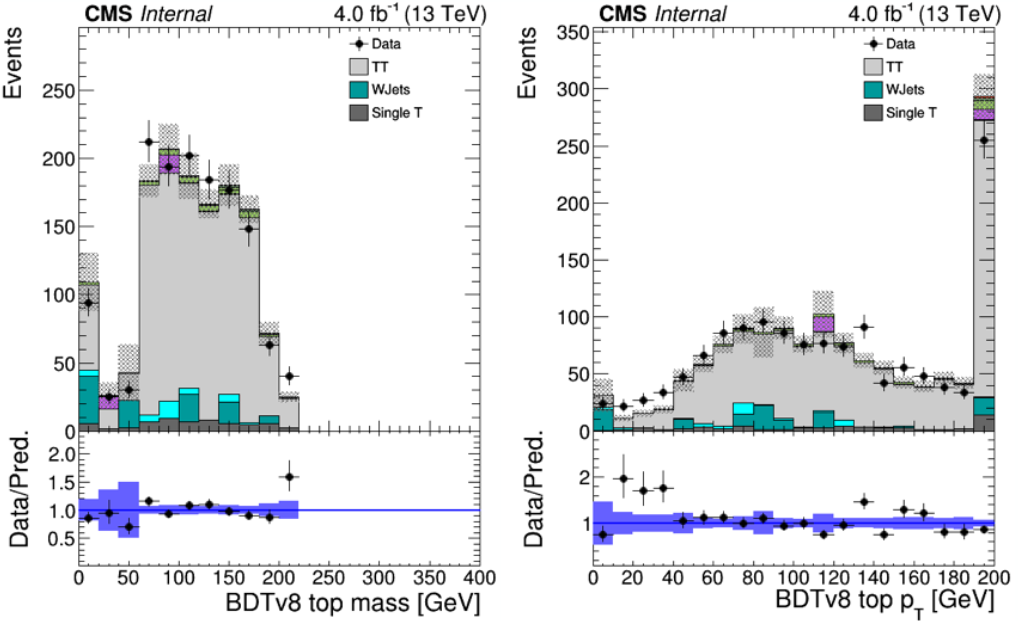
\includegraphics[width=0.7\textwidth]{plots_reconstruction/reconstruction_topmass_toppt_application_region.png}
%%    \caption{Event reconstruction variables in the 2lss application region.}
%%   \label{reconstruction:vars_application_region}
%% \end{figure}

%% \begin{figure}[htb]
%%  \centering
%%    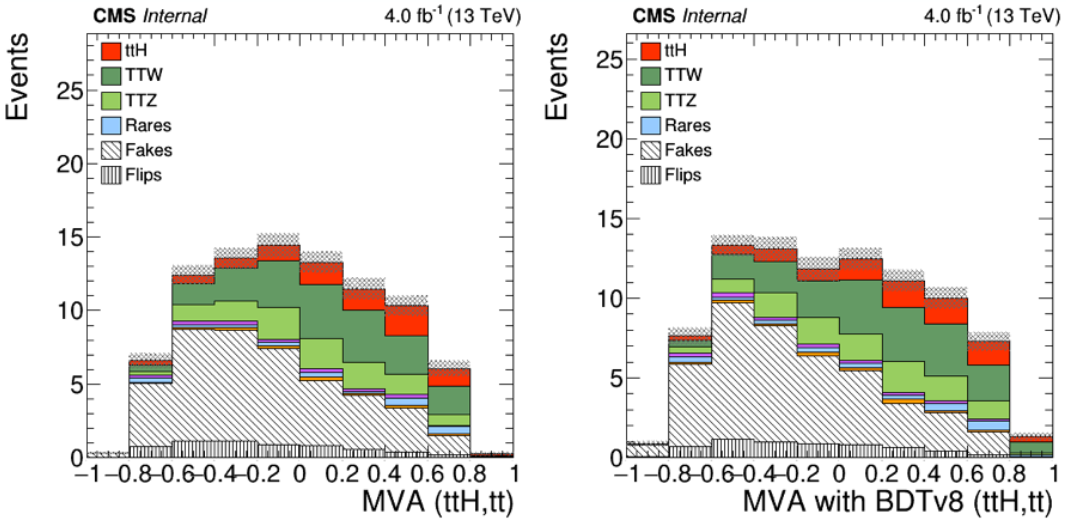
\includegraphics[width=0.7\textwidth]{plots_reconstruction/reconstruction_extraction_mva_output.png}
%%    \caption{Signal extraction MVA output with and with out signal extraction.}
%%   \label{reconstruction:extraction_output}
%% \end{figure}

\clearpage
\subsubsection{The Hj tagger}\label{sec:Hjtagger}
In this section we describe a discriminator aiming at identifying jets that originates from a Higgs decaying to two Ws.
In particular, we target the 2lss category in which the ttH signal decays, in the highest fraction of events, according to the following chain:
$$(t) (t) (H) \rightarrow  (bW) (bW) (WW^*) \rightarrow (bjj)  (b\ell\nu_{\ell}) (\ell\nu_{\ell}jj)$$
We therefore expect 2 b quark jets, 4 jets, 2 same-sign leptons, and missing energy in the final state,
altough, in order to increase the signal acceptance, the analysis requires the presence of at least 4 jets overall.
This means that the Higgs jets do not necessarily enter the signal region.

In order to deal with both the complicated jet combinatoric and the possibility that not all the jets originating from Higgs are selected,
one discriminator is developed: the Higgs-jet (Hj) tagger.
The Hj tagger is an object discriminator that exploits jet identification and kinematic properties
in order to assess the likelihood of a jet of originating in the decay $H \rightarrow WW^* \rightarrow \ell\nu_{\ell}jj$.

The discriminator is developed considering the BDT  multivariate technique.
We rely on the powheg ttH sample and ttV sample to define the signal and the background in the training.
For the Hj tagger the signal is represented by reconstructed jets that are matched at gen-level to jets
of the process $H \rightarrow WW^* \rightarrow \ell\nu_{\ell}jj$, while the background is given by the reconstructed jets in ttV events. 
For the training, we consider the phase space of events that enter the 2lss category, with 0 $\tau_h$.

In the following subsection we list the variables used for the Hj taggers and their expected BDT distributions.

{\bfseries Hj variables and performances}\\
The variables used for the Hj tagger are:
\begin{itemize}
\item minimum dR of the jet and one of the lepton
\item maximum dR of the jet and one of the lepton
\item jet pT
\item jet b-tagging discriminator
\item jet quark-gluon discriminator
\end{itemize}

The performances of the Hj tagger are illustrated in Fig. \ref{fig:HjDistrROC}.
The ROC curve (Fig. \ref{fig:HjDistrROC}, right) highlights the improvement
in performance of the Moriond 2017 BDT (red line) versus the ICHEP 2016 BDT (black line).

\begin{figure}[htb]
 \centering
   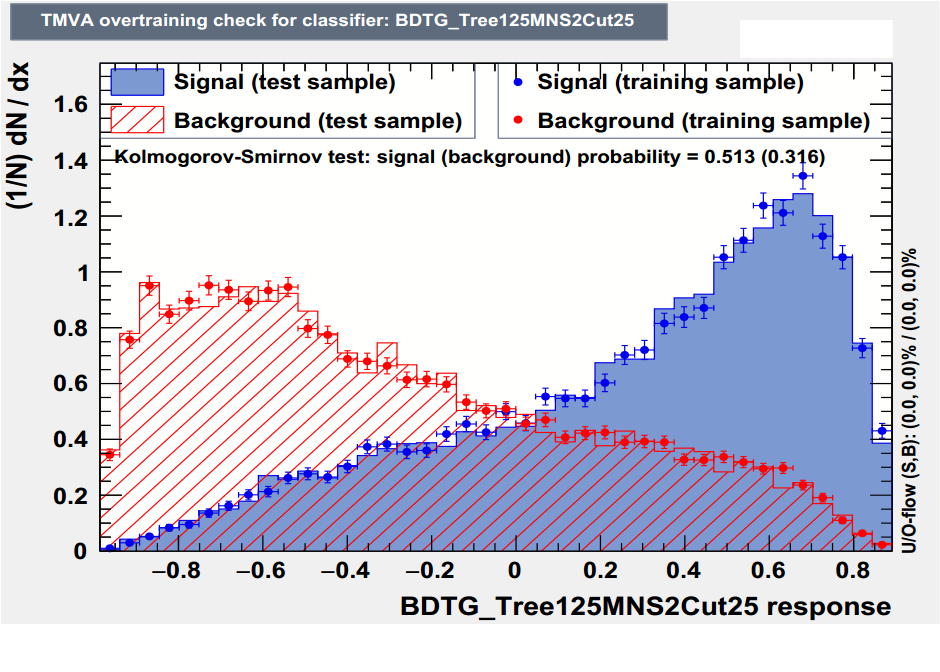
\includegraphics[width=0.48\textwidth]{plots_HjHjj/Jtagger_Ks_.png}
   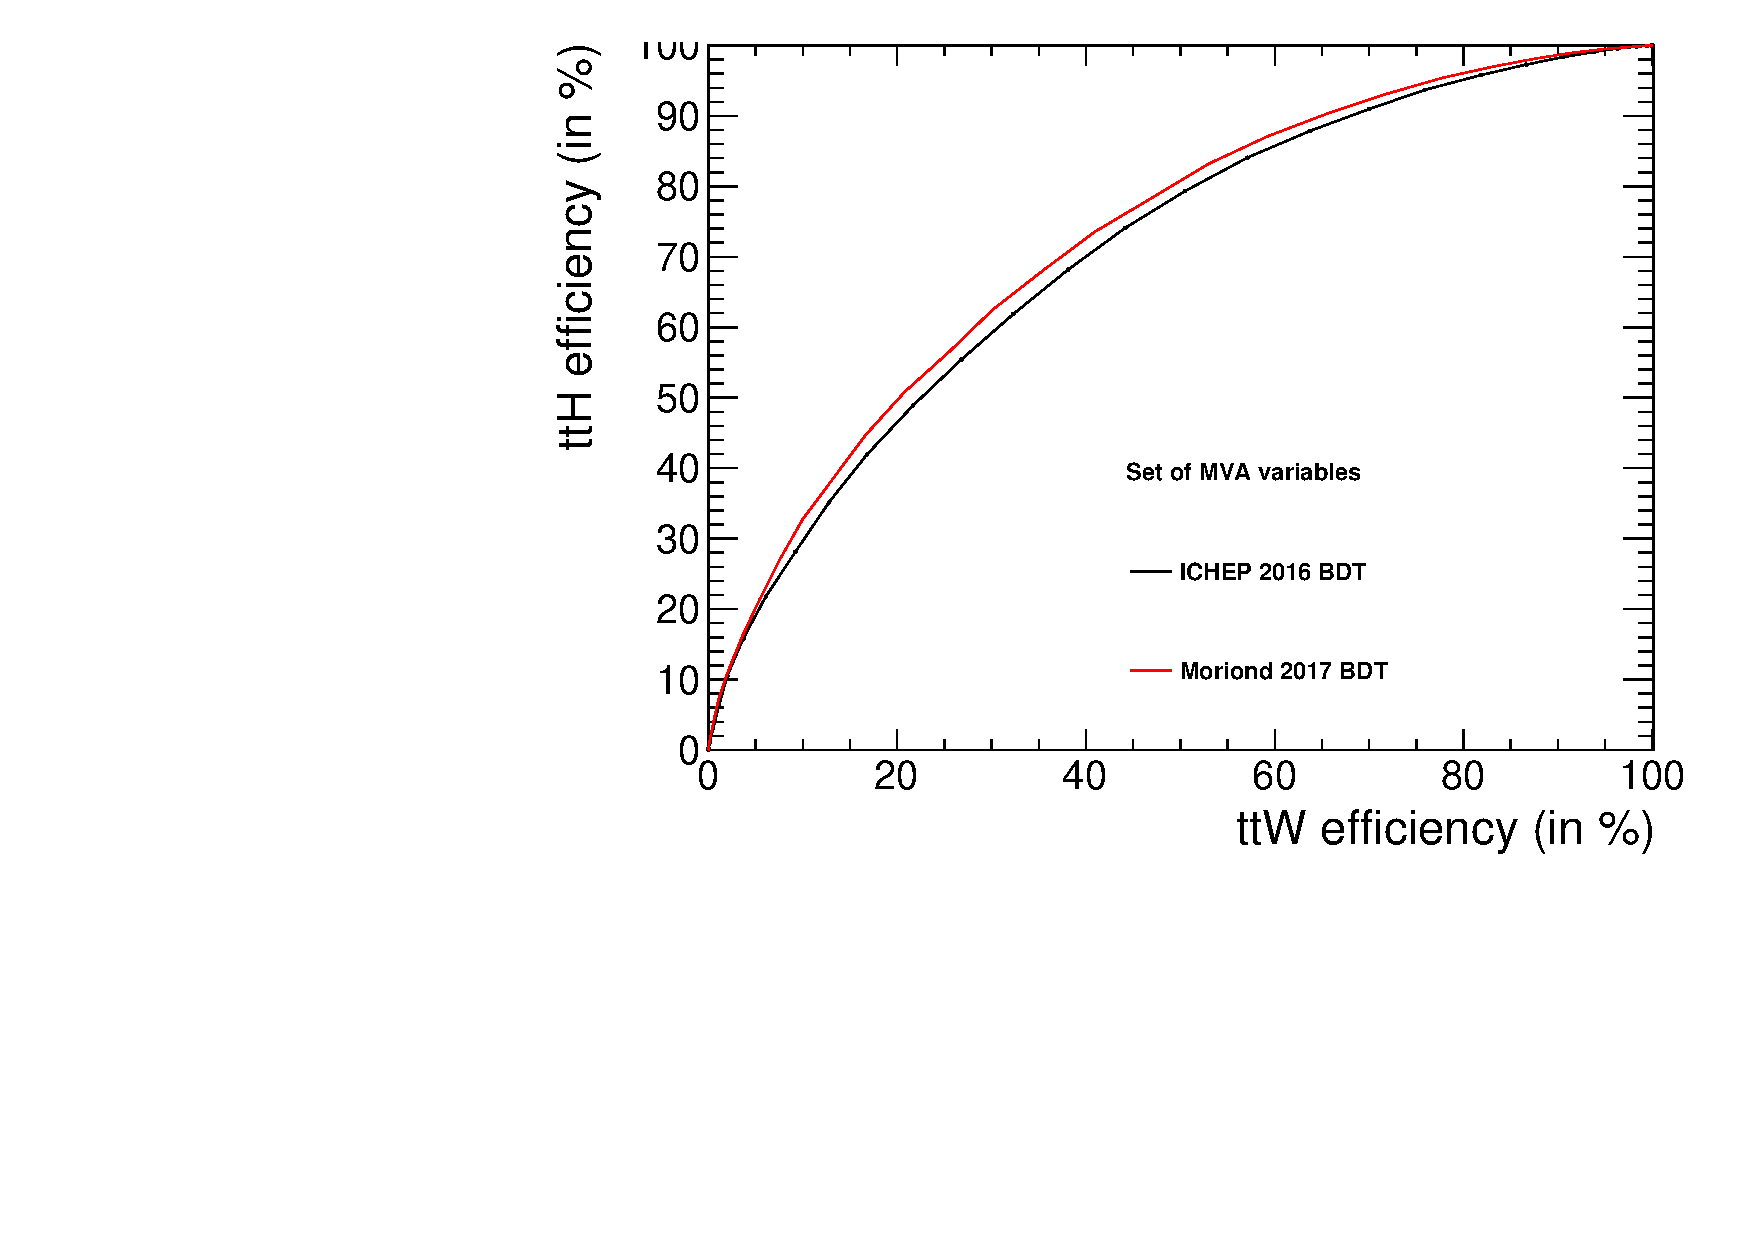
\includegraphics[width=0.48\textwidth]{plots_HjHjj/Roc_Comparison_18Feb.pdf}
   \caption{The Hj distribution (left) and ROC (right). The ROC curve highlights the improvement in performance of the Moriond 2017 BDT (red line) versus            the ICHEP 2016 BDT (black line). Signal and background composition are described in the text.}
   %\caption{The Hj ROC. Signal and background composition are described in the text.}
  \label{fig:HjDistrROC}
\end{figure}

Figures~\ref{fig:2lss_training_1} and \ref{fig:2lss_training_2} show a comparison of the simulated signal (ttH) and background (\ttbar\ or \ttV) processes for each of the input variables to the BDT discriminator.
Figure ~\ref{fig:2l_mvaTraining} shows the separation power of the BDT discriminators.
%while Figures~\ref{fig:2l_mvaOutput} shows the distributions of these discriminators.

\begin{figure}[htb]
        \centering
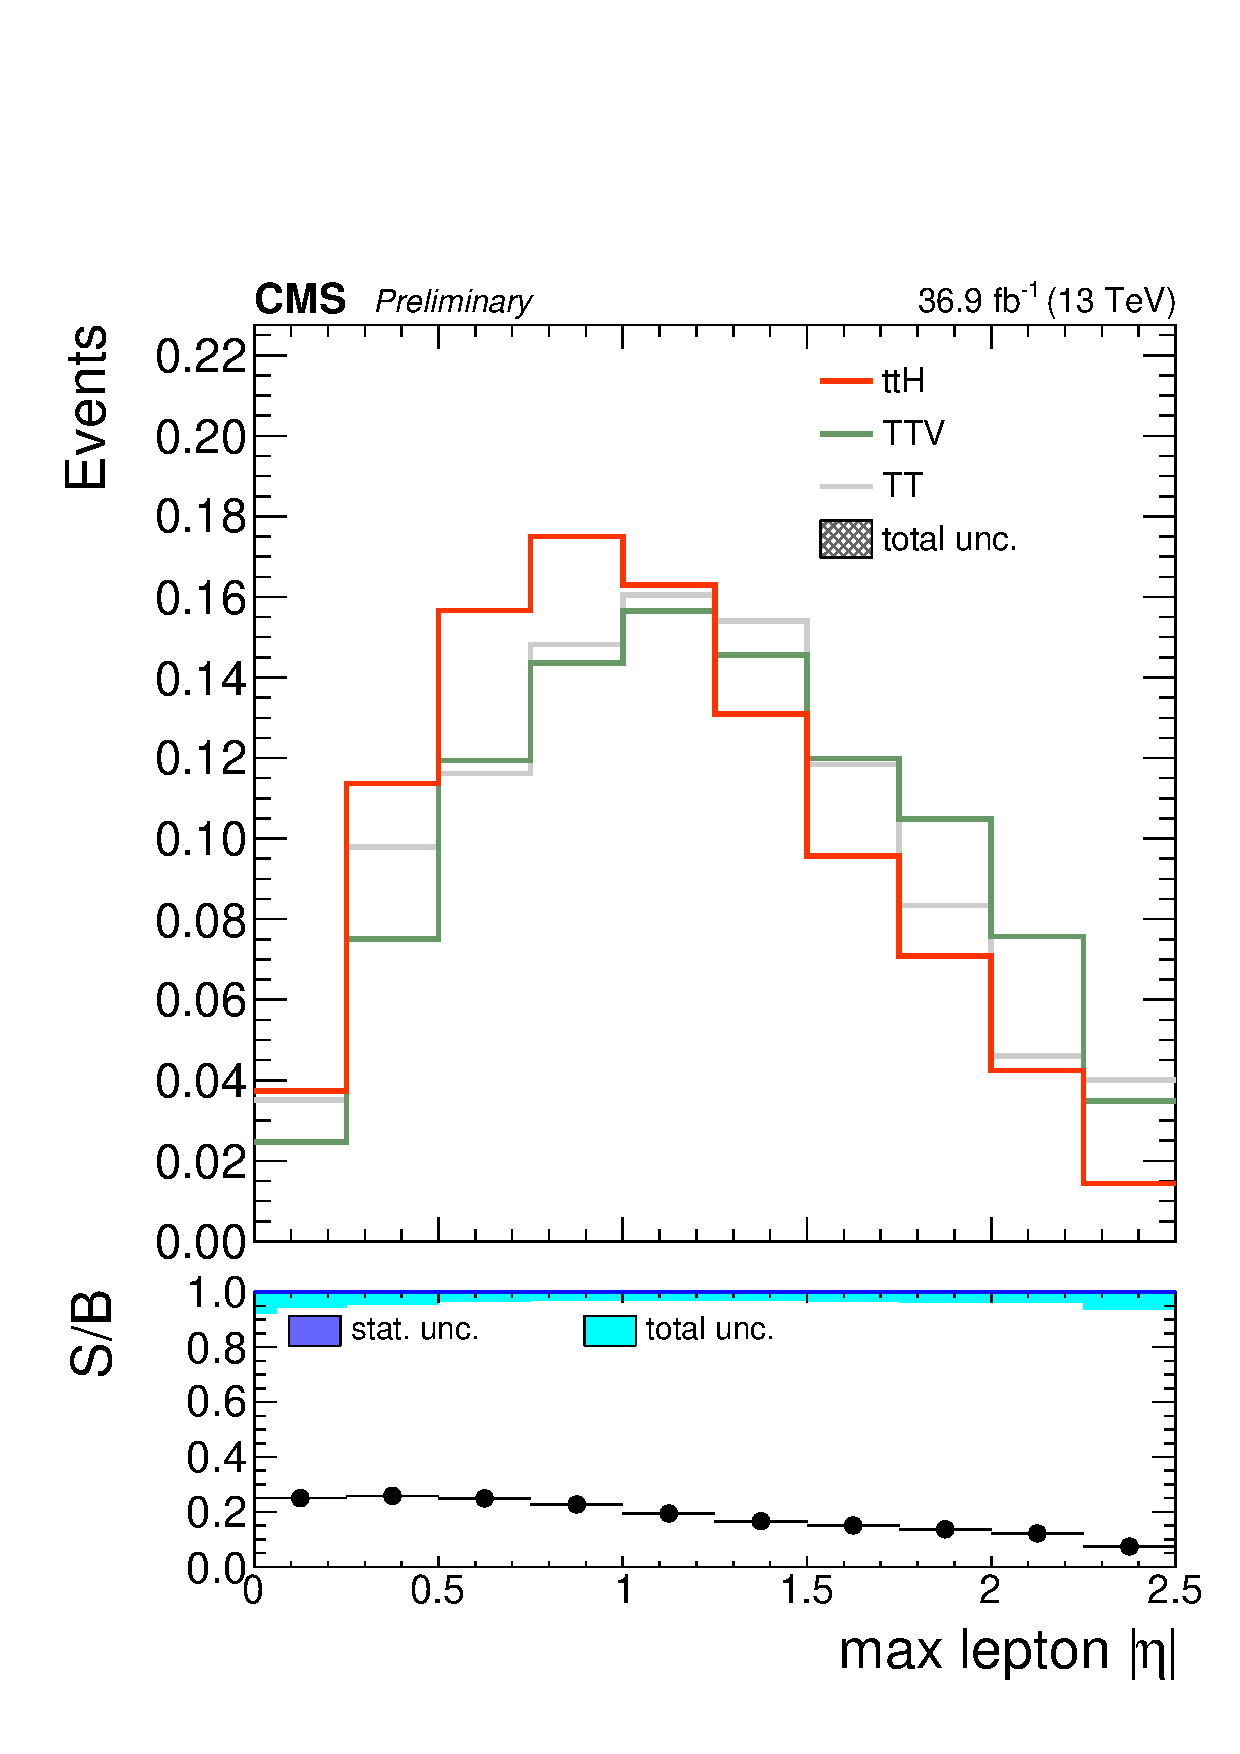
\includegraphics[width=0.32\textwidth]{plots_extraction/training/2lss/kinMVA_input_max_Lep_eta.pdf}
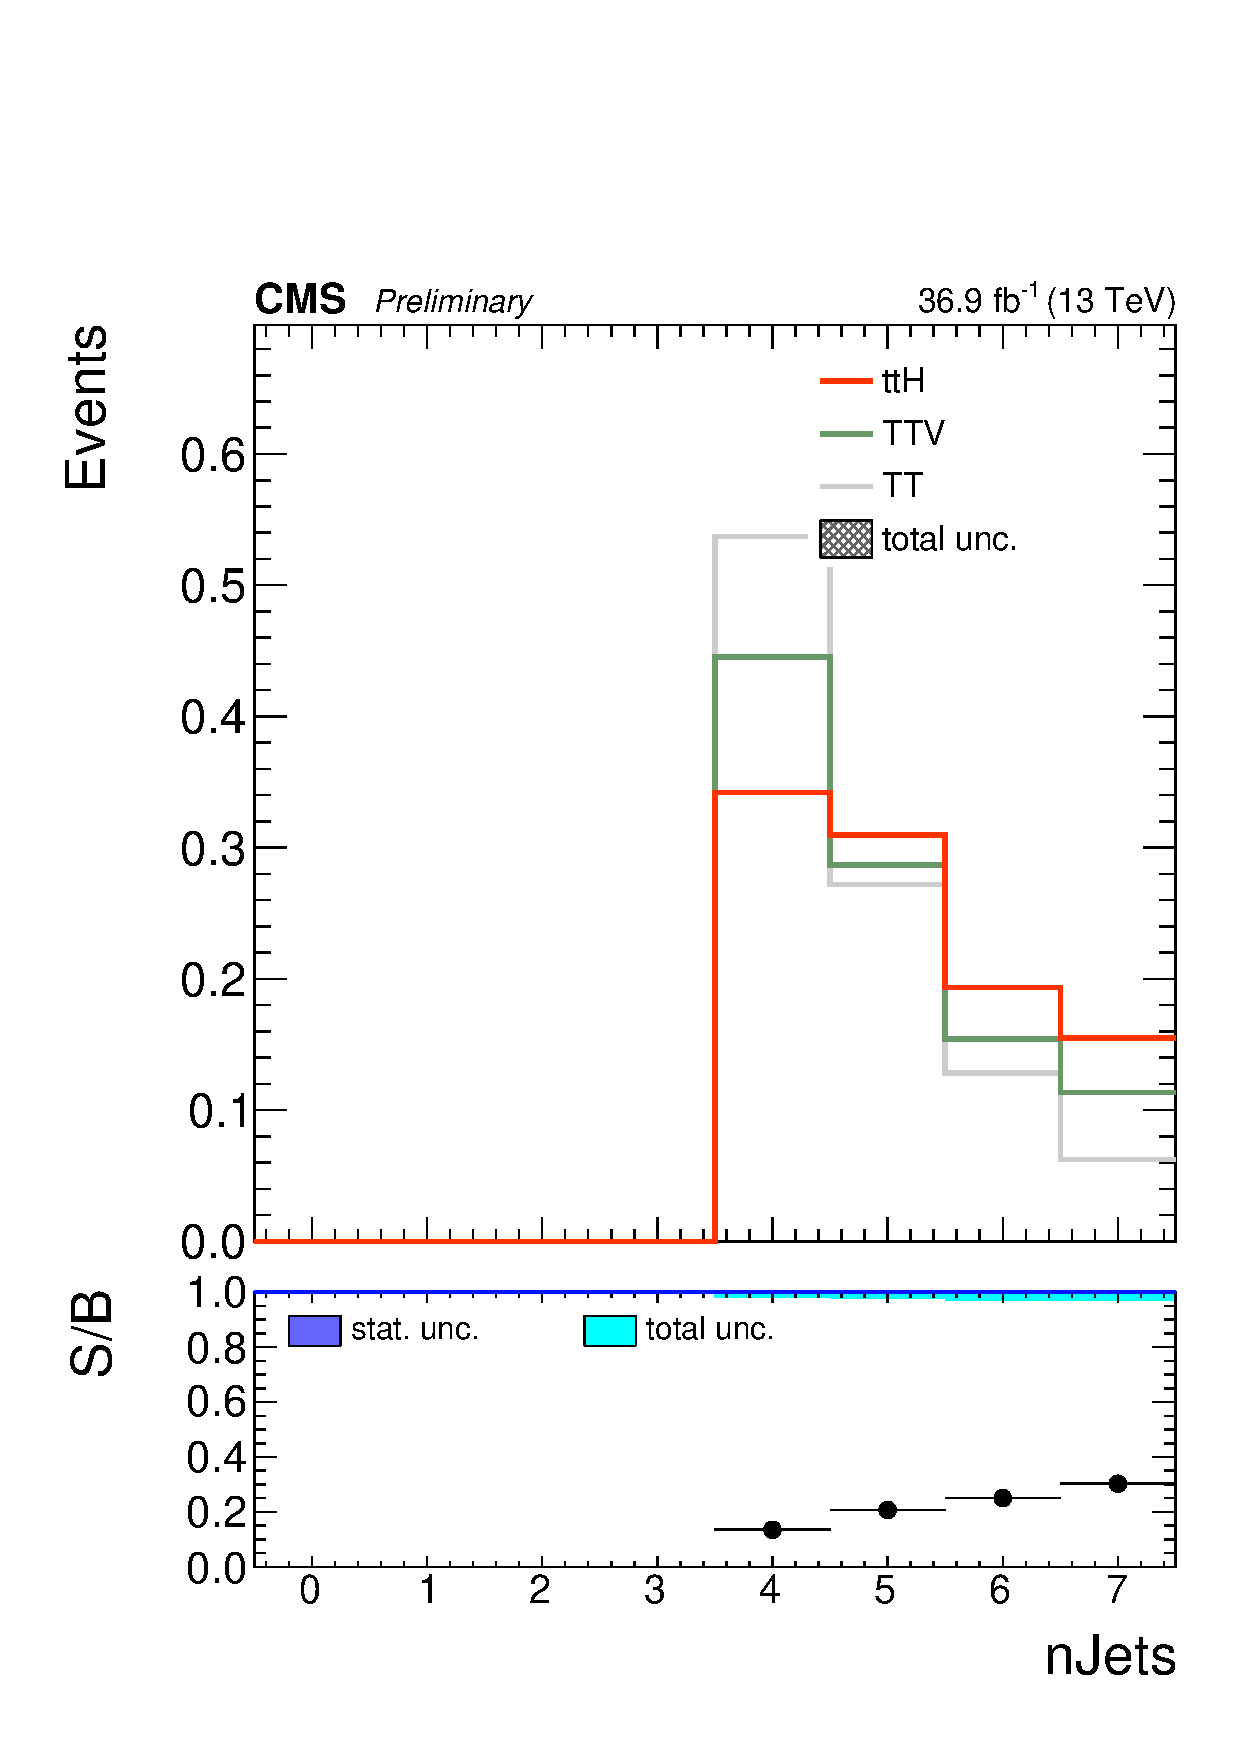
\includegraphics[width=0.32\textwidth]{plots_extraction/training/2lss/kinMVA_input_numJets.pdf}\\
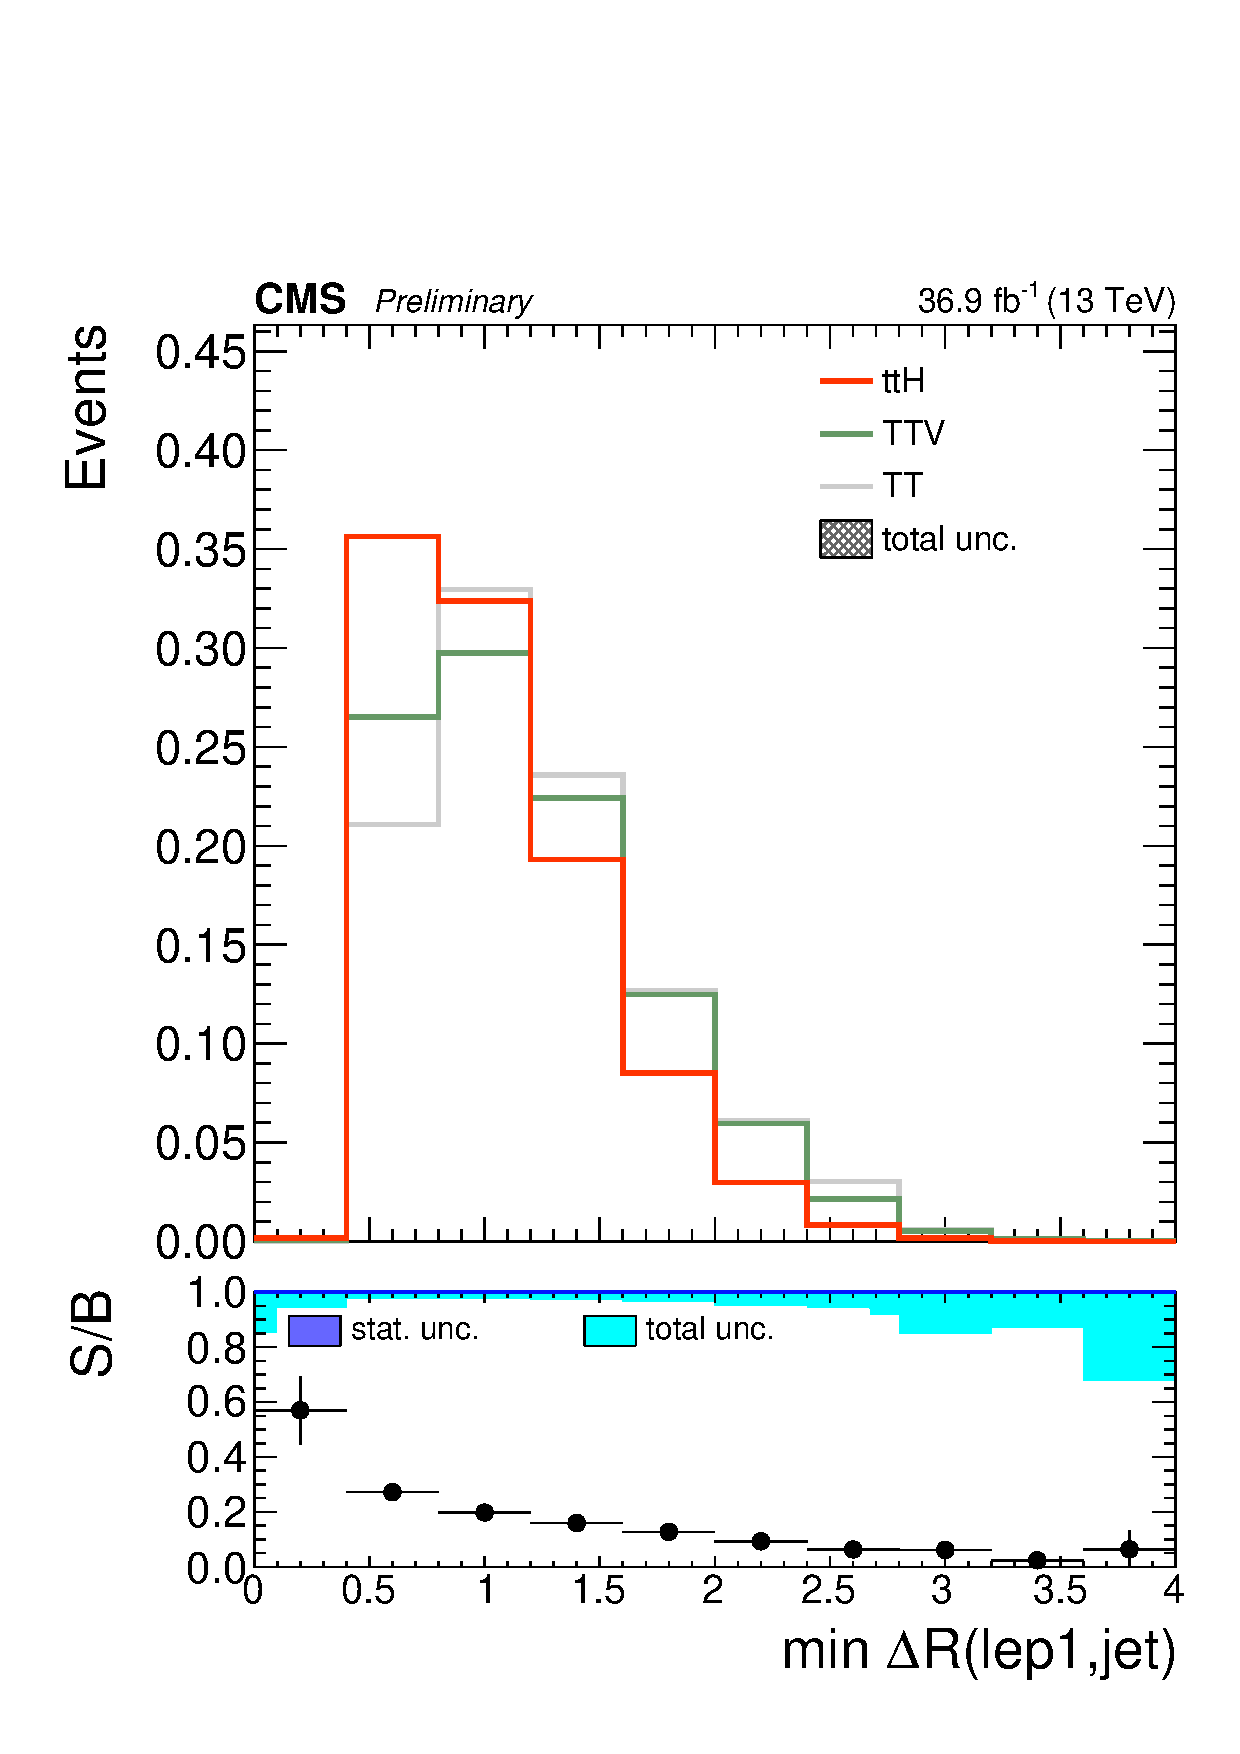
\includegraphics[width=0.32\textwidth]{plots_extraction/training/2lss/kinMVA_input_mindr_lep1_jet.pdf}
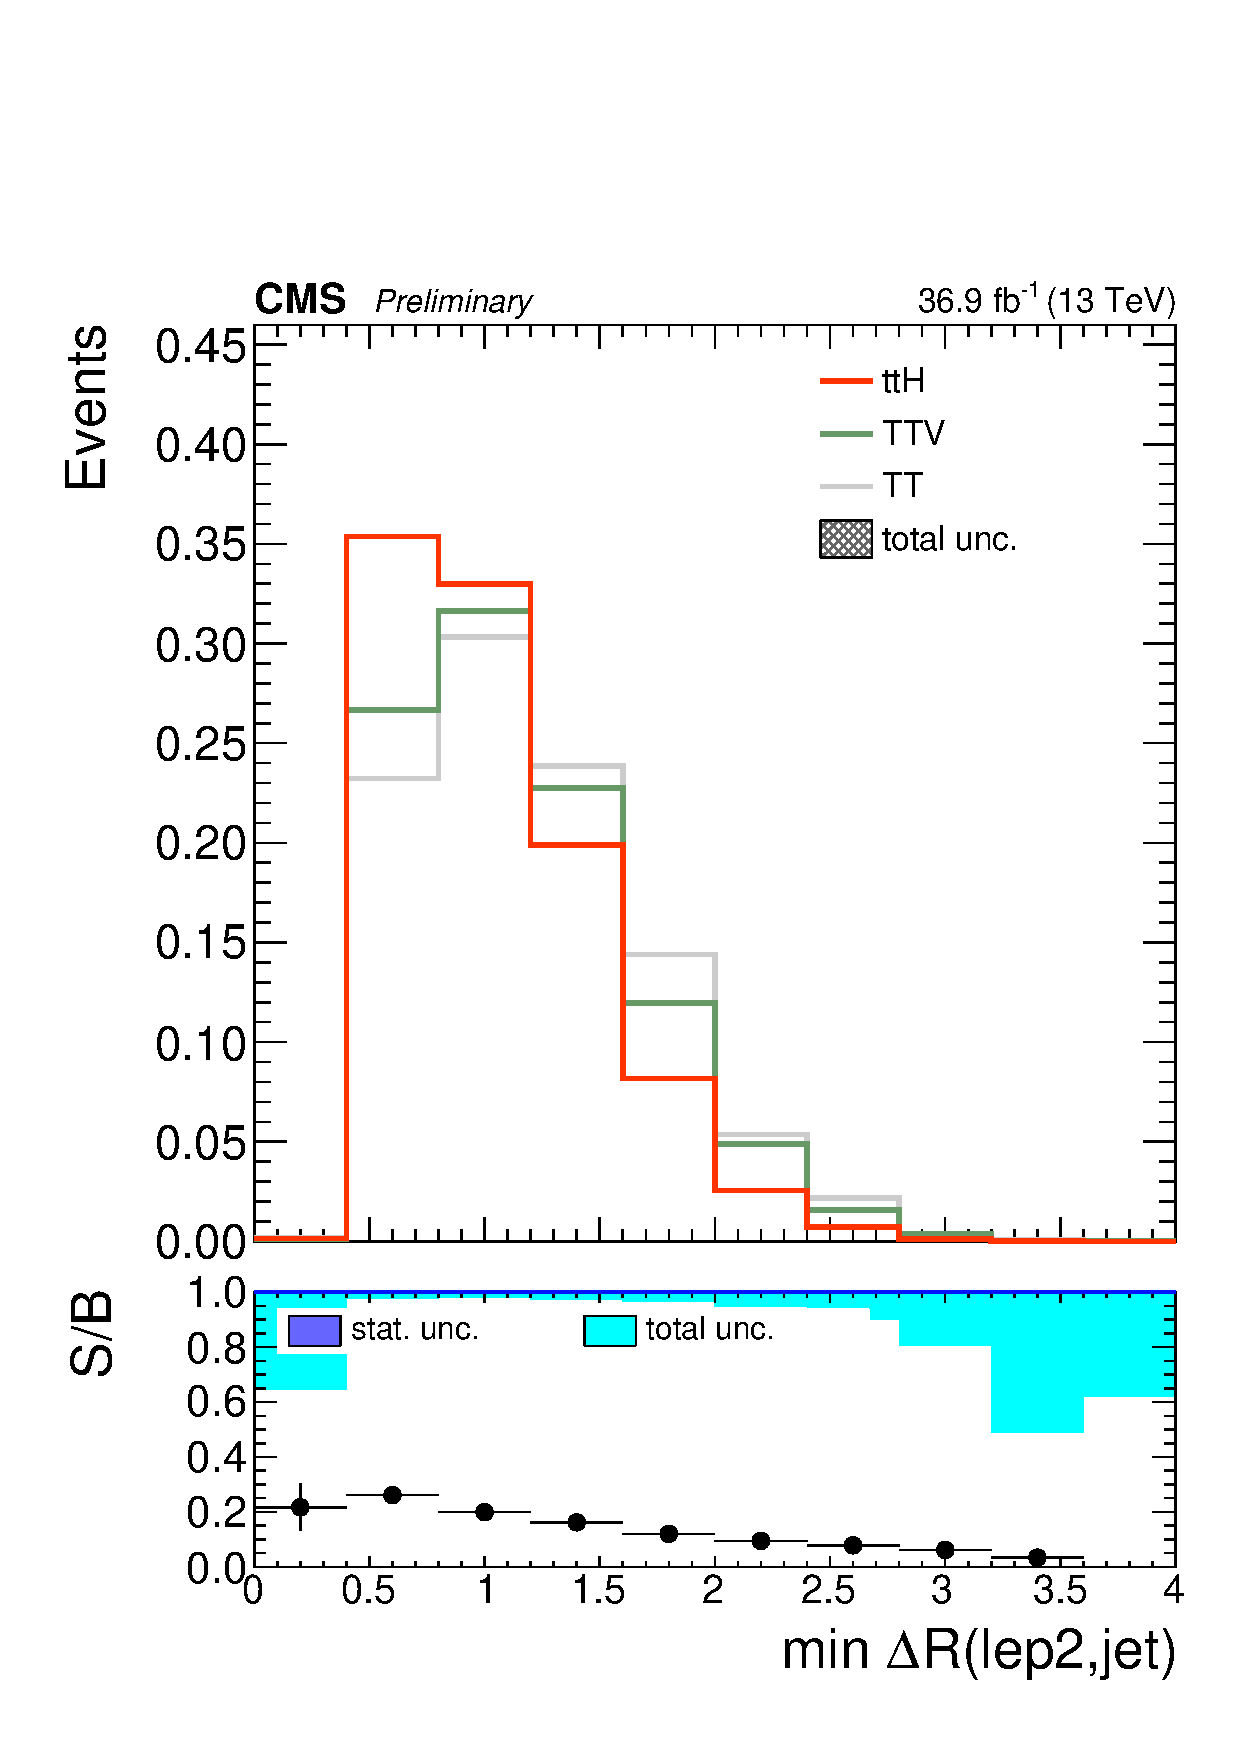
\includegraphics[width=0.32\textwidth]{plots_extraction/training/2lss/kinMVA_input_mindr_lep2_jet.pdf}
%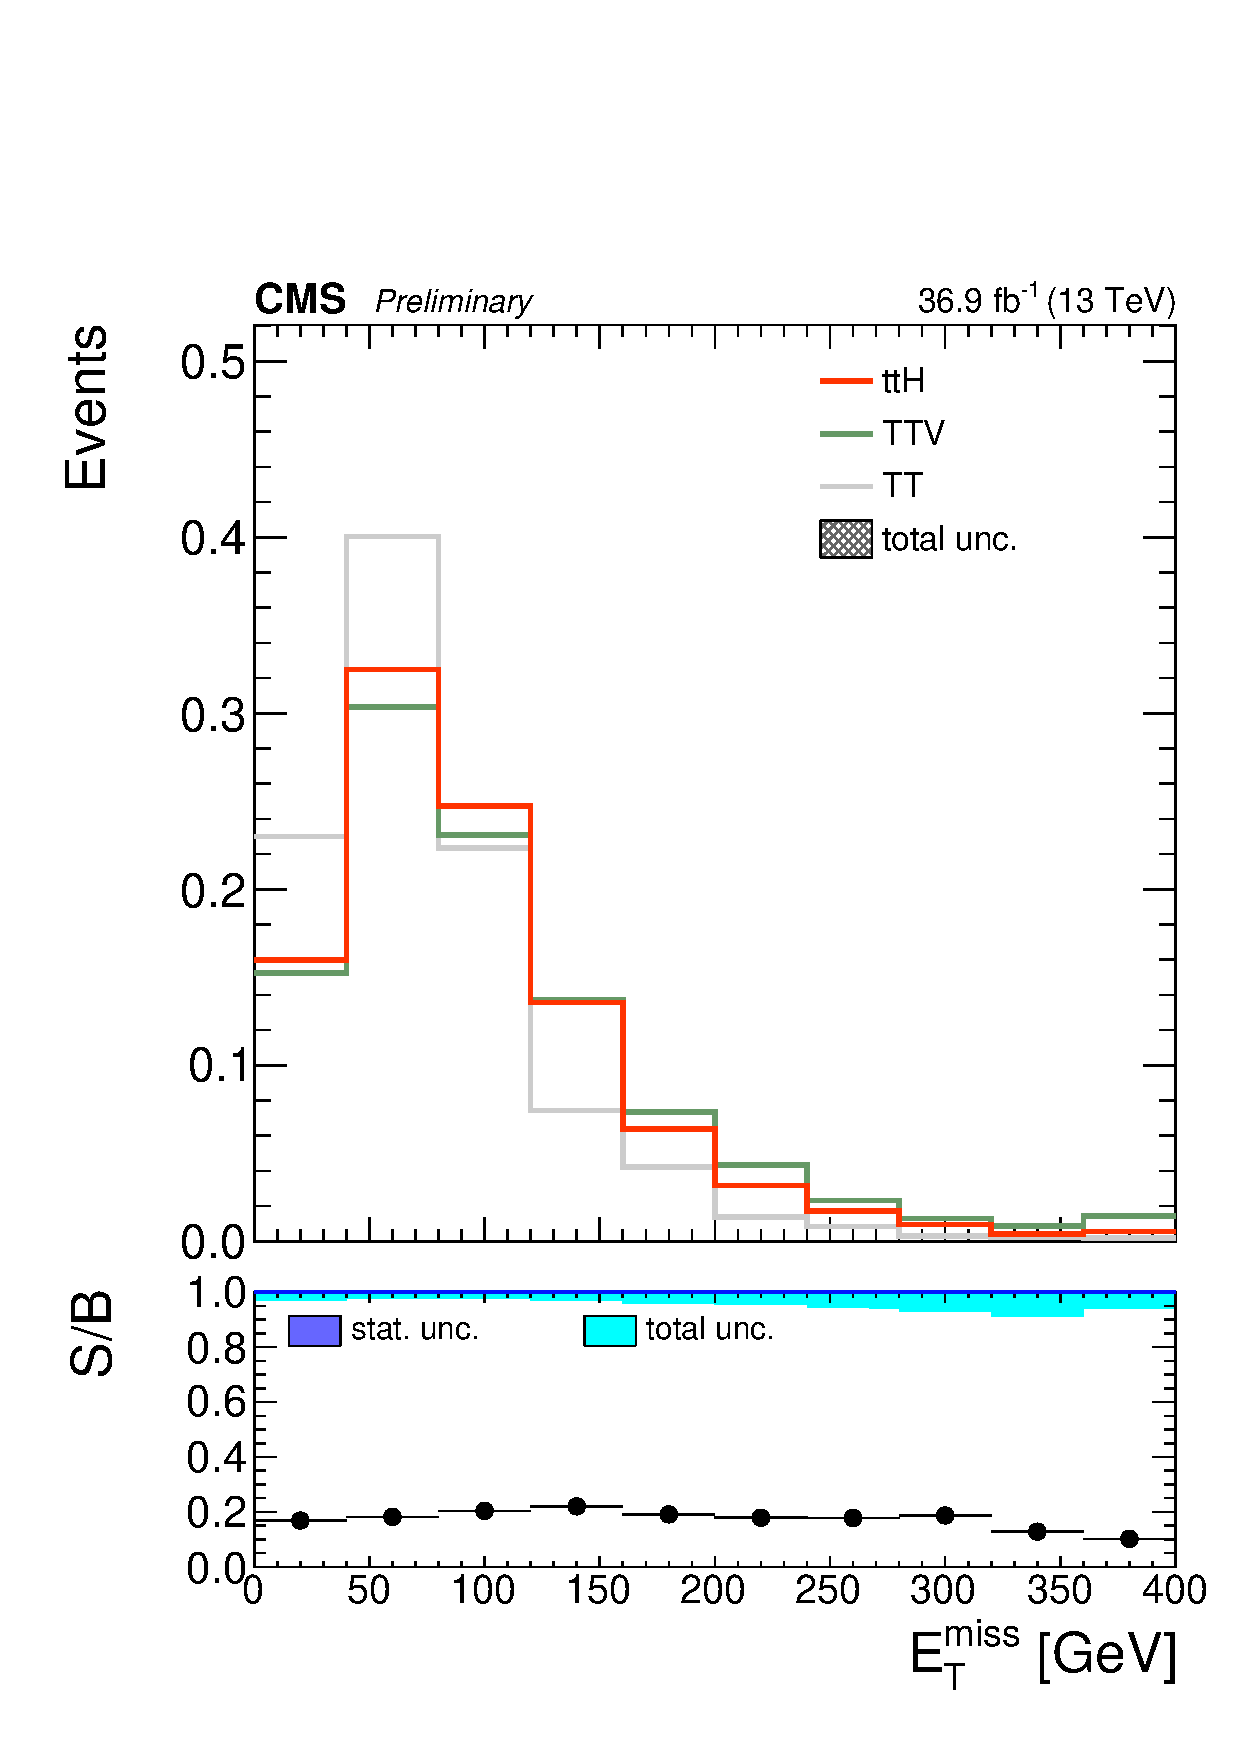
\includegraphics[width=0.32\textwidth]{plots_extraction/training/2lss/kinMVA_input_met.pdf}
%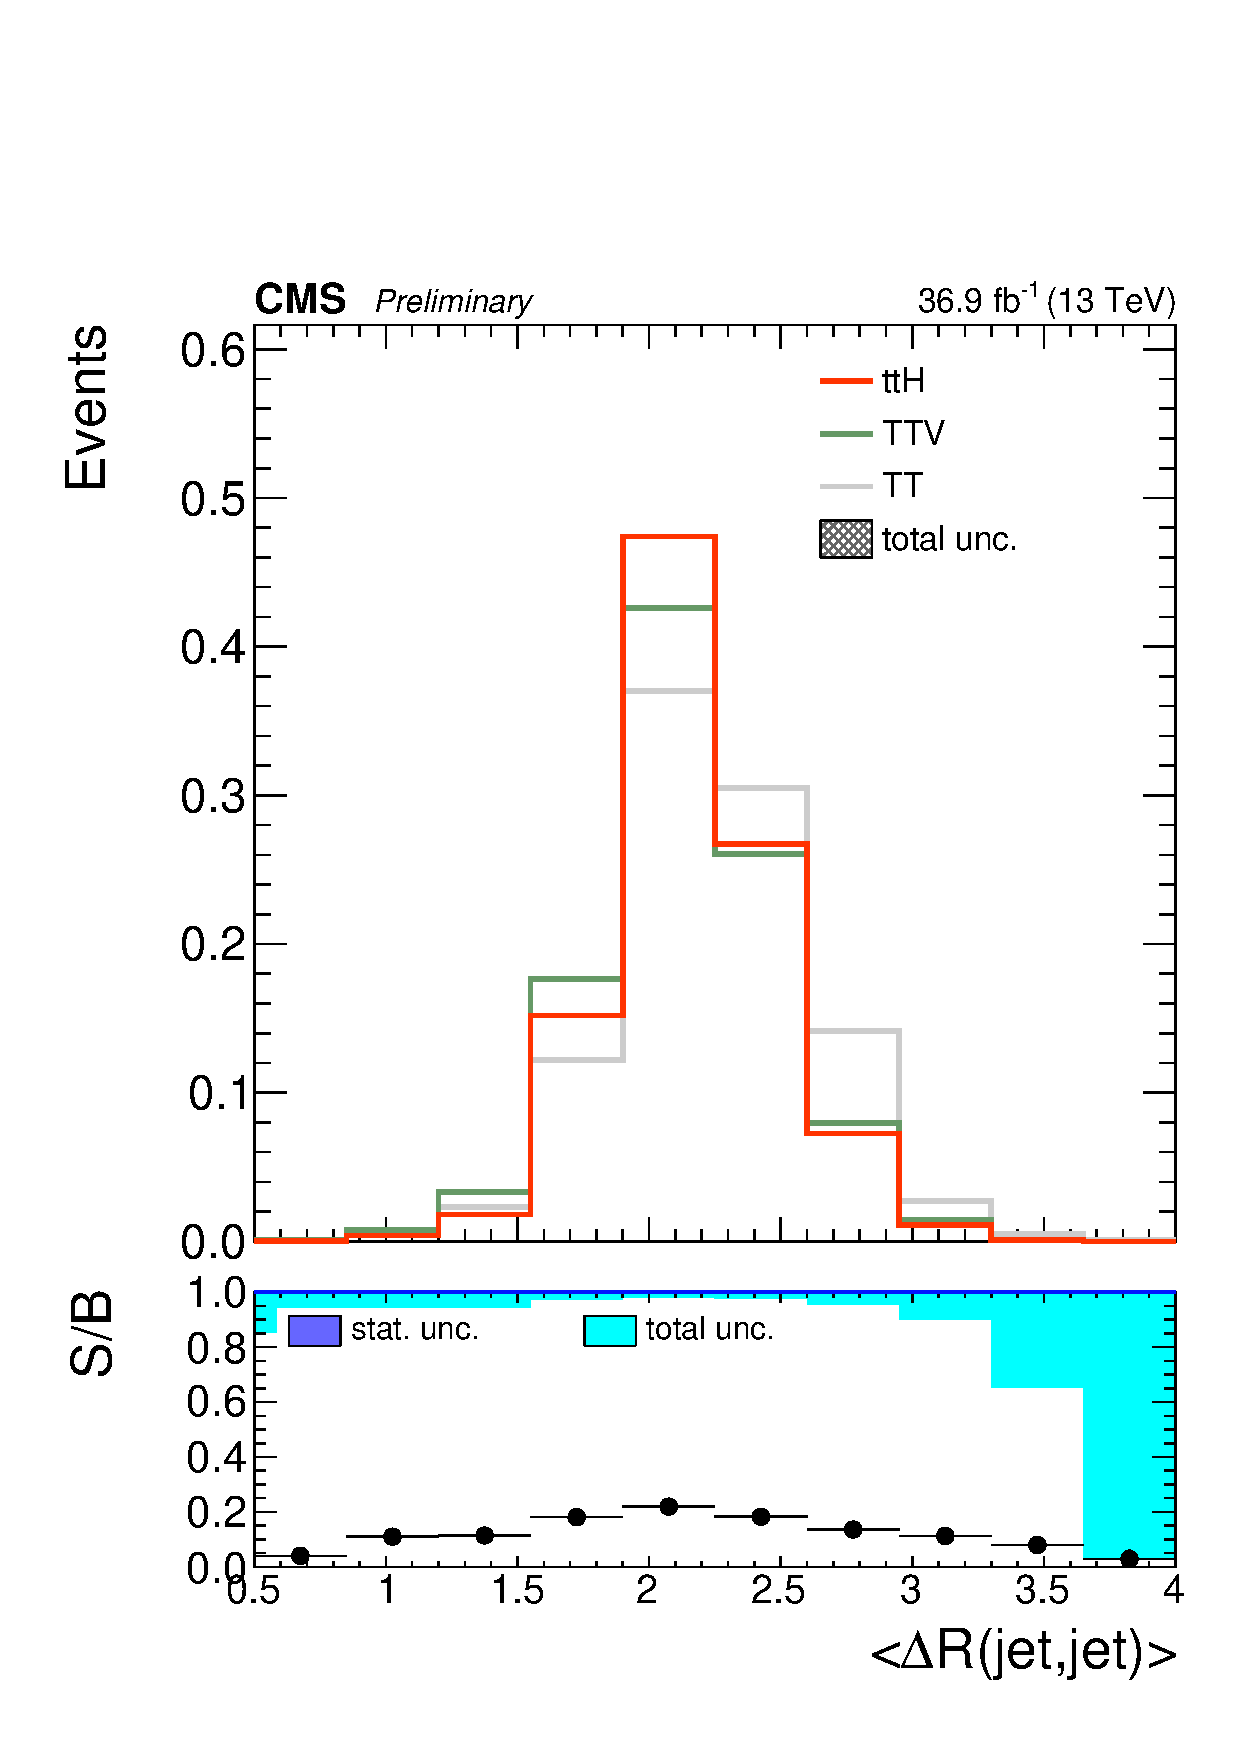
\includegraphics[width=0.32\textwidth]{plots_extraction/training/2lss/kinMVA_input_avg_dr_jet.pdf}
        \caption{The separation power of the variables used for BDT trainings, in the two same sign leptons channel.}
        \label{fig:2lss_training_1}
\end{figure}

\begin{figure}[htb]
        \centering
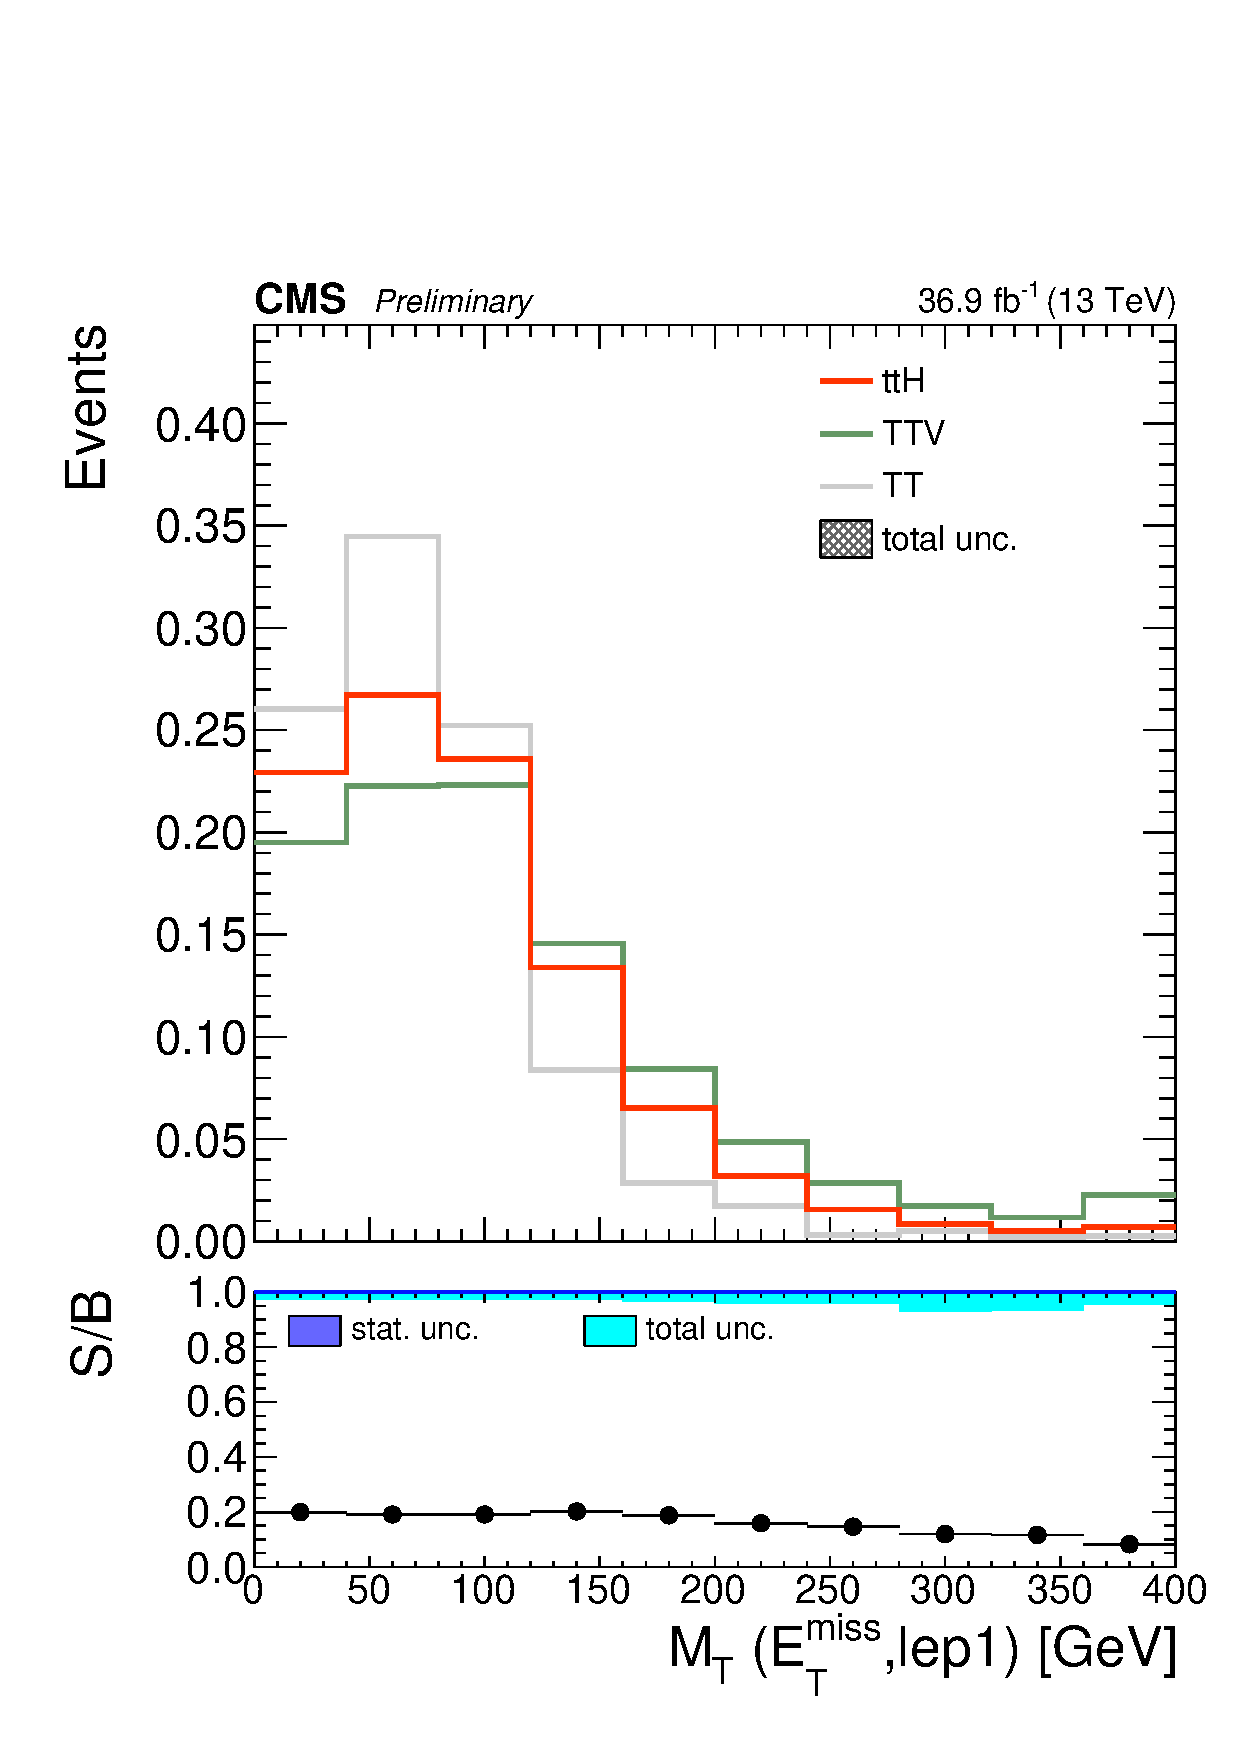
\includegraphics[width=0.32\textwidth]{plots_extraction/training/2lss/kinMVA_input_MT_met_lep1.pdf}
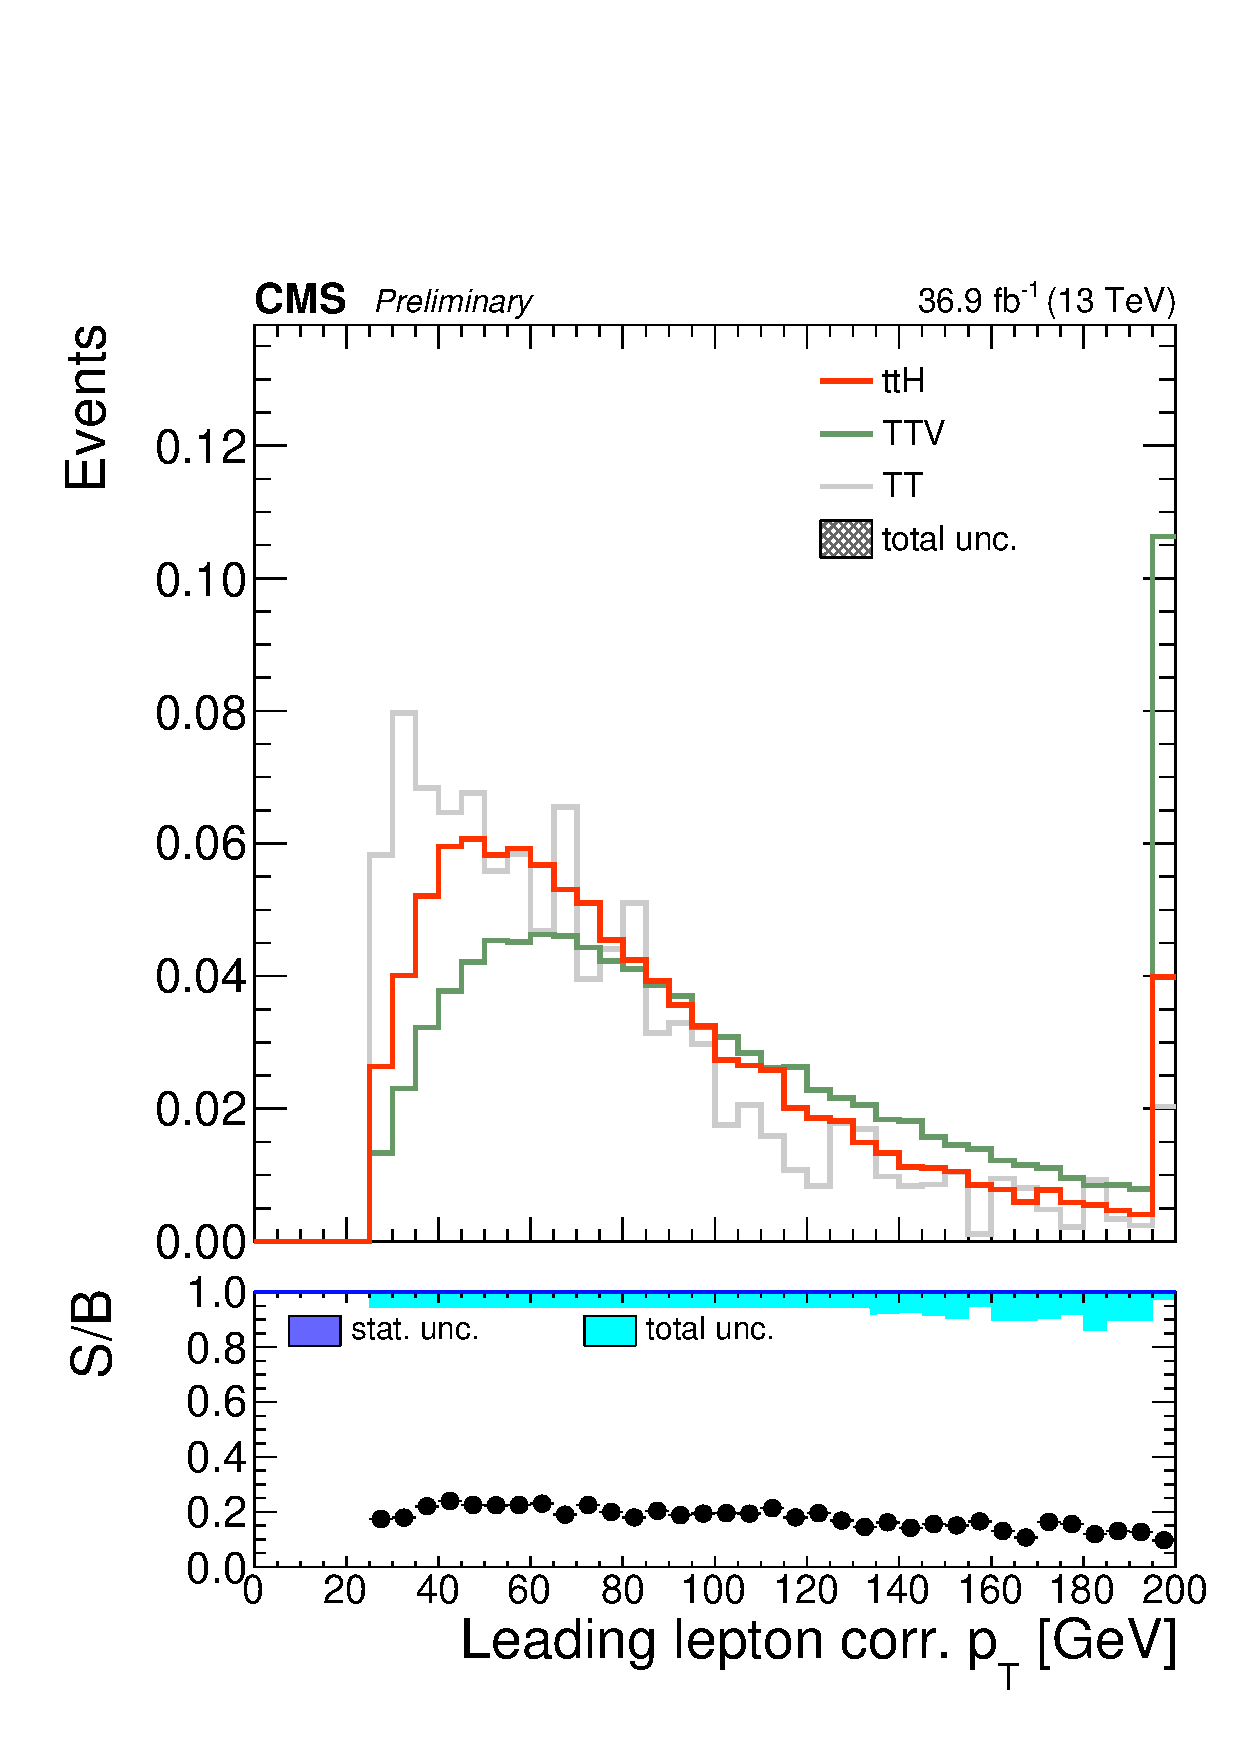
\includegraphics[width=0.32\textwidth]{plots_extraction/training/2lss/kinMVA_input_LepGood0_conePt.pdf}\\
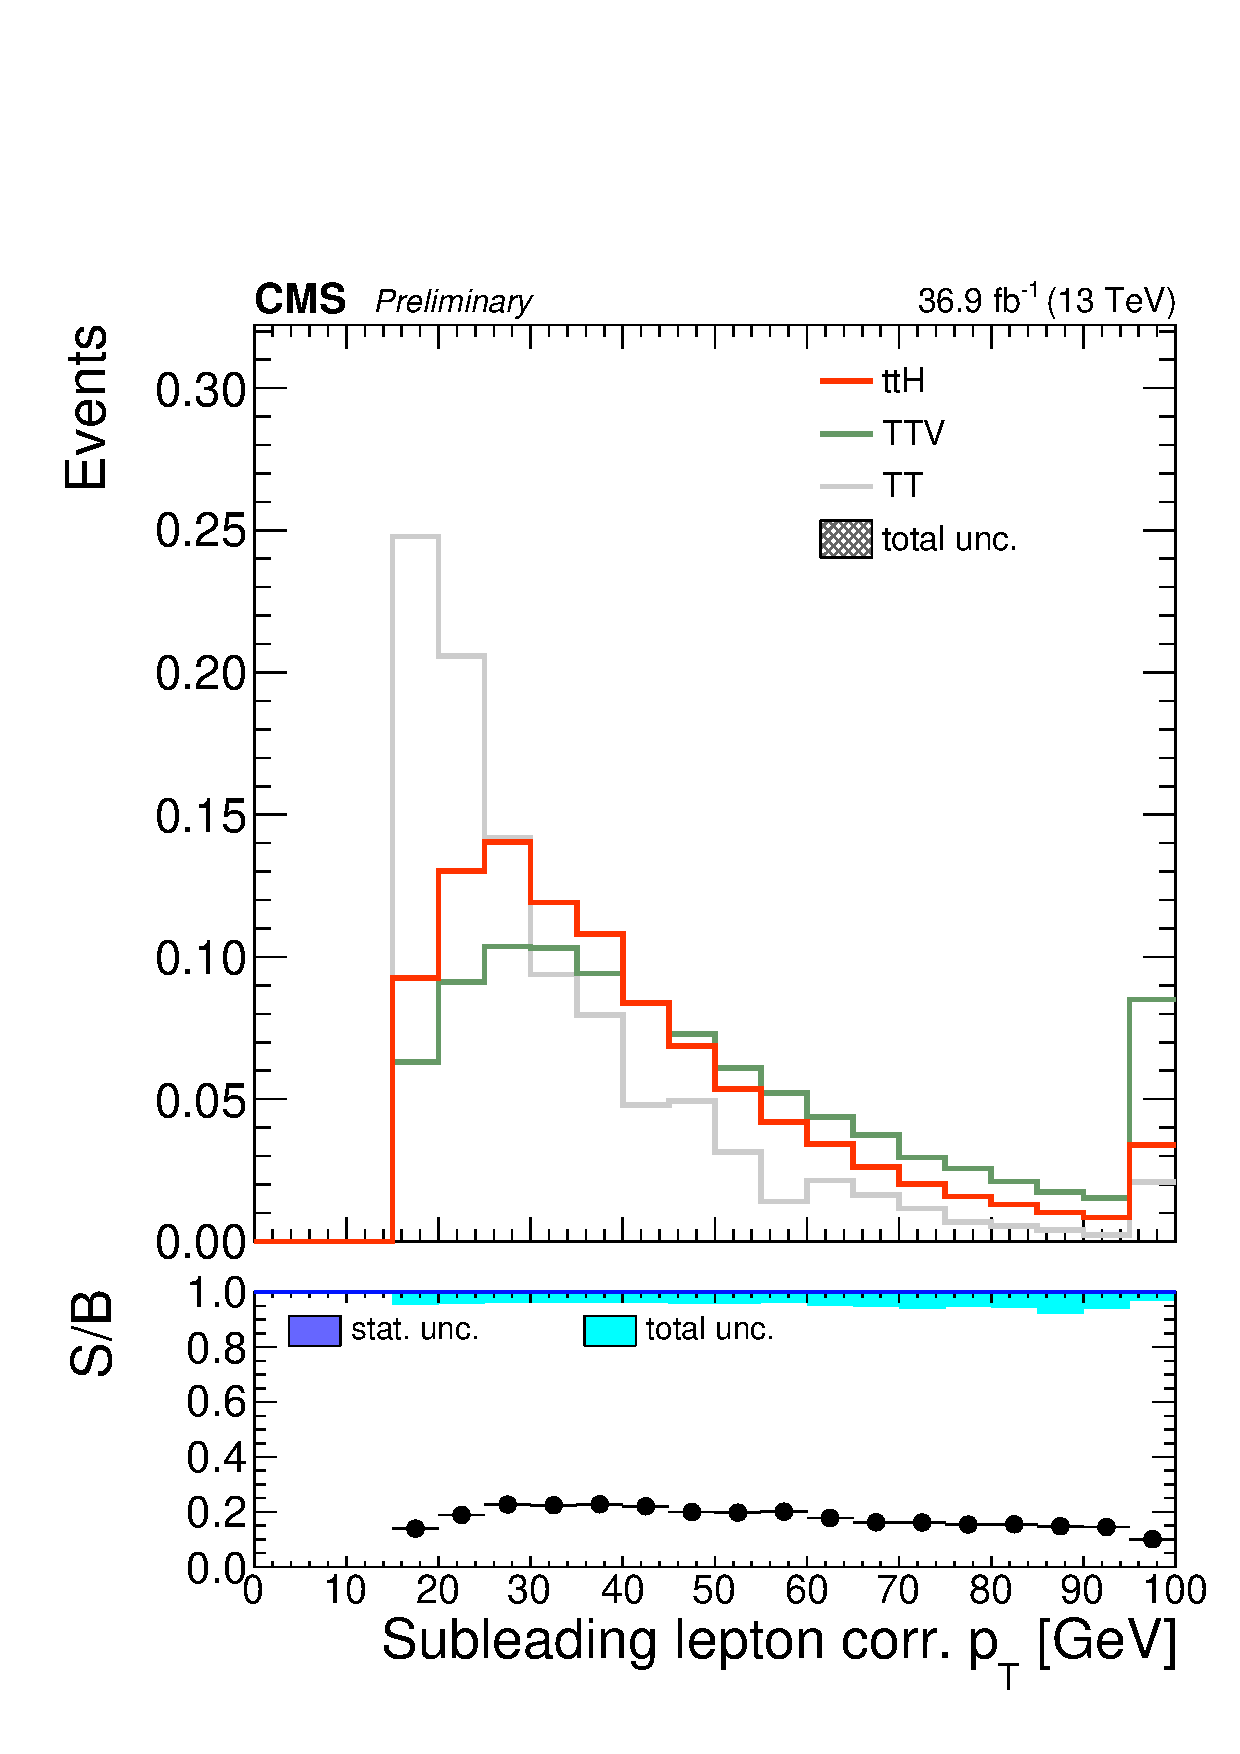
\includegraphics[width=0.32\textwidth]{plots_extraction/training/2lss/kinMVA_input_LepGood1_conePt.pdf}
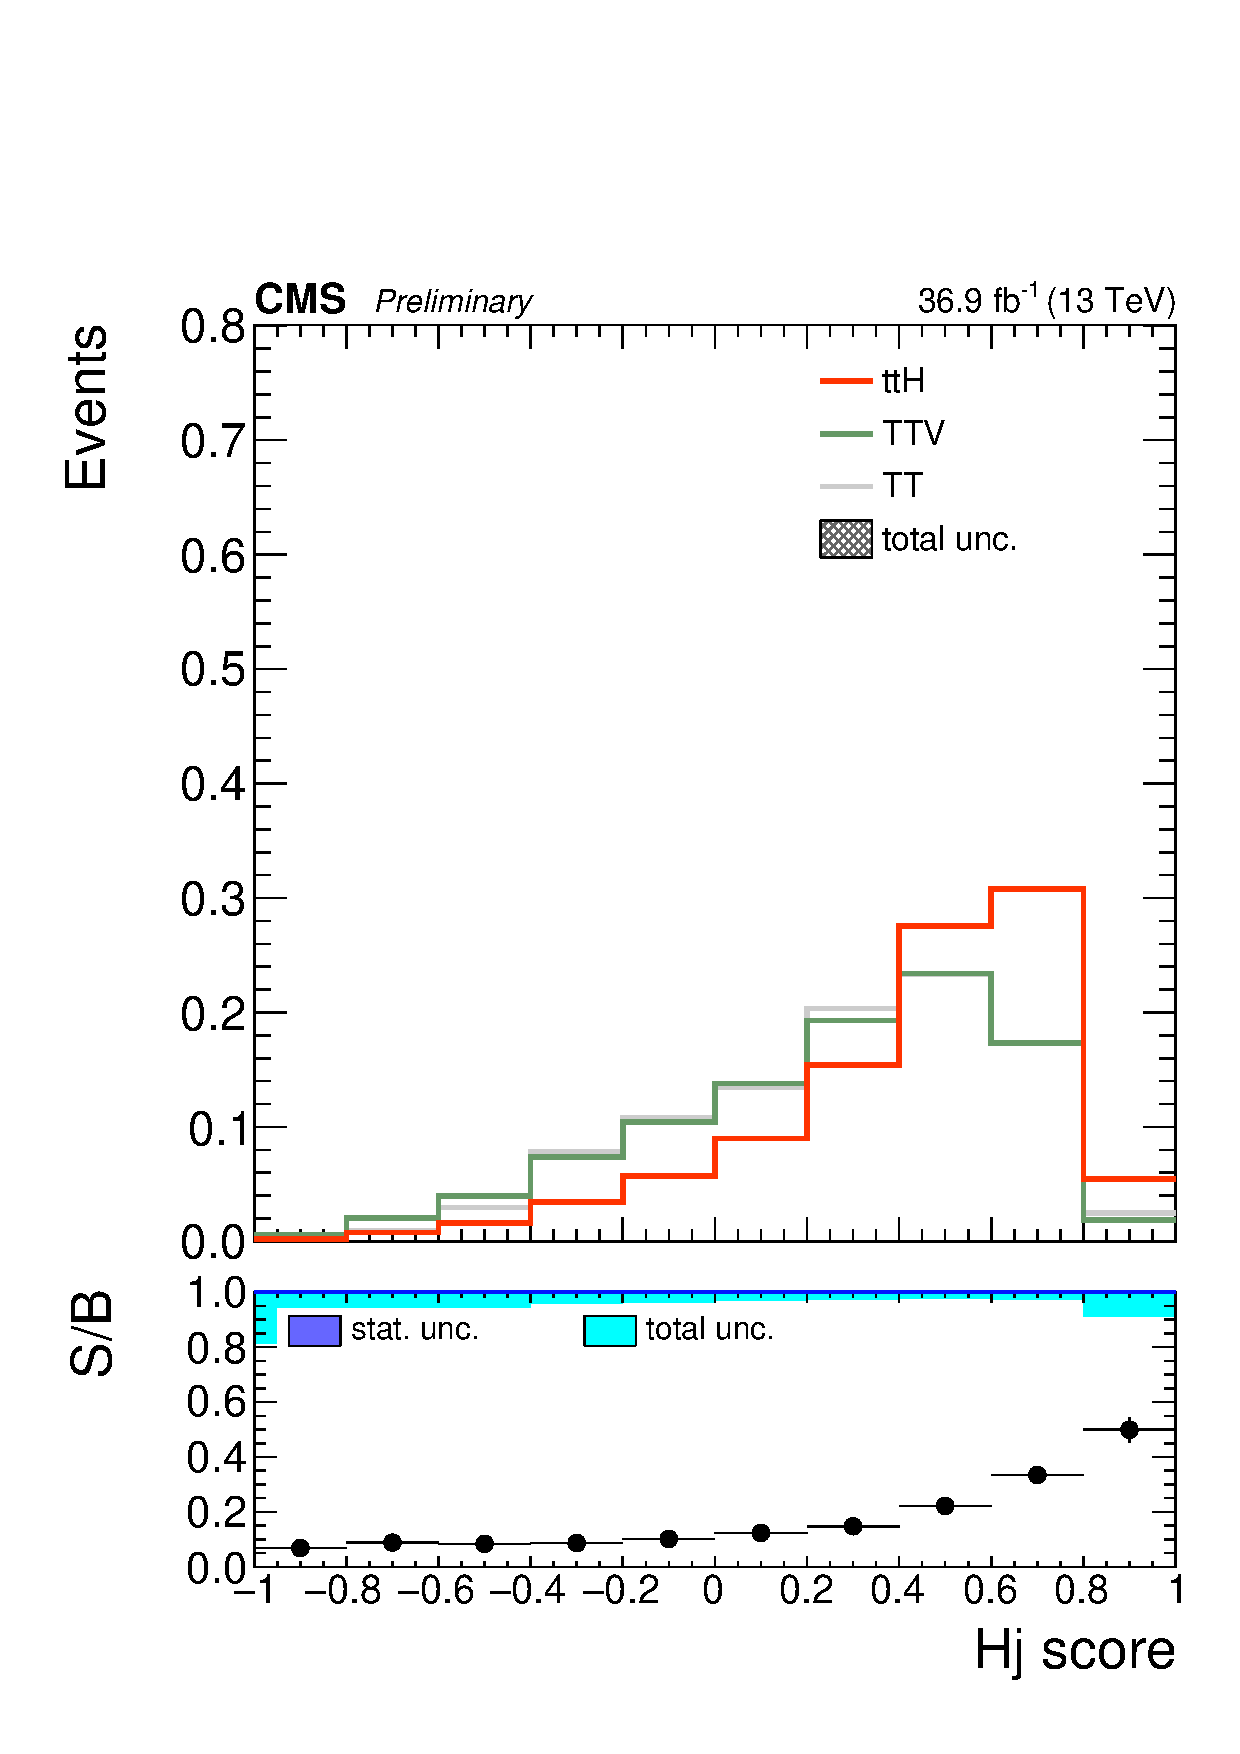
\includegraphics[width=0.32\textwidth]{plots_extraction/training/2lss/kinMVA_input_BDTv8_eventReco_Hj_score.pdf}
%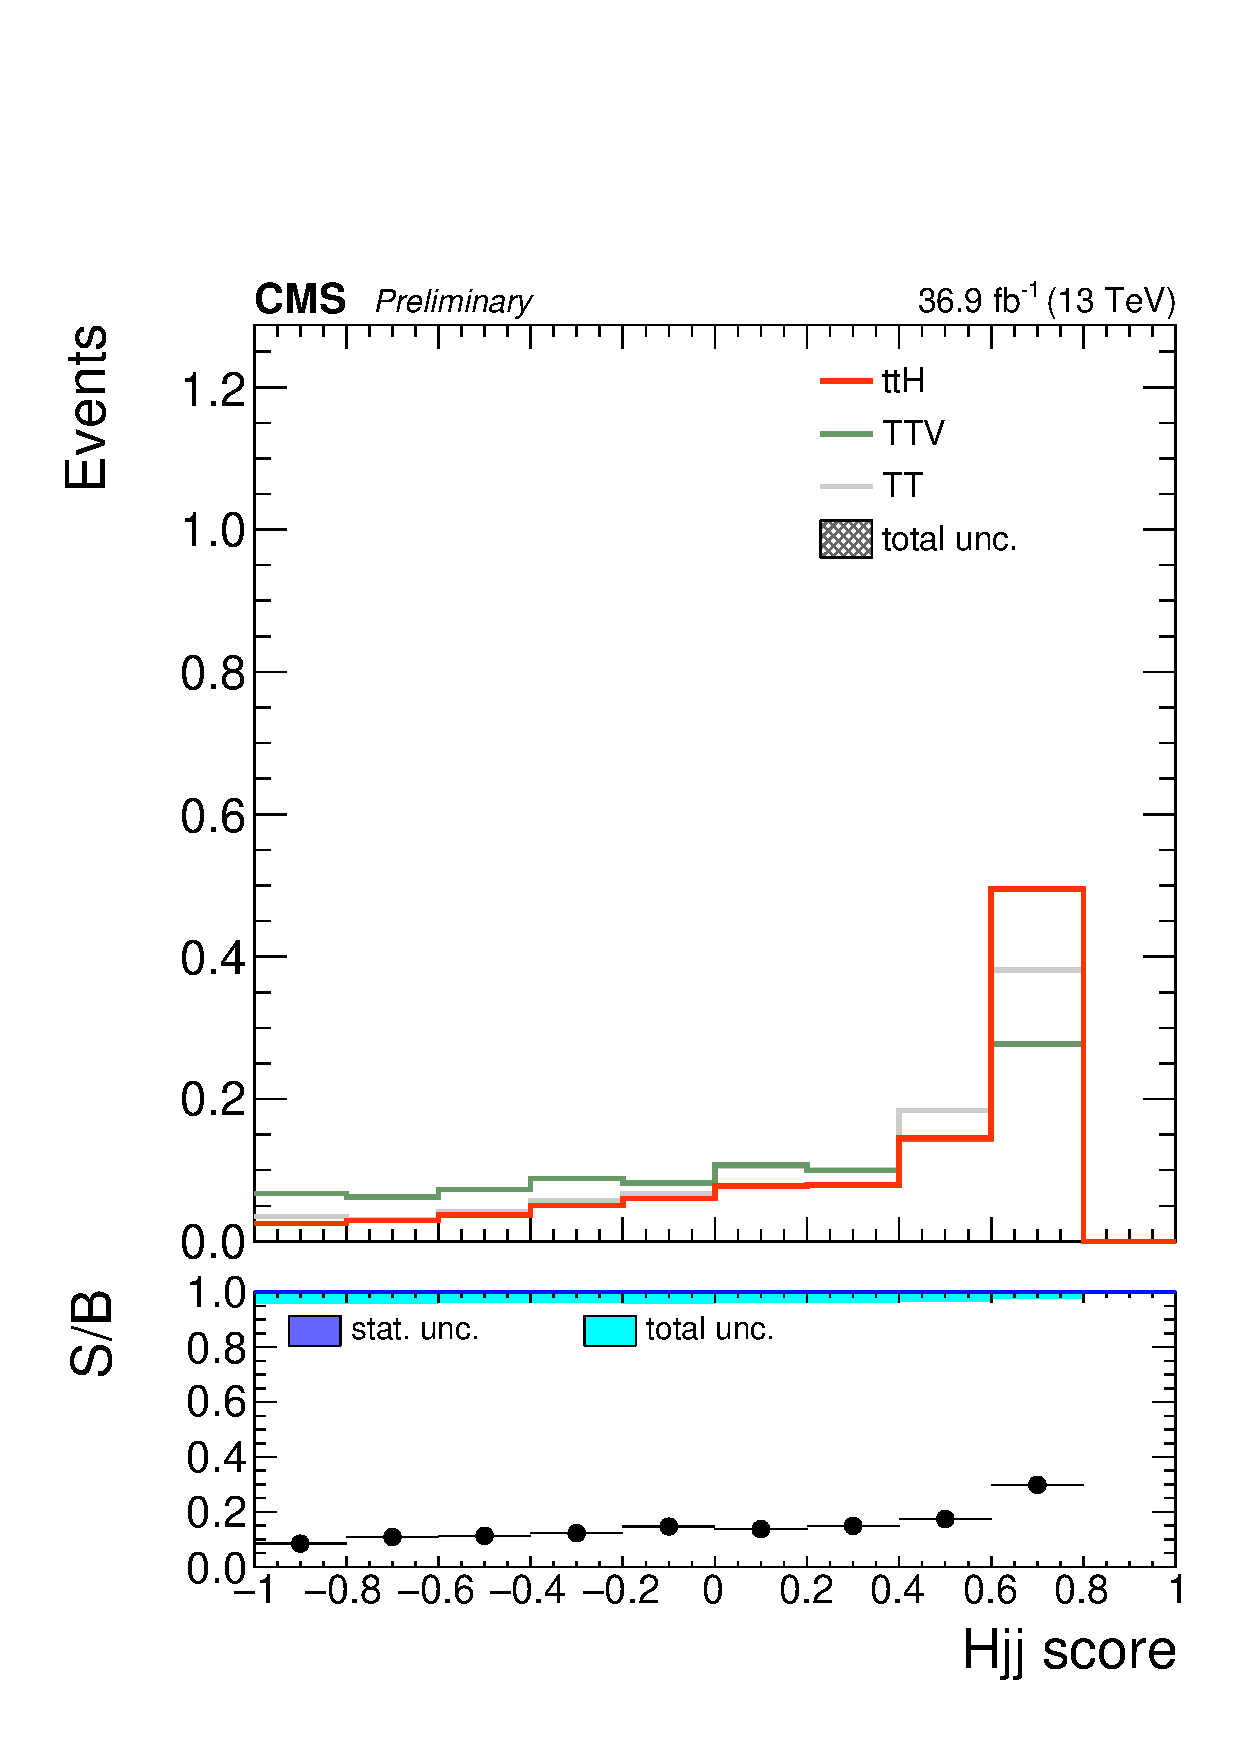
\includegraphics[width=0.32\textwidth]{plots_extraction/training/2lss/kinMVA_input_BDTv8_eventReco_Hjj_score.pdf}
        \caption{The separation power of the variables used for BDT trainings, in the two same sign leptons channel.}
        \label{fig:2lss_training_2}
\end{figure}

\begin{figure}[htb]
%\captionsetup[subfigure]{labelformat=empty}
	\centering
%\begin{subfigure}
	%\centering
\includegraphics[width=0.35\textwidth]{plots_extraction/training/2lss/kinMVA_2lss_ttbar_withBDTv8.pdf}%kinMVA_2lss_ttbar.pdf}
\includegraphics[width=0.35\textwidth]{plots_extraction/training/2lss/kinMVA_2lss_ttV_withHj.pdf}%kinMVA_2lss_ttV.pdf}
	\caption{The separation power of the BDT output against the ttbar (left) and ttV (right) background, in the two same sign leptons channel.}
	\label{fig:2l_mvaTraining}
\end{figure}
%\end{subfigure}
%\bigskip
%\bigskip

%\begin{figure}[htb]
%	\centering
%%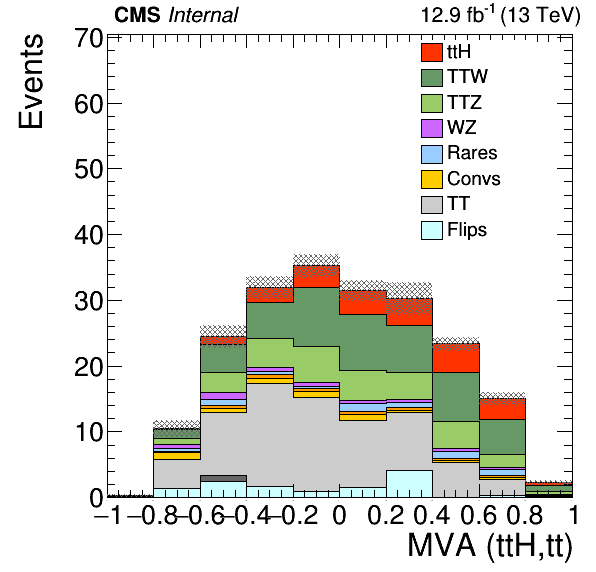
\includegraphics[width=0.35\textwidth]{plots_extraction/selection/2lss_SR/kinMVA_2lss_ttbar}
%%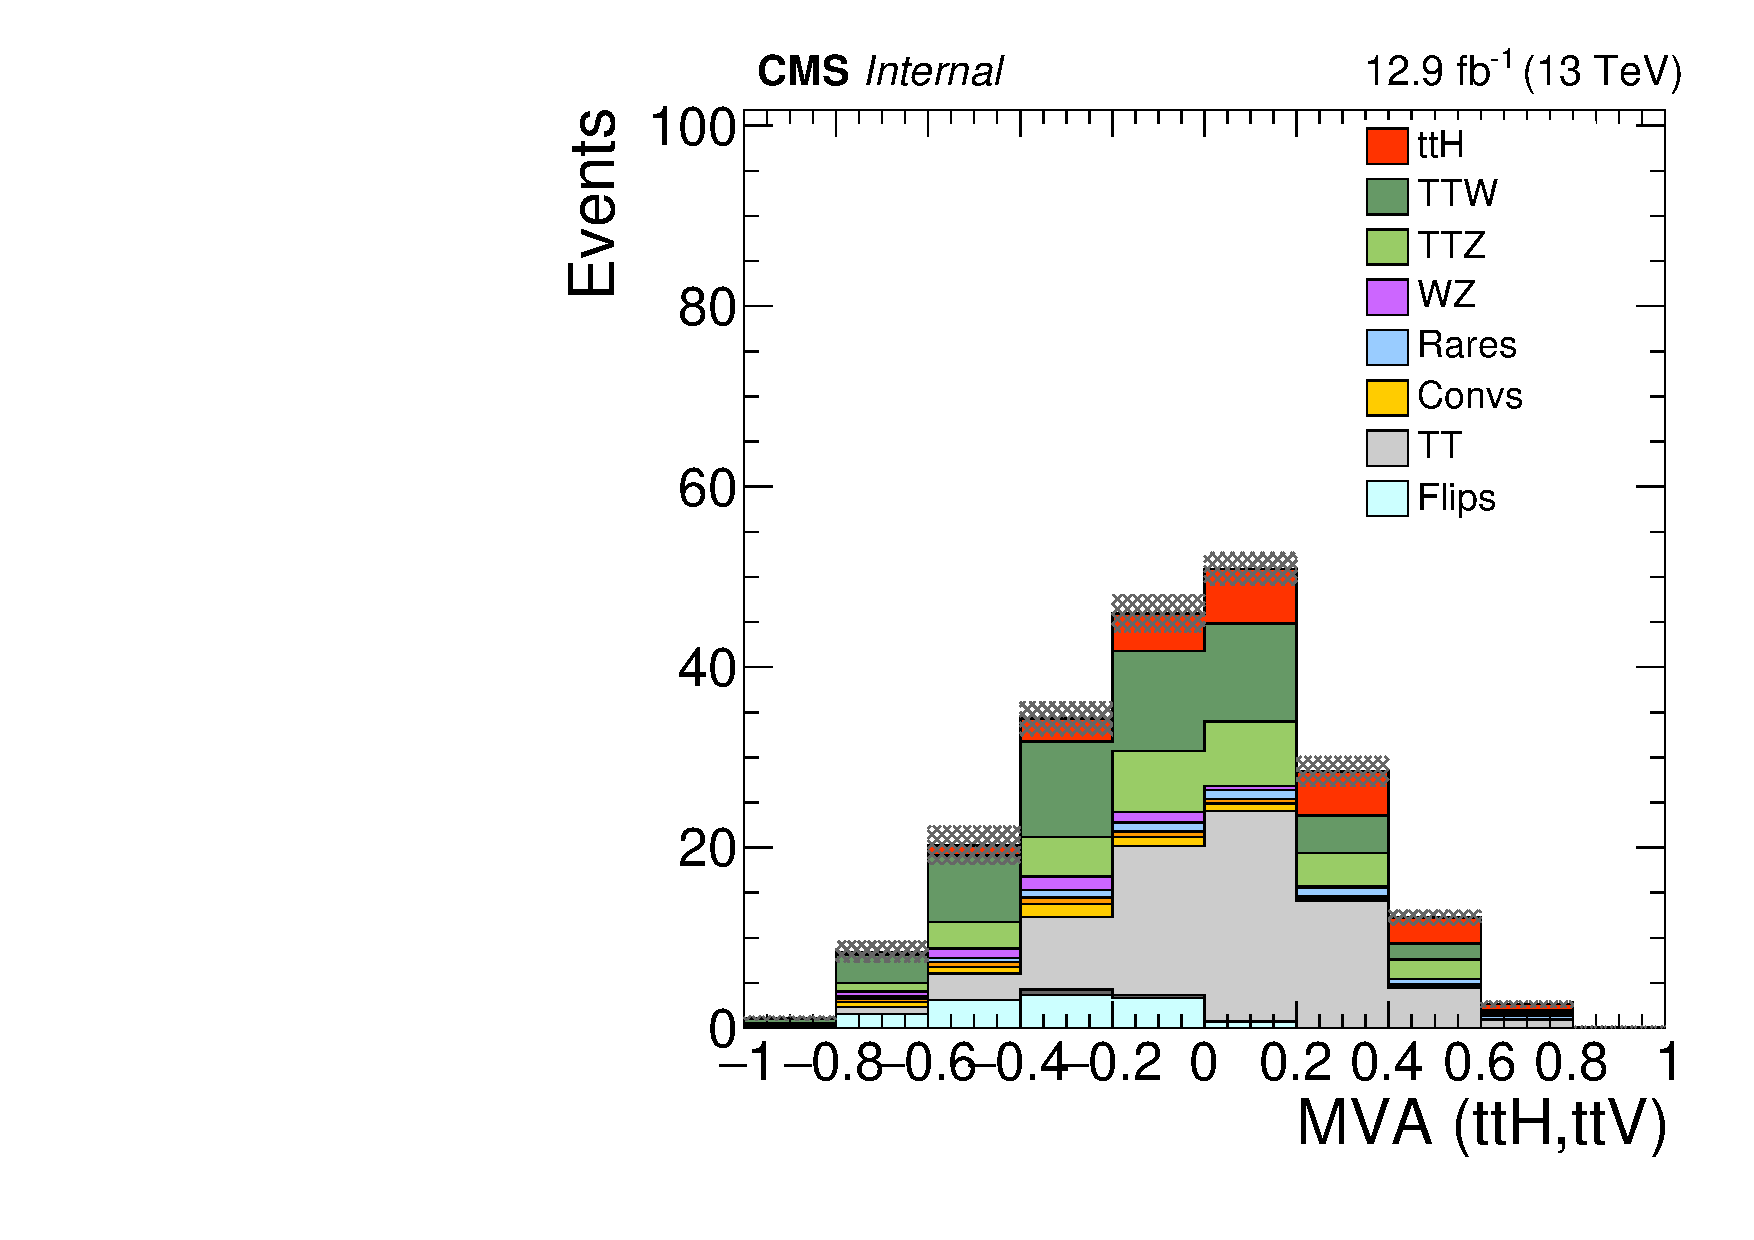
\includegraphics[width=0.35\textwidth]{plots_extraction/selection/2lss_SR/kinMVA_2lss_ttV}\\
%\includegraphics[width=0.35\textwidth]{plots_extraction/selection_data/2lss_SR/kinMVA_2lss_ttbar_withBDTv8.pdf}
%\includegraphics[width=0.35\textwidth]{plots_extraction/selection_data/2lss_SR/kinMVA_2lss_ttV_withHj.pdf}
%	\caption{Distribution of the discriminator against the ttbar (left) and ttV (right) backgrounds, in the two same sign leptons channel, with reducible background prediction from MC (top) and from data (bottom).}
%	\label{fig:2l_mvaOutput}
%\end{figure}

\clearpage
\subsection{3l event BDT}\label{sec:3lss event BDT}
The three lepton category has the following variables for the training against the \ttbar\ background:
\begin{itemize}
\item maximum absolute pseudorapidity of the two leading leptons
\item multiplicity of hadronic jets
\item minimum distance between the leading lepton and closest jet
\item minimum distance of the trailing lepton and closest jet.
\item transverse mass of the leading lepton and missing transverse energy
%\item missing HT
%\item average distance of the two jets
\end{itemize}

For the training against the \ttV\ background, the input variables are:
\begin{itemize}
\item maximum absolute pseudorapidity of the two leading leptons
\item transverse mass of the leading lepton and missing transverse energy
\item multiplicity of hadronic jets
\item minimum distance between the leading lepton and closest jet
\item minimum distance of the trailing lepton and closest jet
\item leading lepton transverse momentum and the third lepton transverse momentum.
\end{itemize}

Furthermore, the performance of the Matrix Element Method (MEM, as described in Appendix.~\ref{sec:mem}, on page~\pageref{sec:mem}) in the three lepton category warrants its inclusion as input to the training against the \ttV\ process. For ICHEP2016, the MEM was included using the log of weights for the \ttH, \ttW\ and \ttZ\ hypotheses.
For this iteration of the analysis, it was found that given the \ttV\ BDT parameters used, it is more efficient to include solely the likelihood of background vs signal + backgrounds (one variable instead of three). This improves the performance by a few percent.

In addition, it was found that the \ttbar\ BDT could also be improved by including the MEM among the input variables, using the MEM weights of \ttH, \ttbar, and the weights obtained from kinematic reconstruction of fully and semi leptonic ttH hypothesis are included. It improves the performance of the \ttbar\ BDT by about 5\%. \textit{In the current version of the analysis, this is not yet implemented because of CPU time constraints (MEM not yet run on the \ttbar\ sample).}

Because the currently available Monte-Carlo statistics prevent us from training with the full event selection, a relaxed selection has been
applied instead for training. This relaxed selection requires at least three preselected leptons where neither lepton pair has an invariant mass within
10 GeV of the mass of the Z boson, the leading, trailing and sub-trailing lepton transverse momentum larger than 25, 15 and 15 GeV,
respectively, the MET LD requirement applied and at least two loose selected b-jets in the event.
In Figures~\ref{fig:3l_training_1} and~\ref{fig:3l_training_2} a comparison of the simulated signal (ttH) and background (\ttbar\ or \ttV) processes for each of the input variables
to the BDT discriminator is presented. Further details on the BDT training are available in Appendix~\ref{app:BDTtraining}.

\begin{figure}[htb]
        \centering
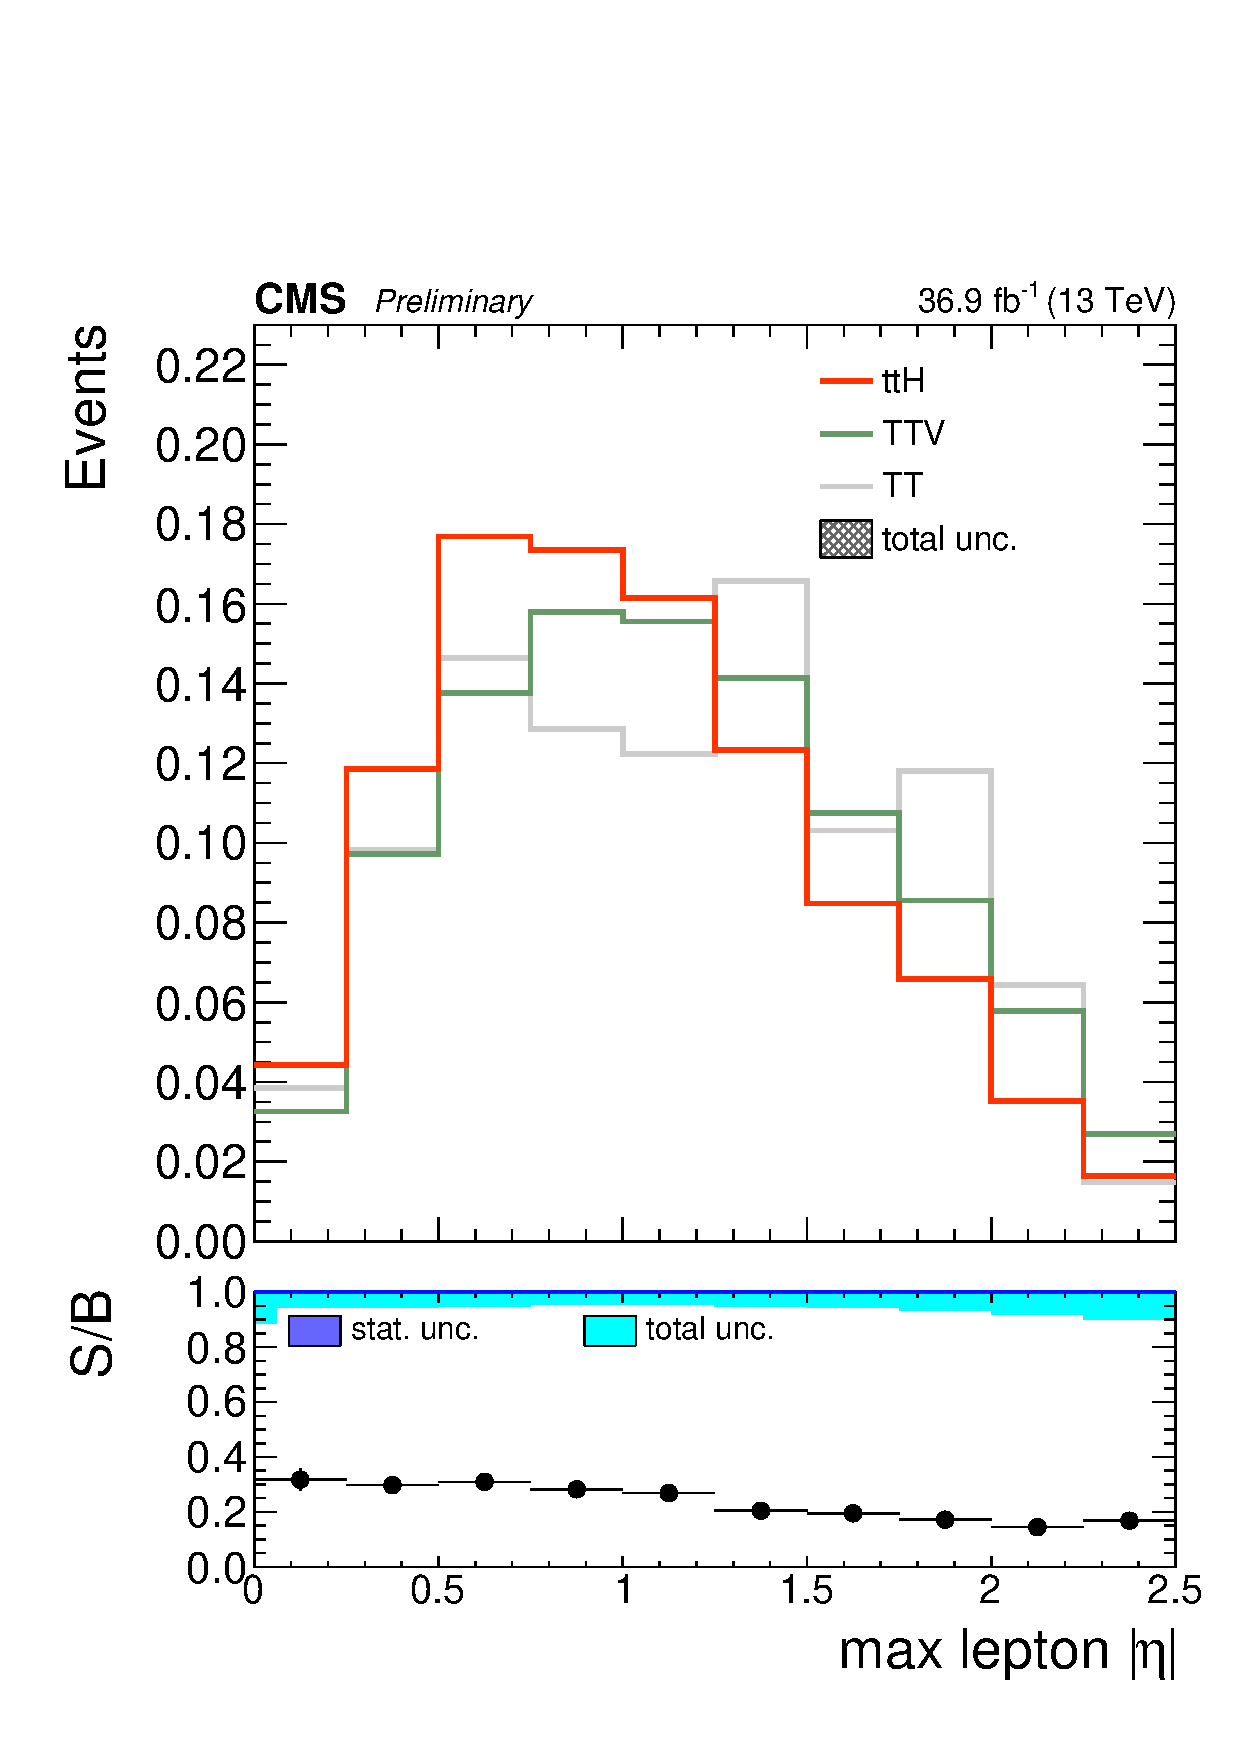
\includegraphics[width=0.32\textwidth]{plots_extraction/training/3l/kinMVA_input_max_Lep_eta.pdf}
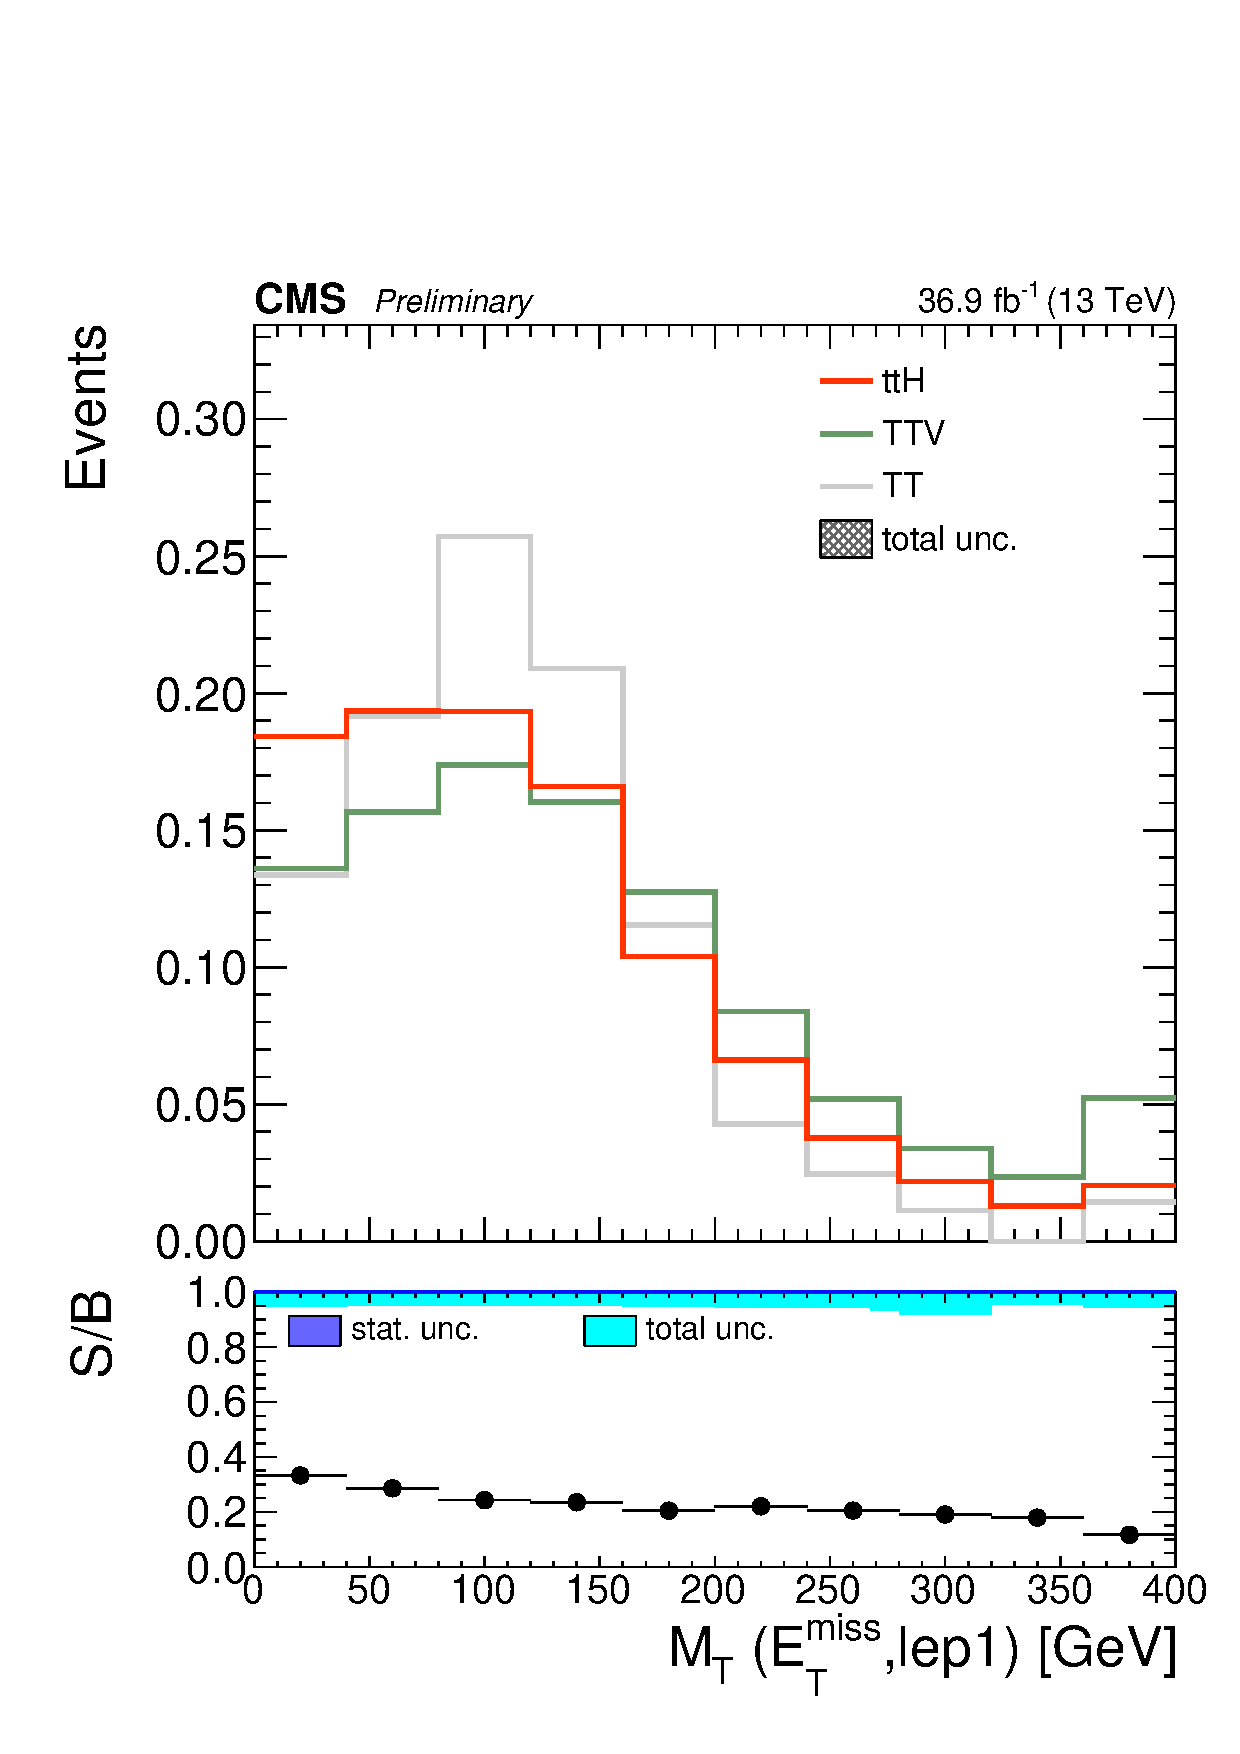
\includegraphics[width=0.32\textwidth]{plots_extraction/training/3l/kinMVA_input_MT_met_lep1.pdf}\\
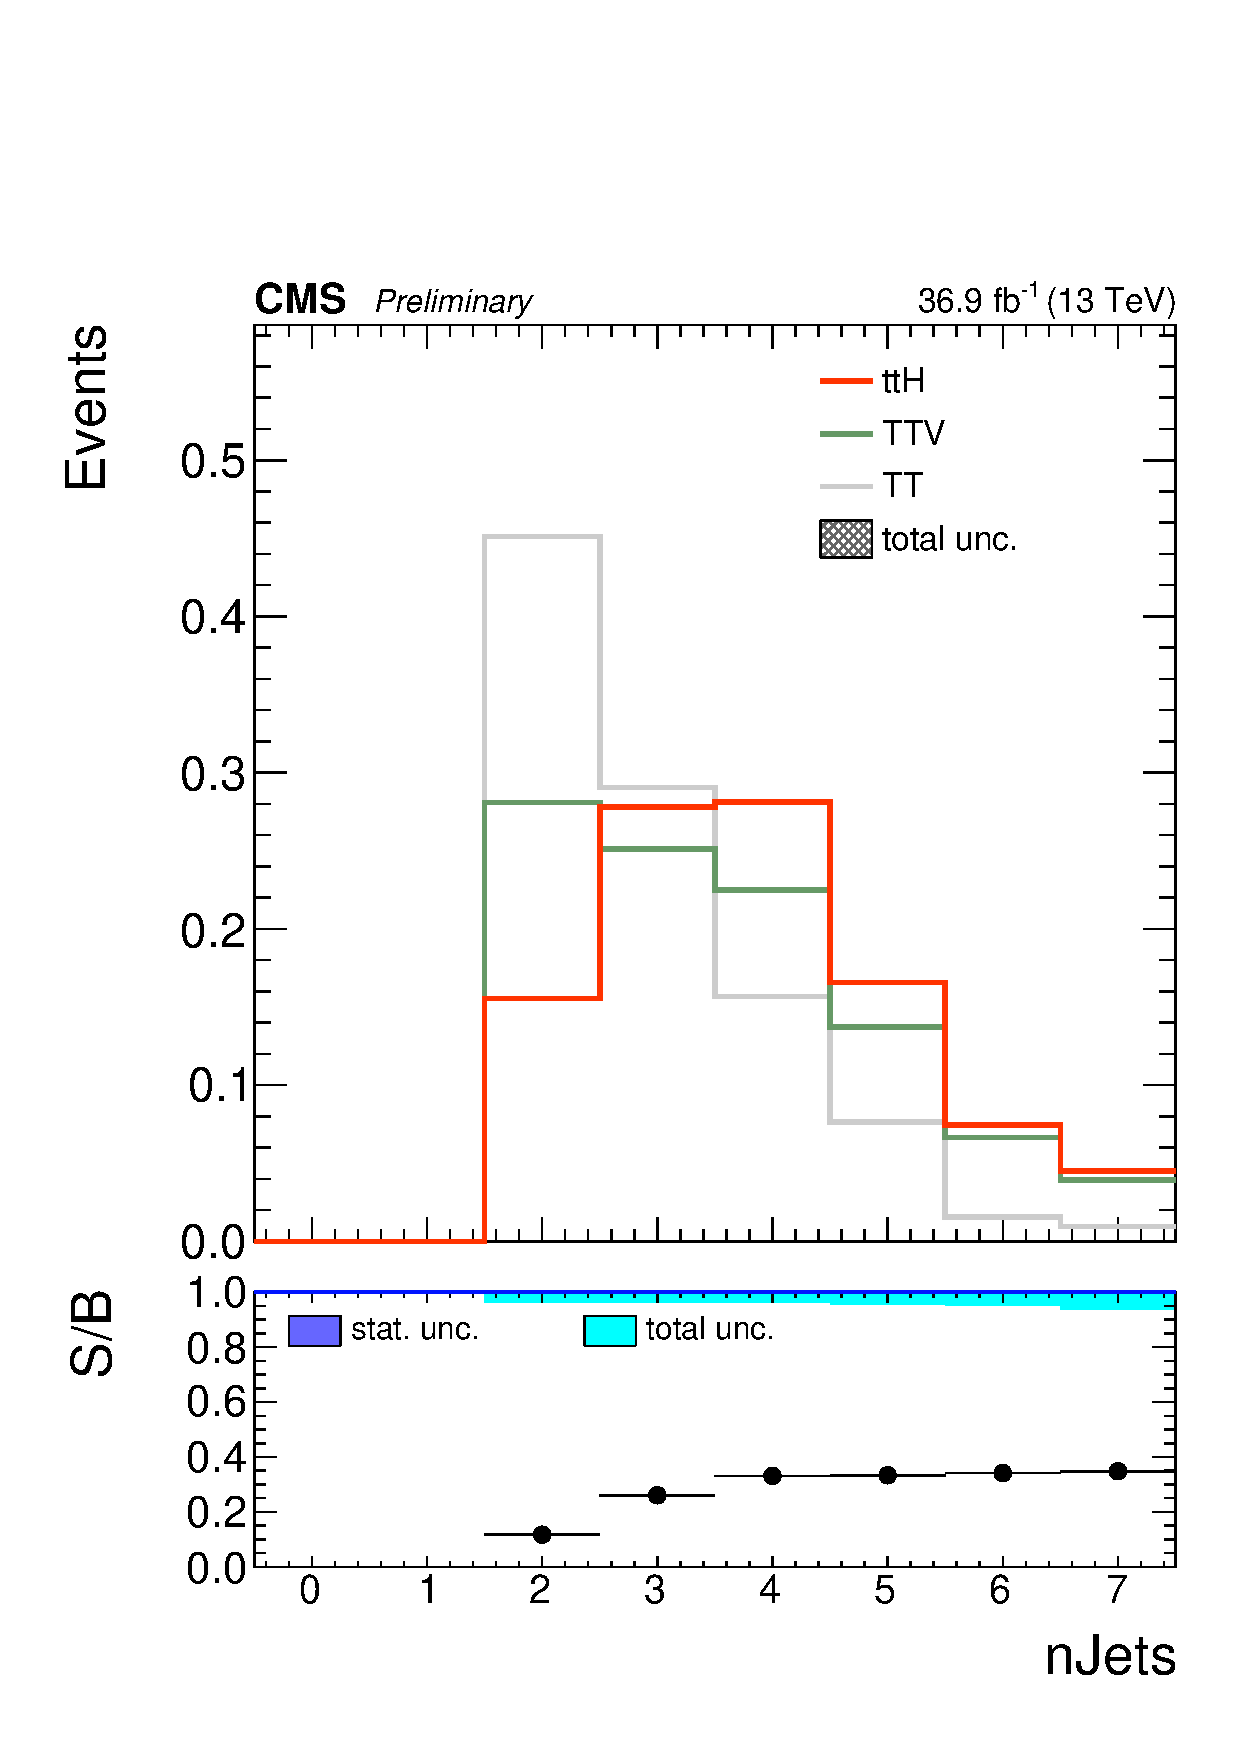
\includegraphics[width=0.32\textwidth]{plots_extraction/training/3l/kinMVA_input_numJets.pdf}
%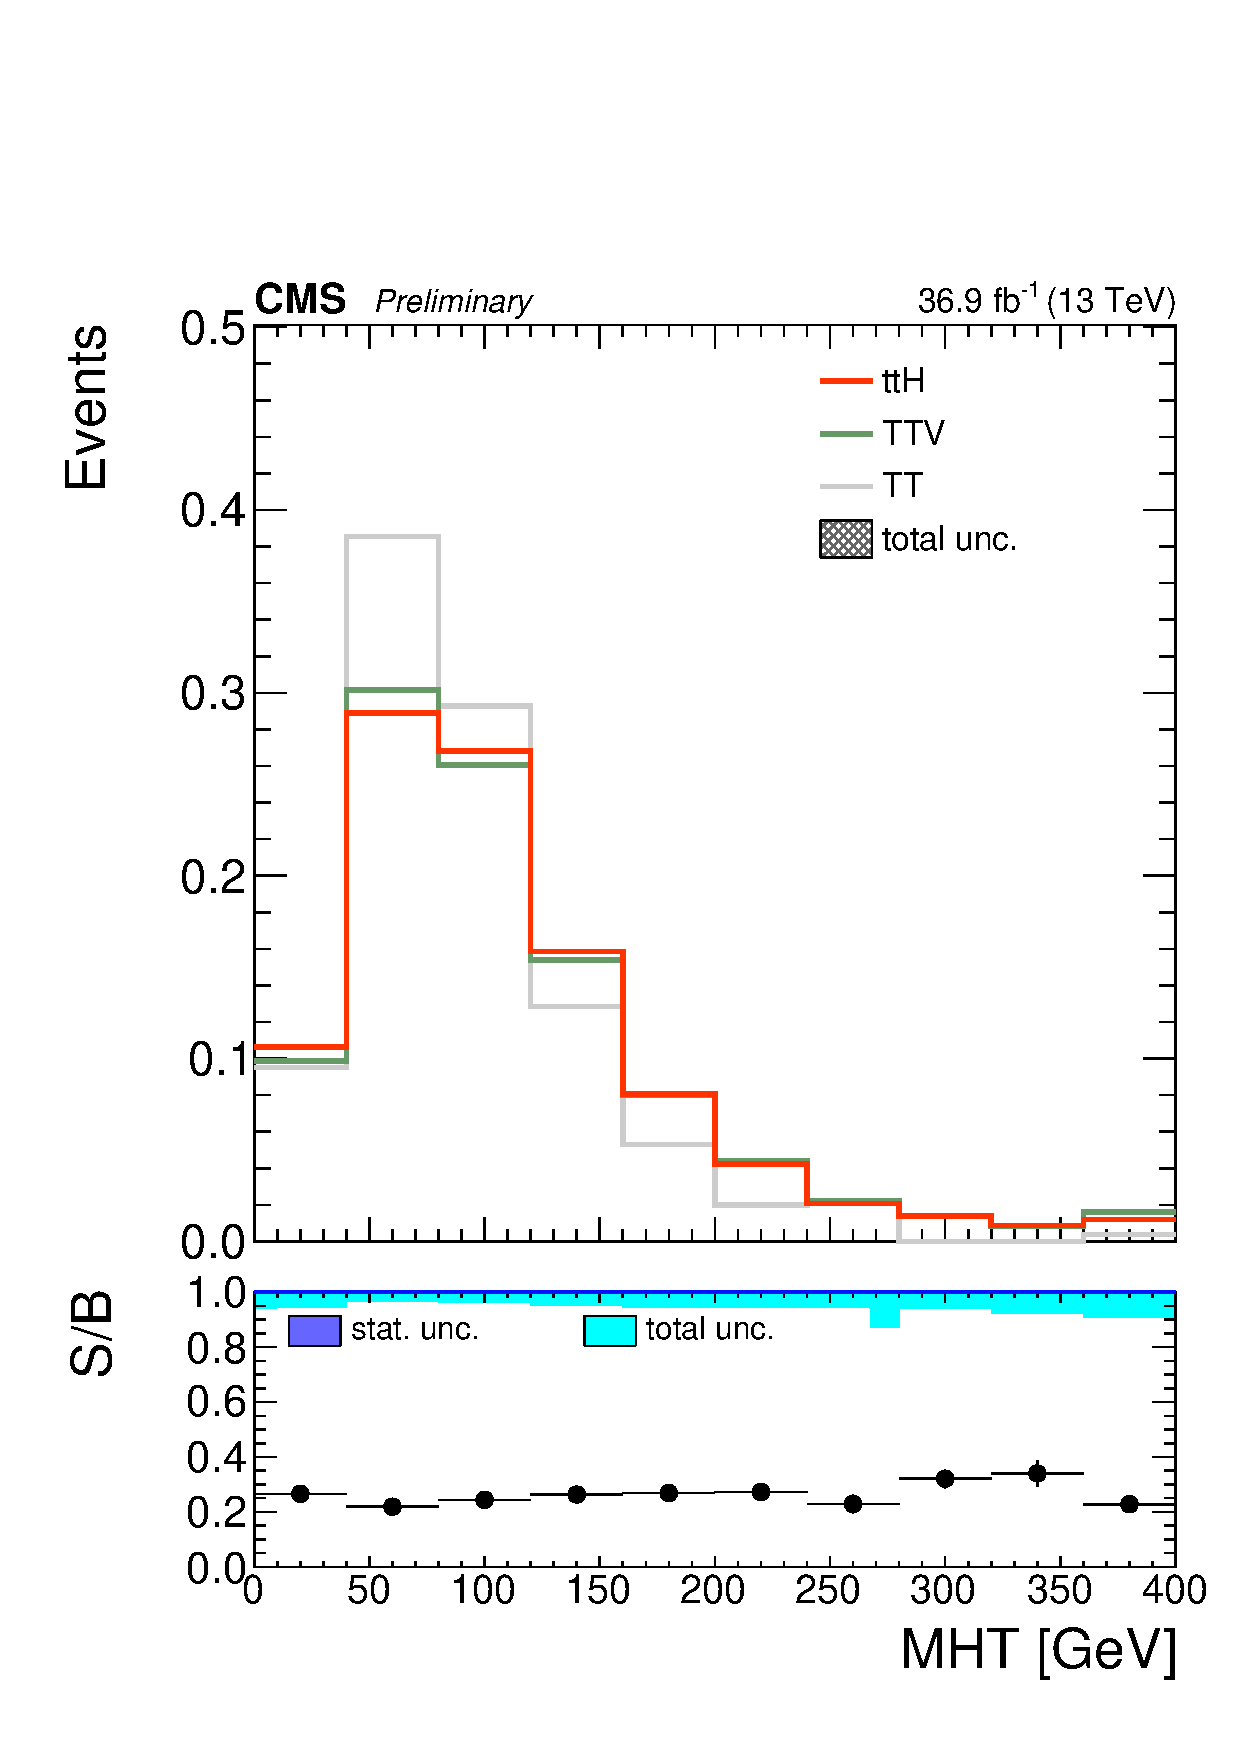
\includegraphics[width=0.32\textwidth]{plots_extraction/training/3l/kinMVA_input_mhtJet25.pdf}
%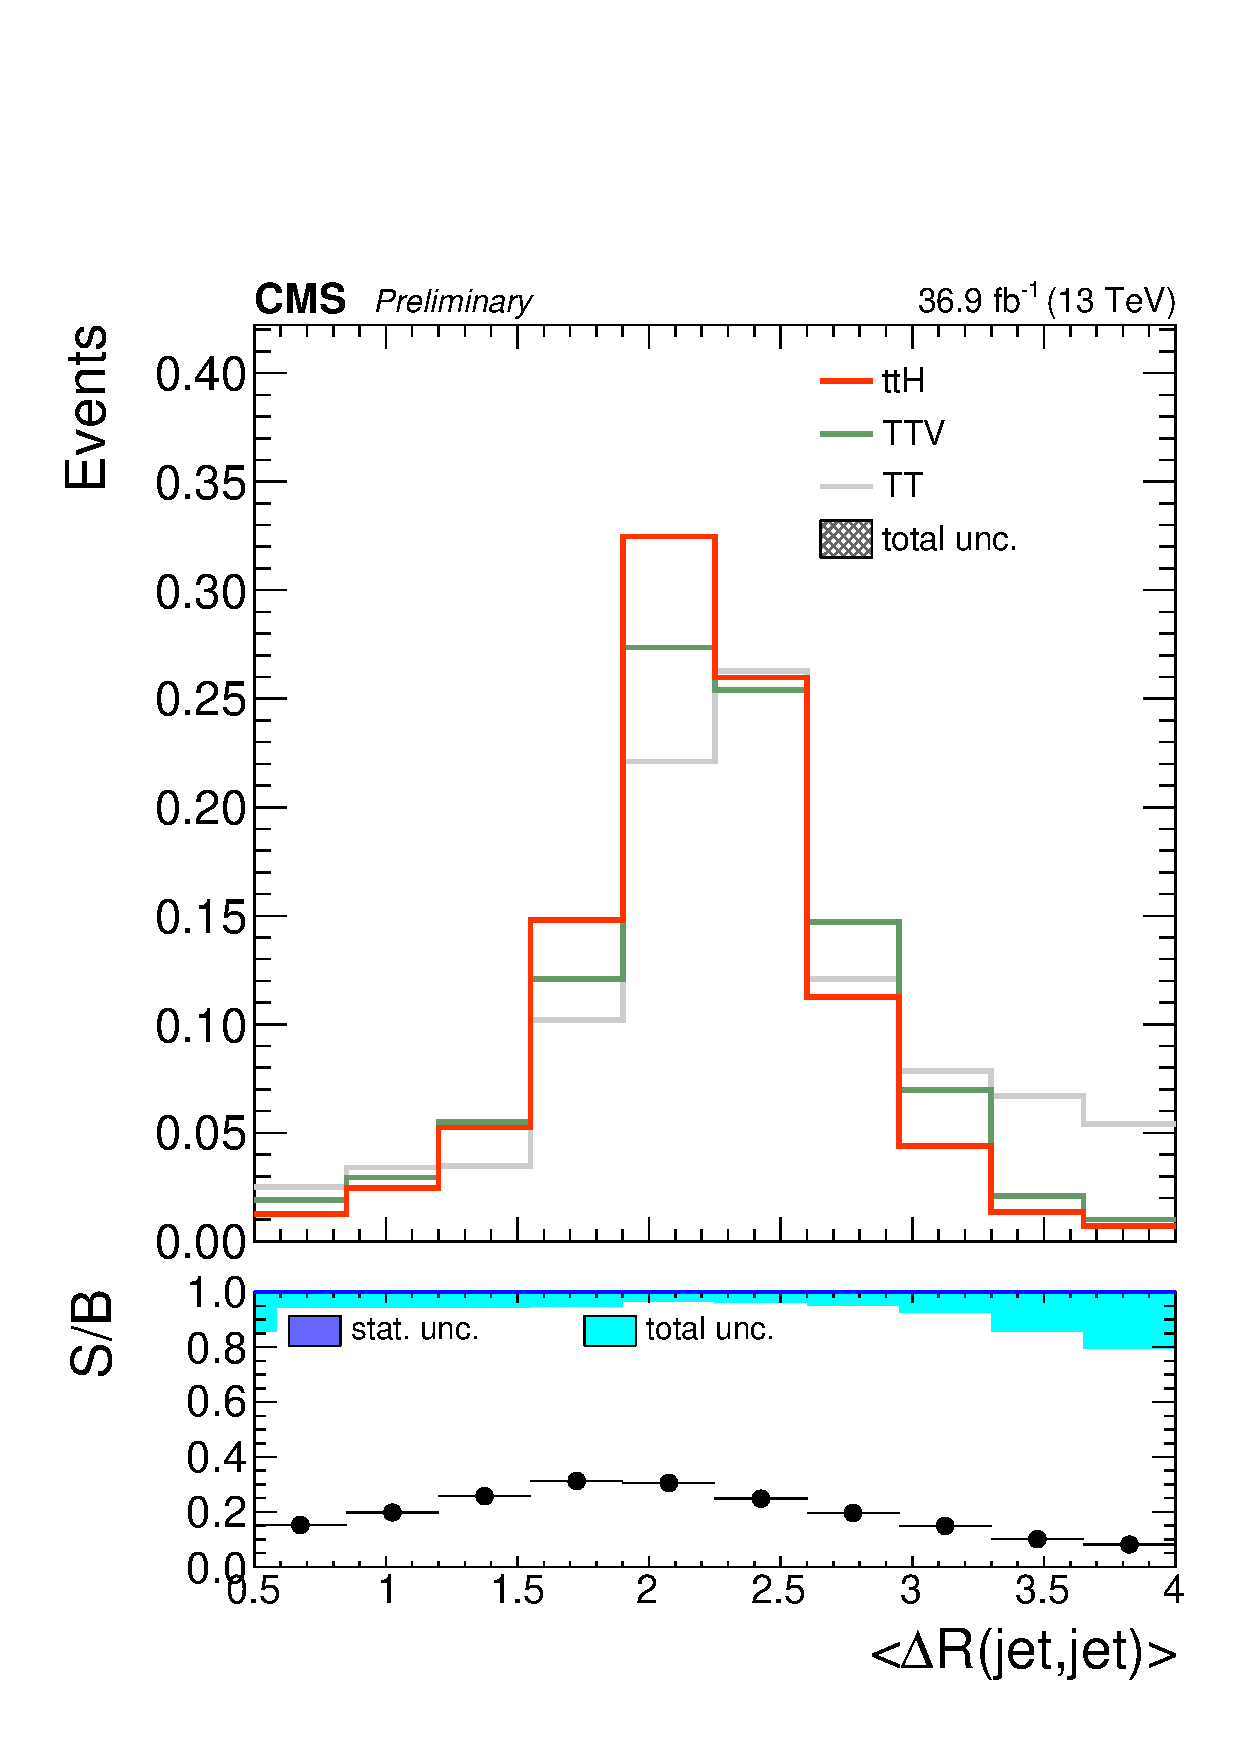
\includegraphics[width=0.32\textwidth]{plots_extraction/training/3l/kinMVA_input_avg_dr_jet.pdf}
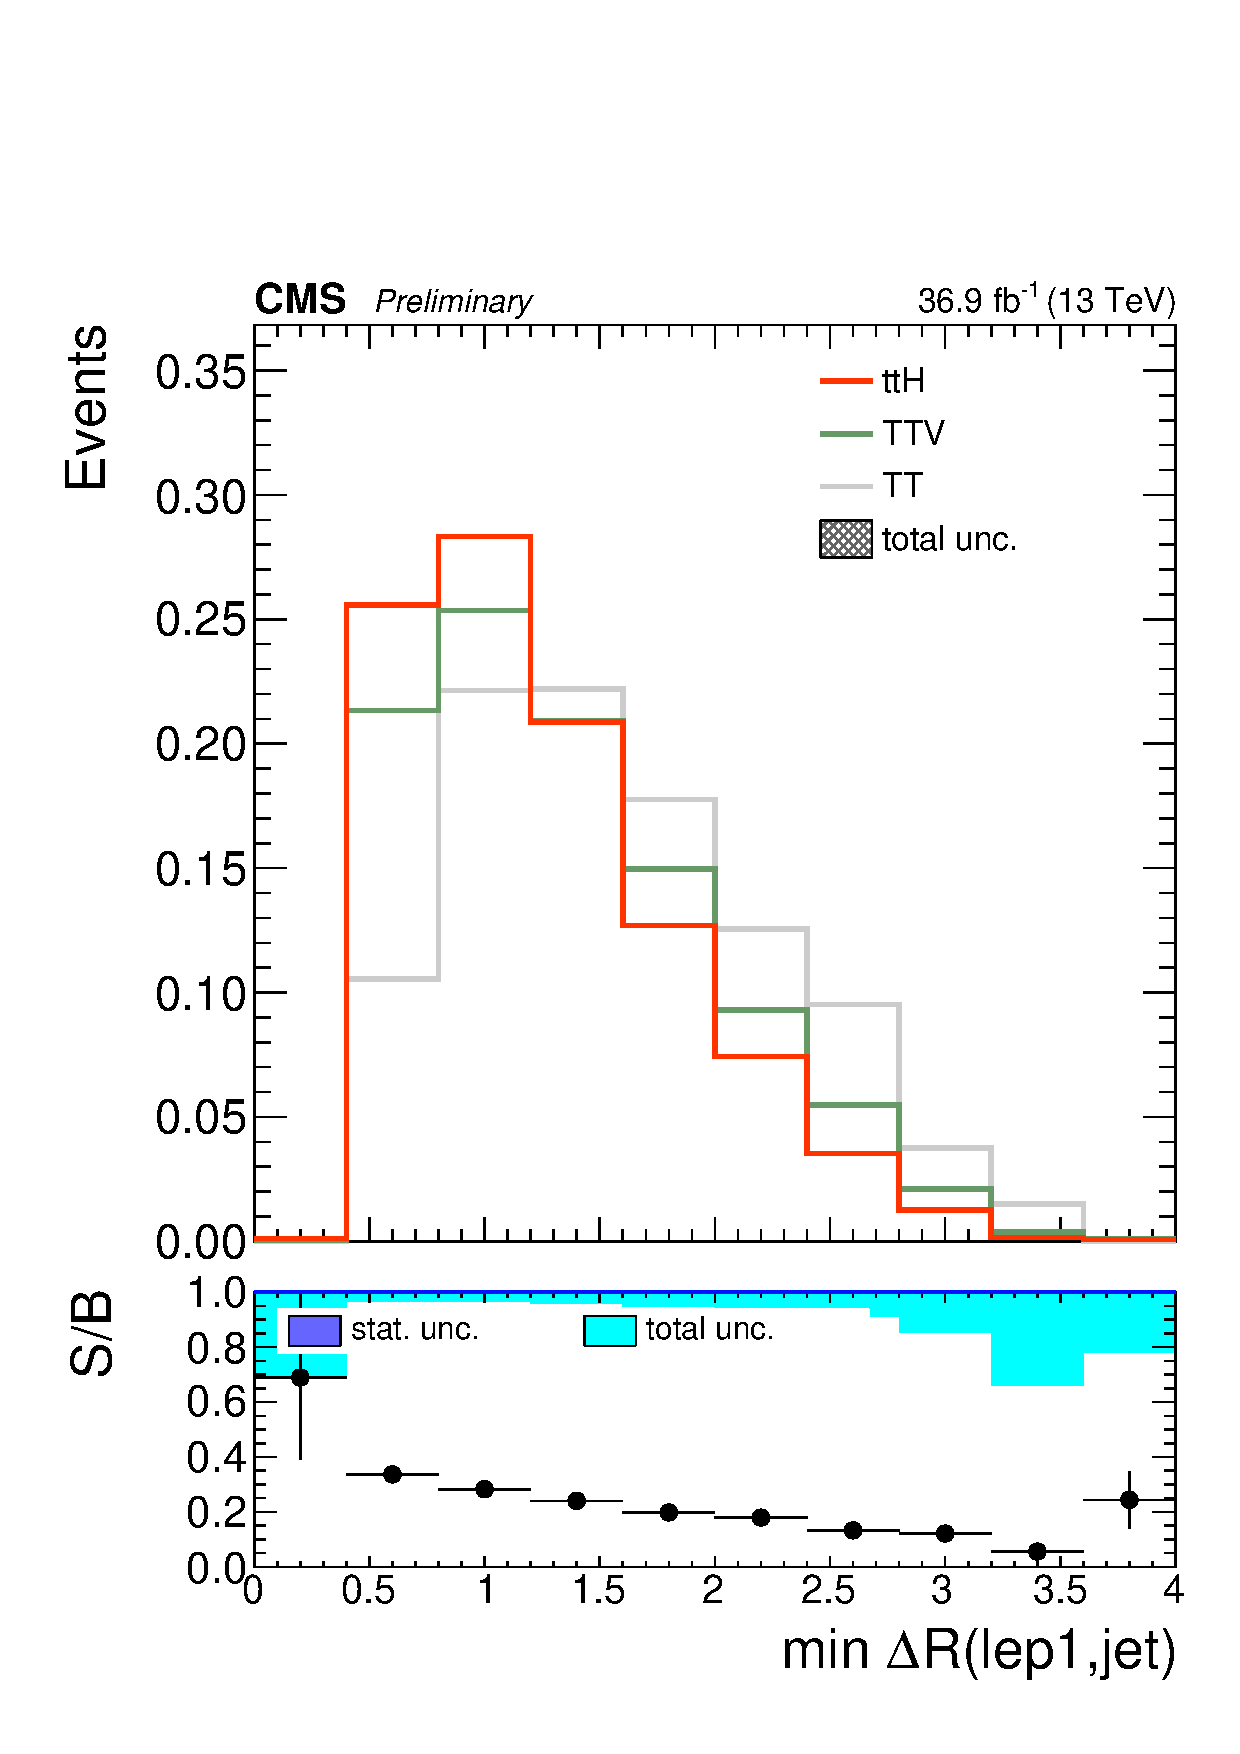
\includegraphics[width=0.32\textwidth]{plots_extraction/training/3l/kinMVA_input_mindr_lep1_jet.pdf}
        \caption{The separation power of the variables used for BDT trainings, in the three lepton channel.}
        \label{fig:3l_training_1}
\end{figure}

\begin{figure}[htb]
        \centering
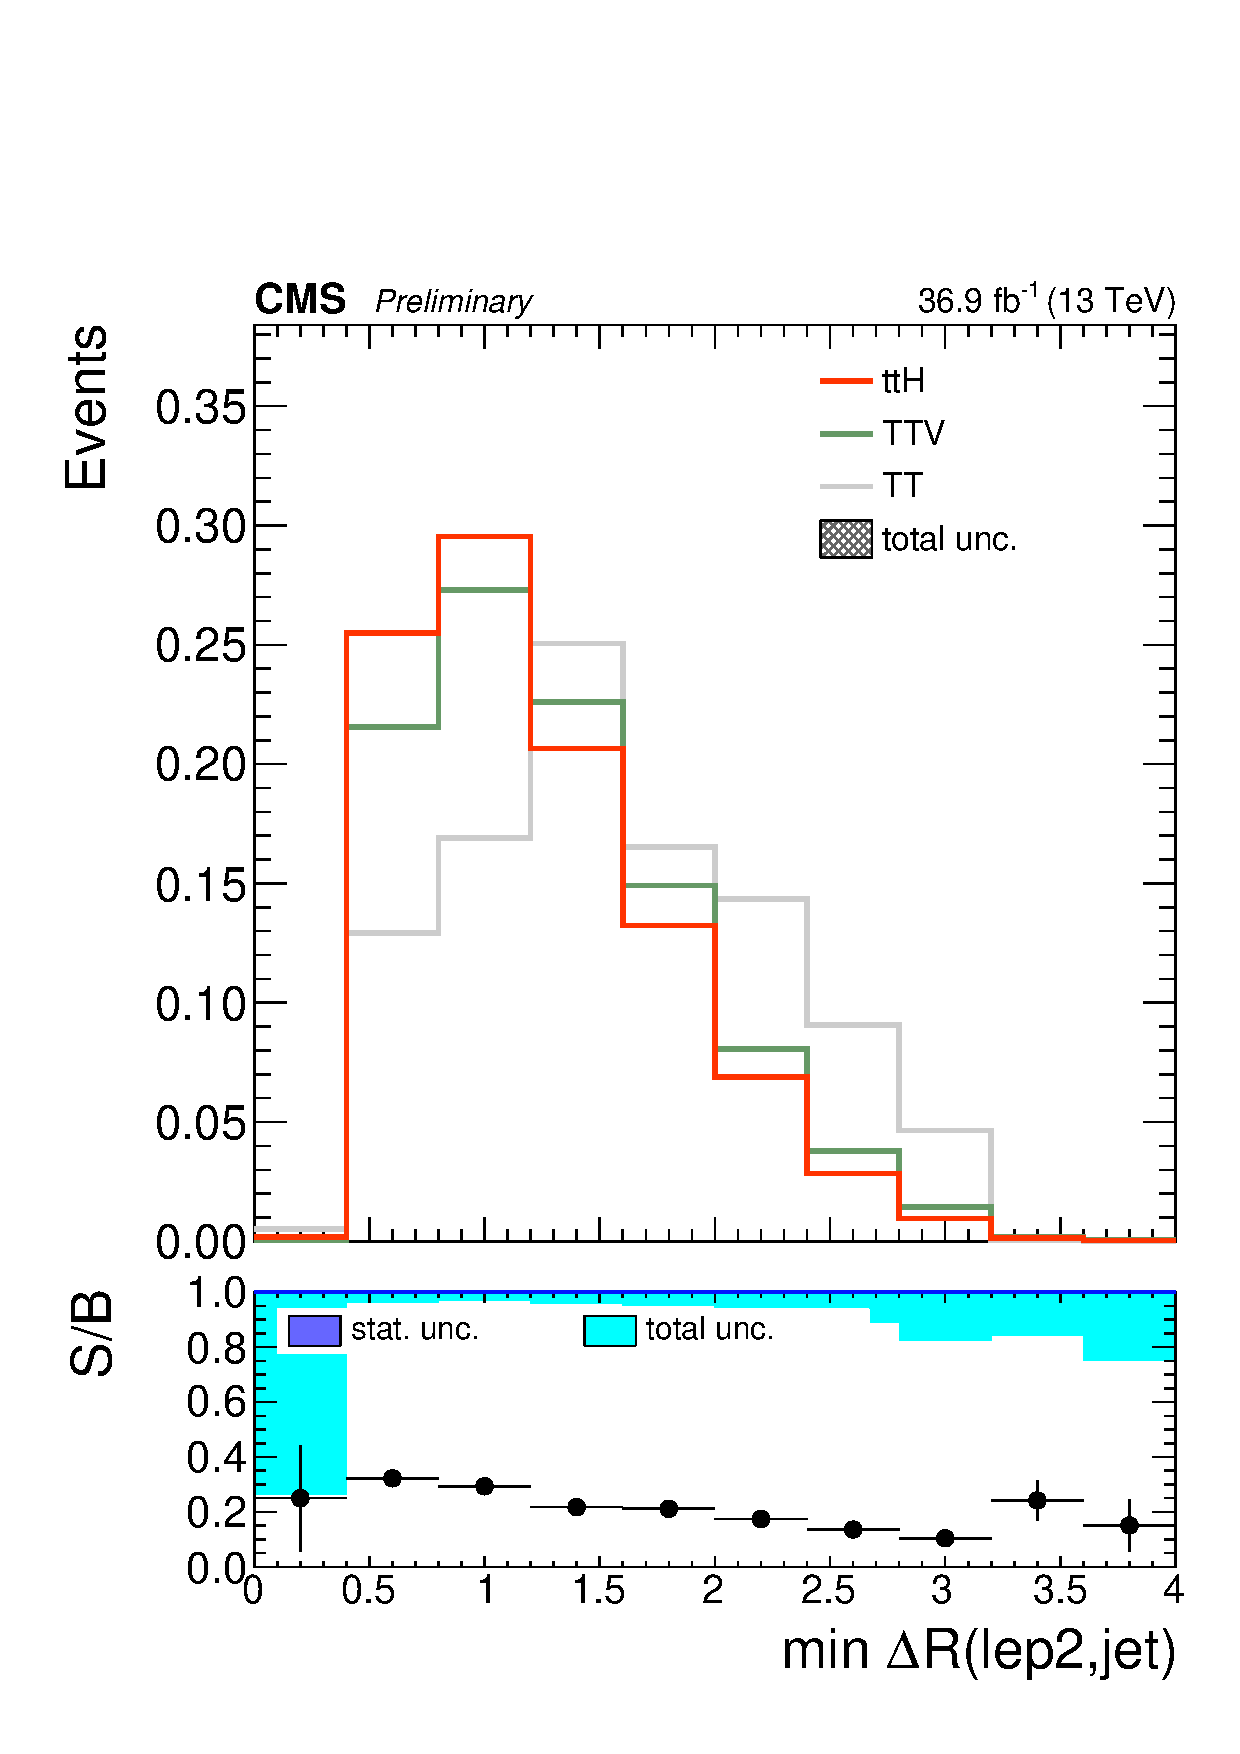
\includegraphics[width=0.32\textwidth]{plots_extraction/training/3l/kinMVA_input_mindr_lep2_jet.pdf}
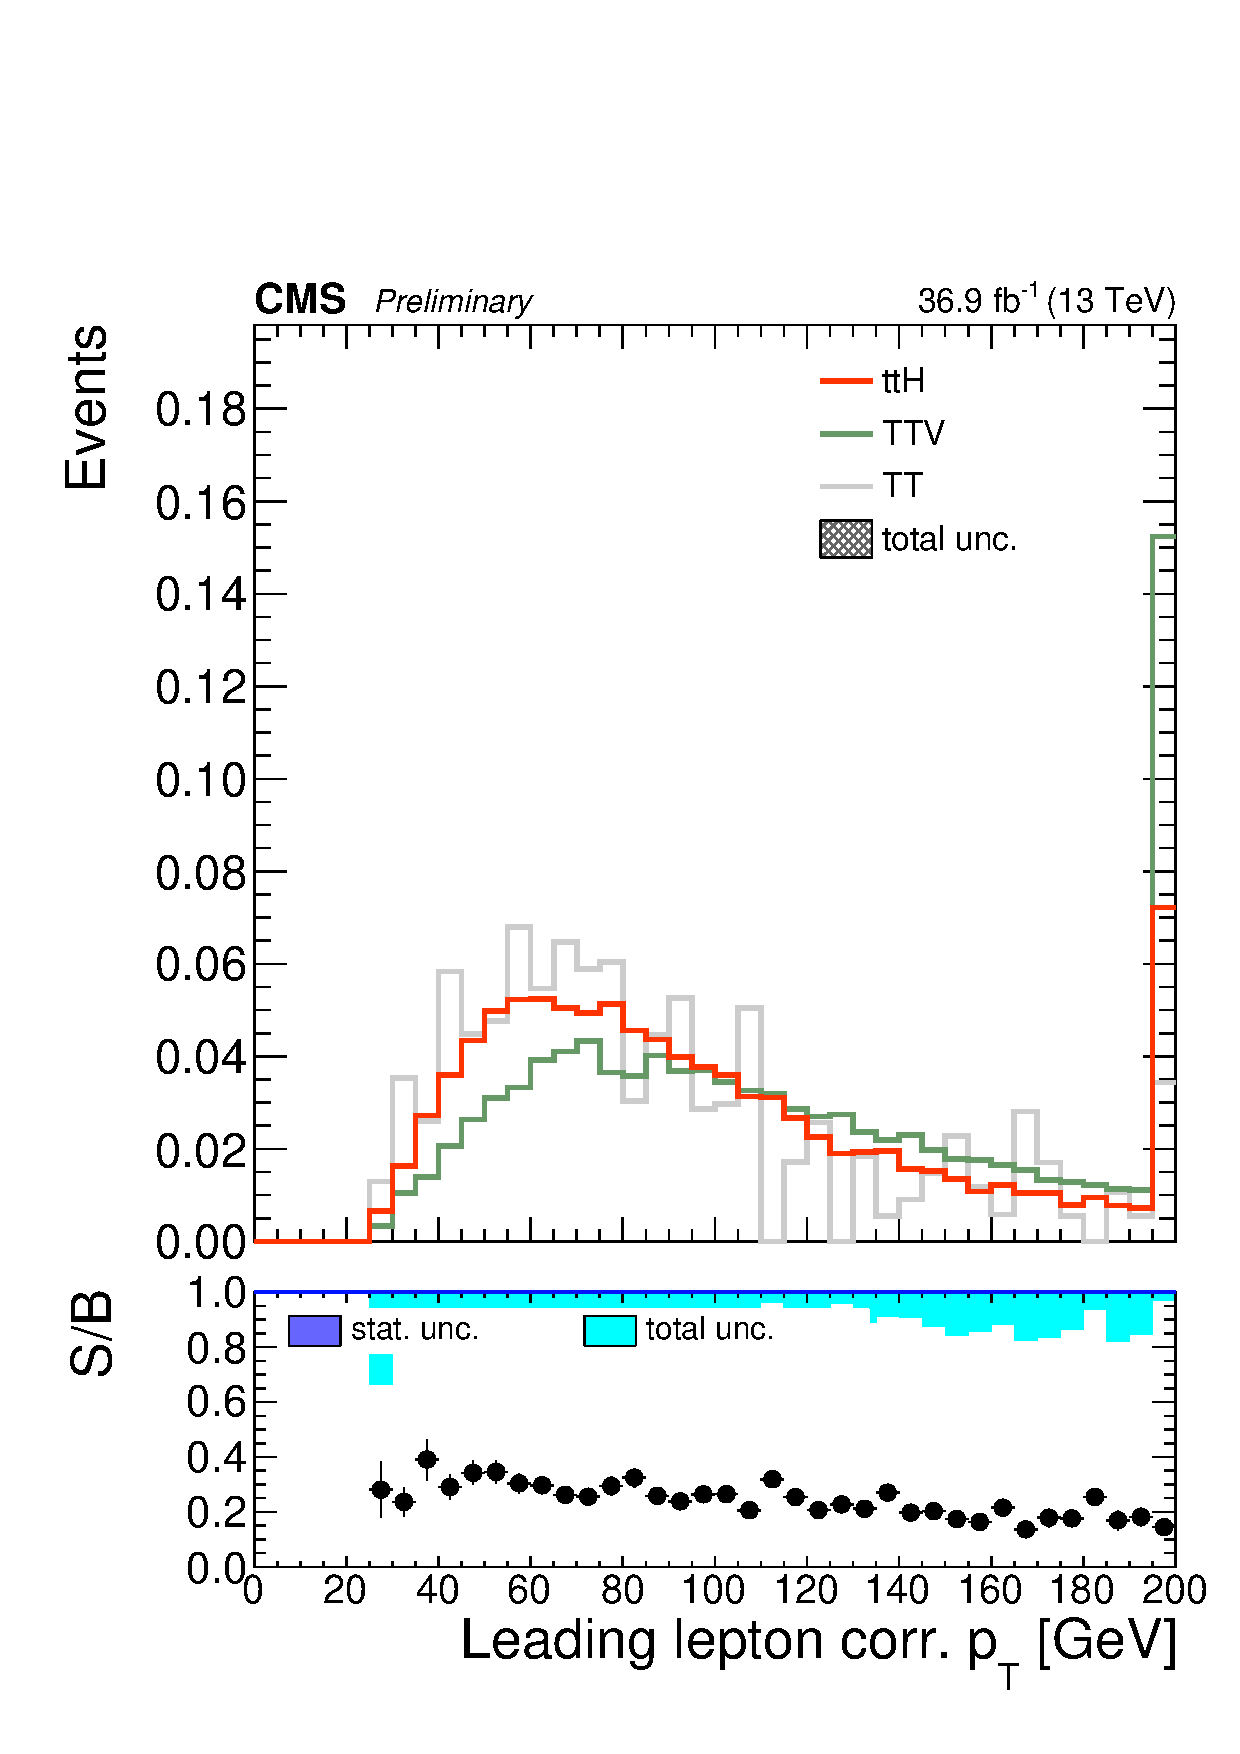
\includegraphics[width=0.32\textwidth]{plots_extraction/training/3l/kinMVA_input_LepGood0_conePt.pdf}
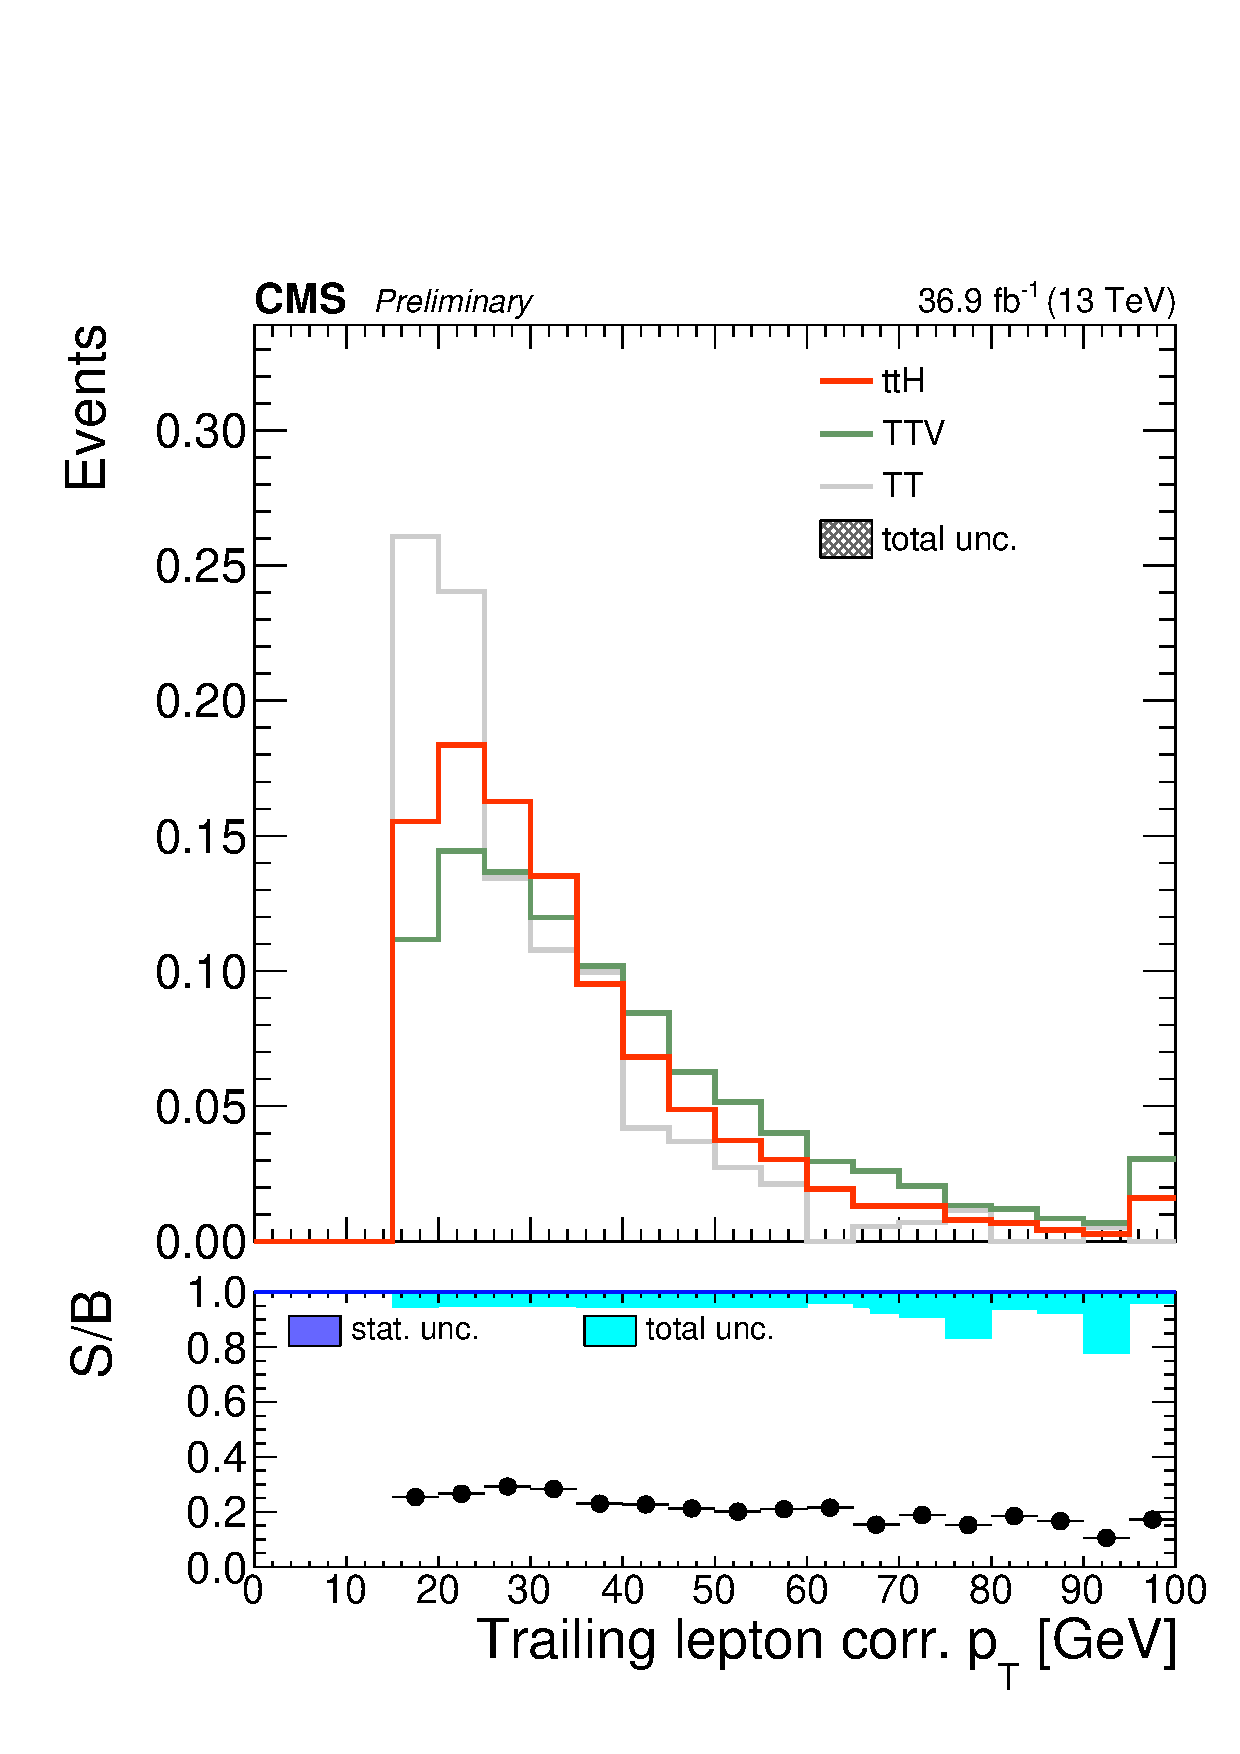
\includegraphics[width=0.32\textwidth]{plots_extraction/training/3l/kinMVA_input_LepGood2_conePt.pdf}\\
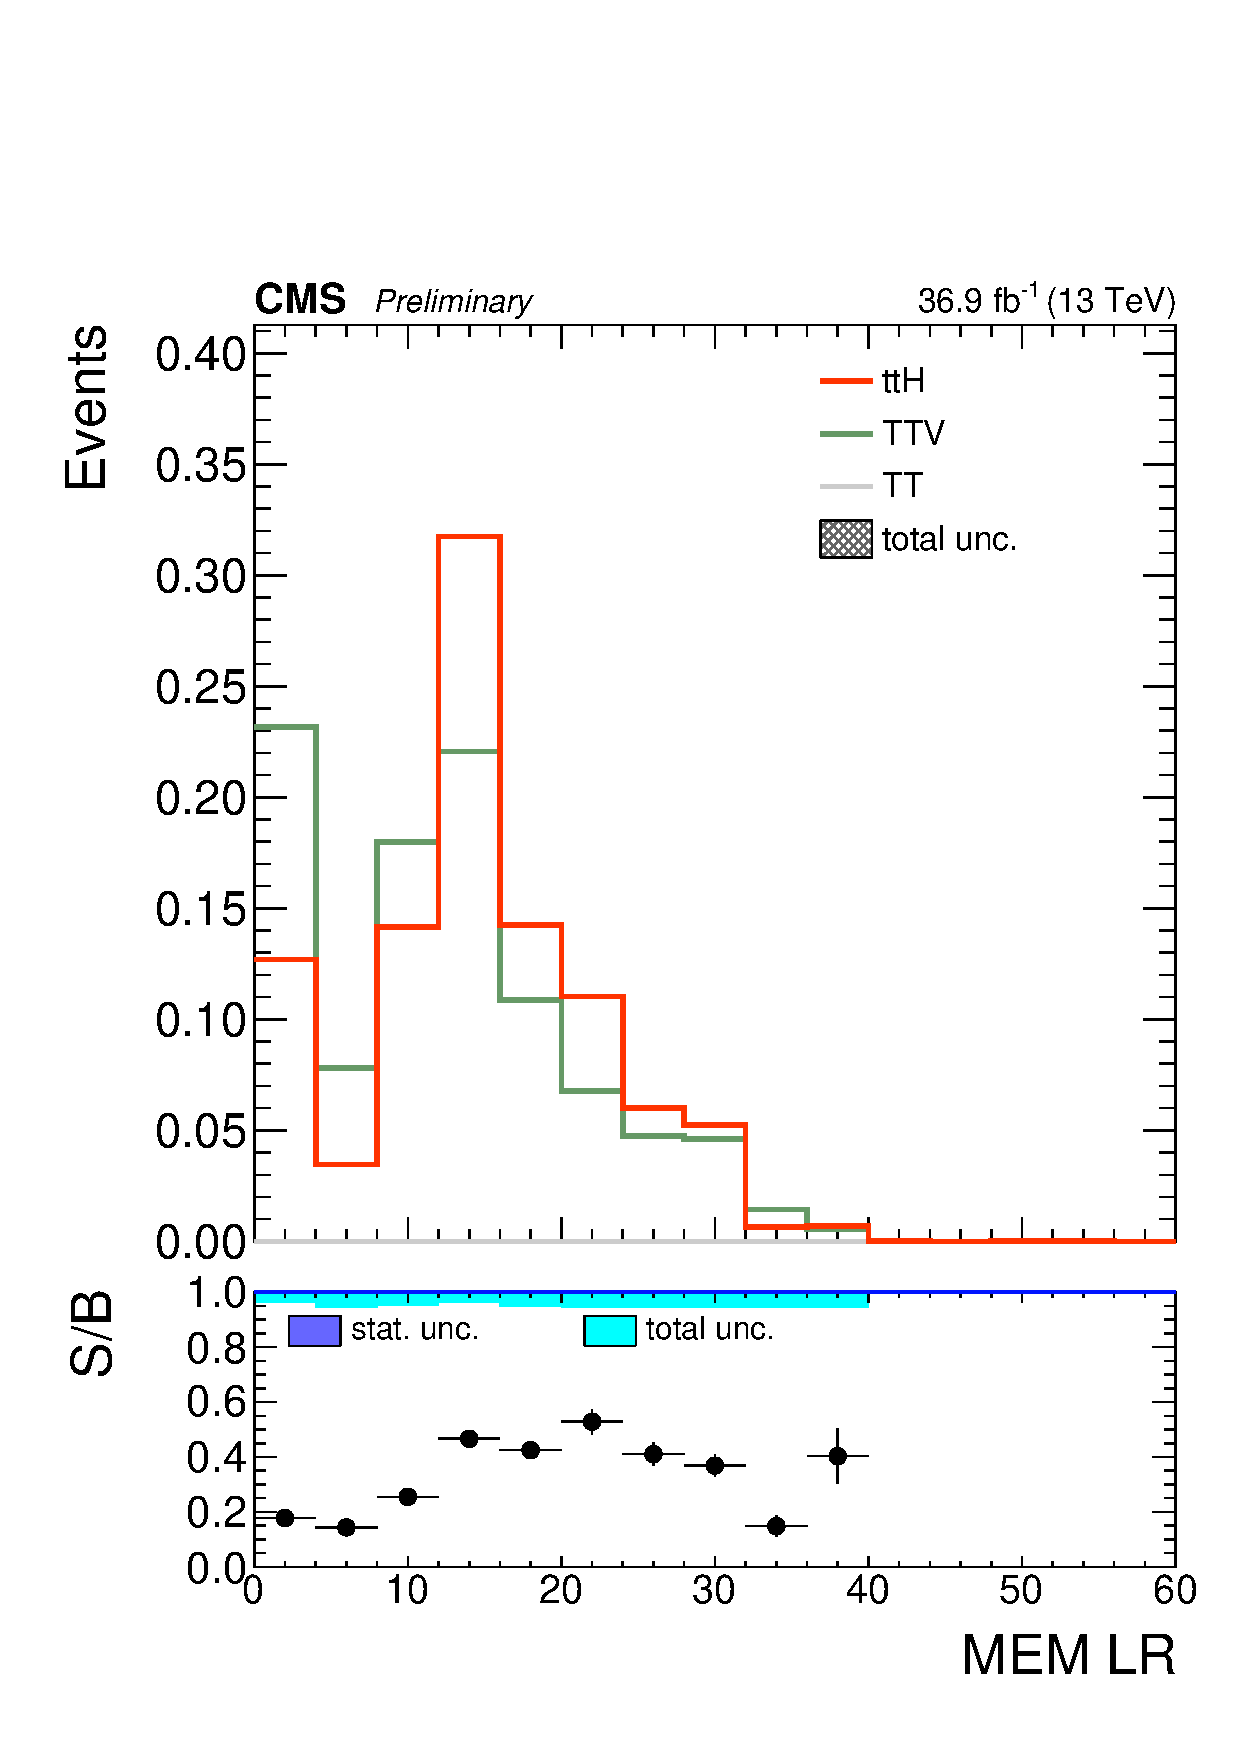
\includegraphics[width=0.32\textwidth]{plots_extraction/training/3l/kinMVA_input_MEM_LR.pdf}
%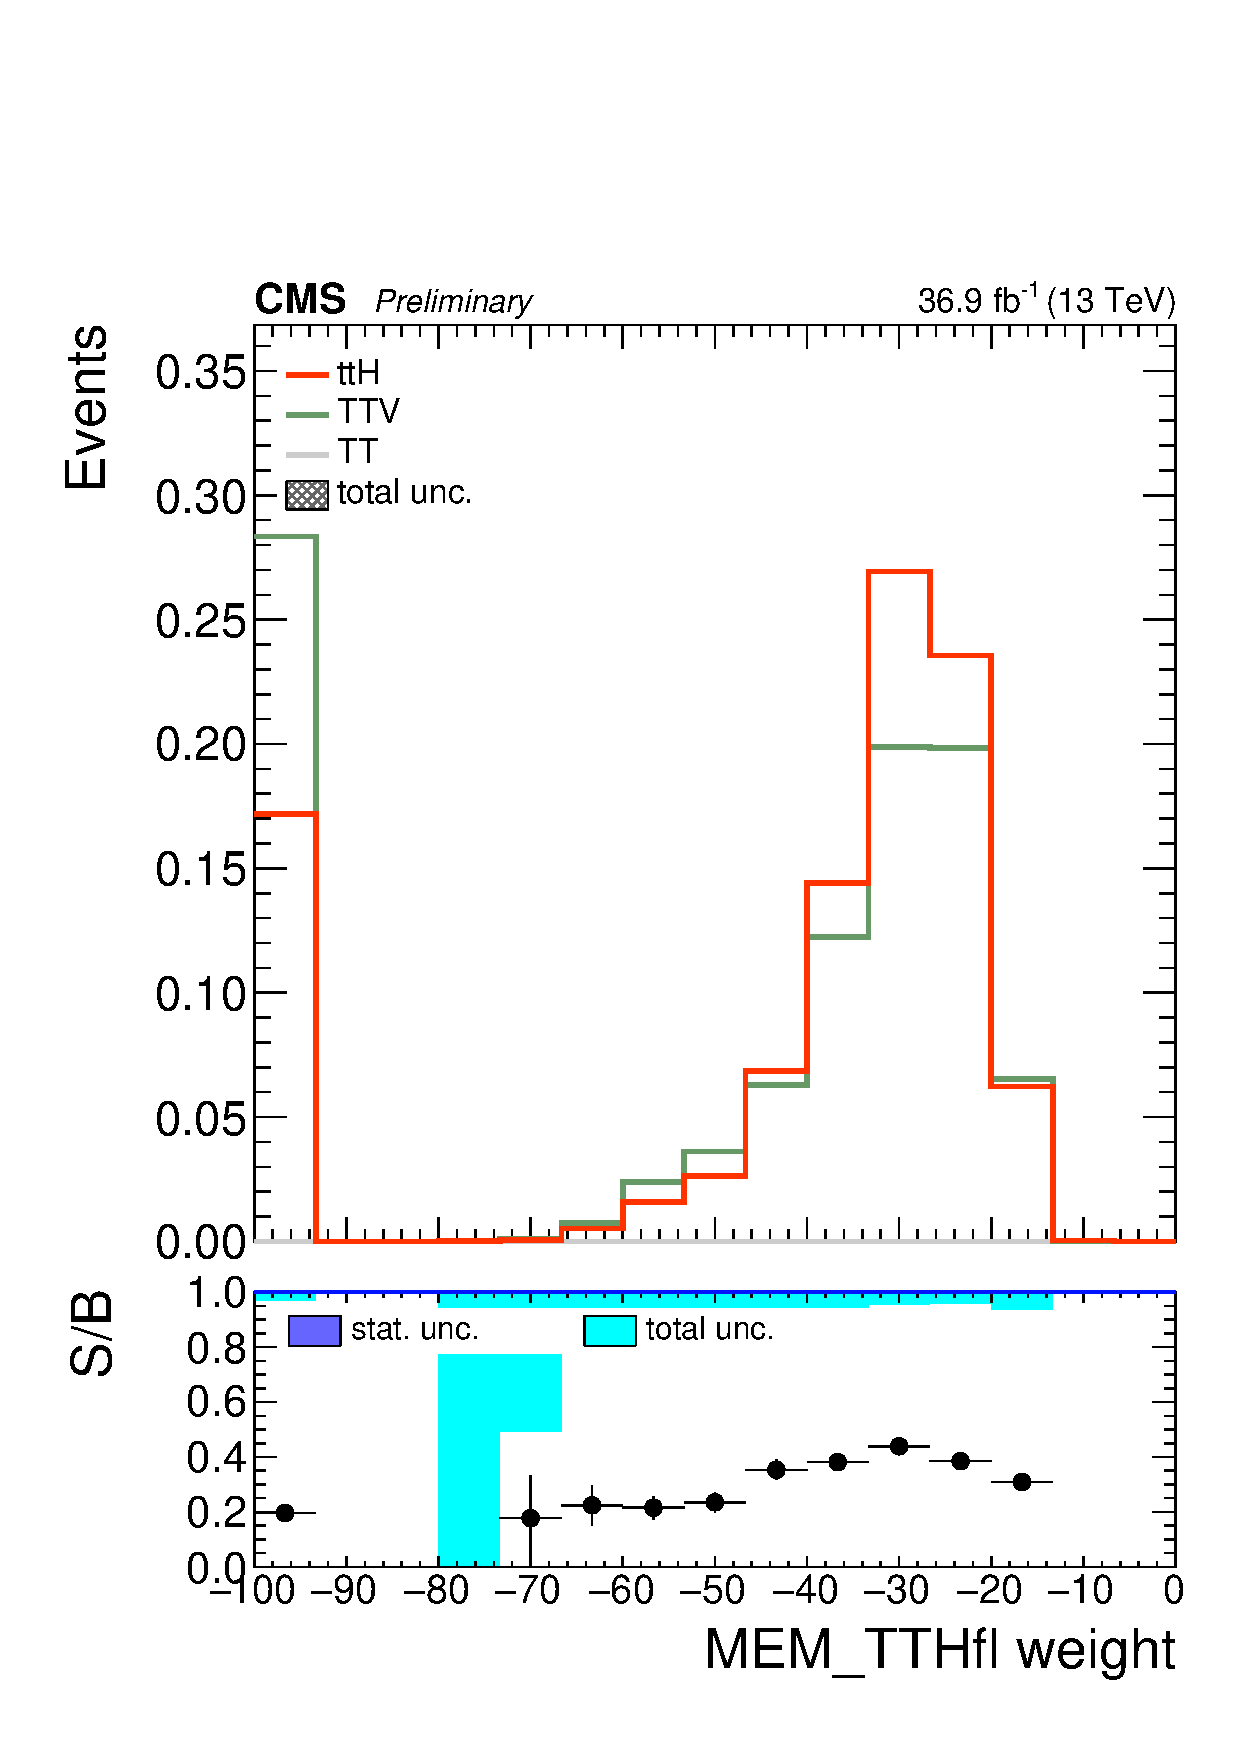
\includegraphics[width=0.32\textwidth]{plots_extraction/training/3l/kinMVA_input_MEM_TTHfl.pdf}
%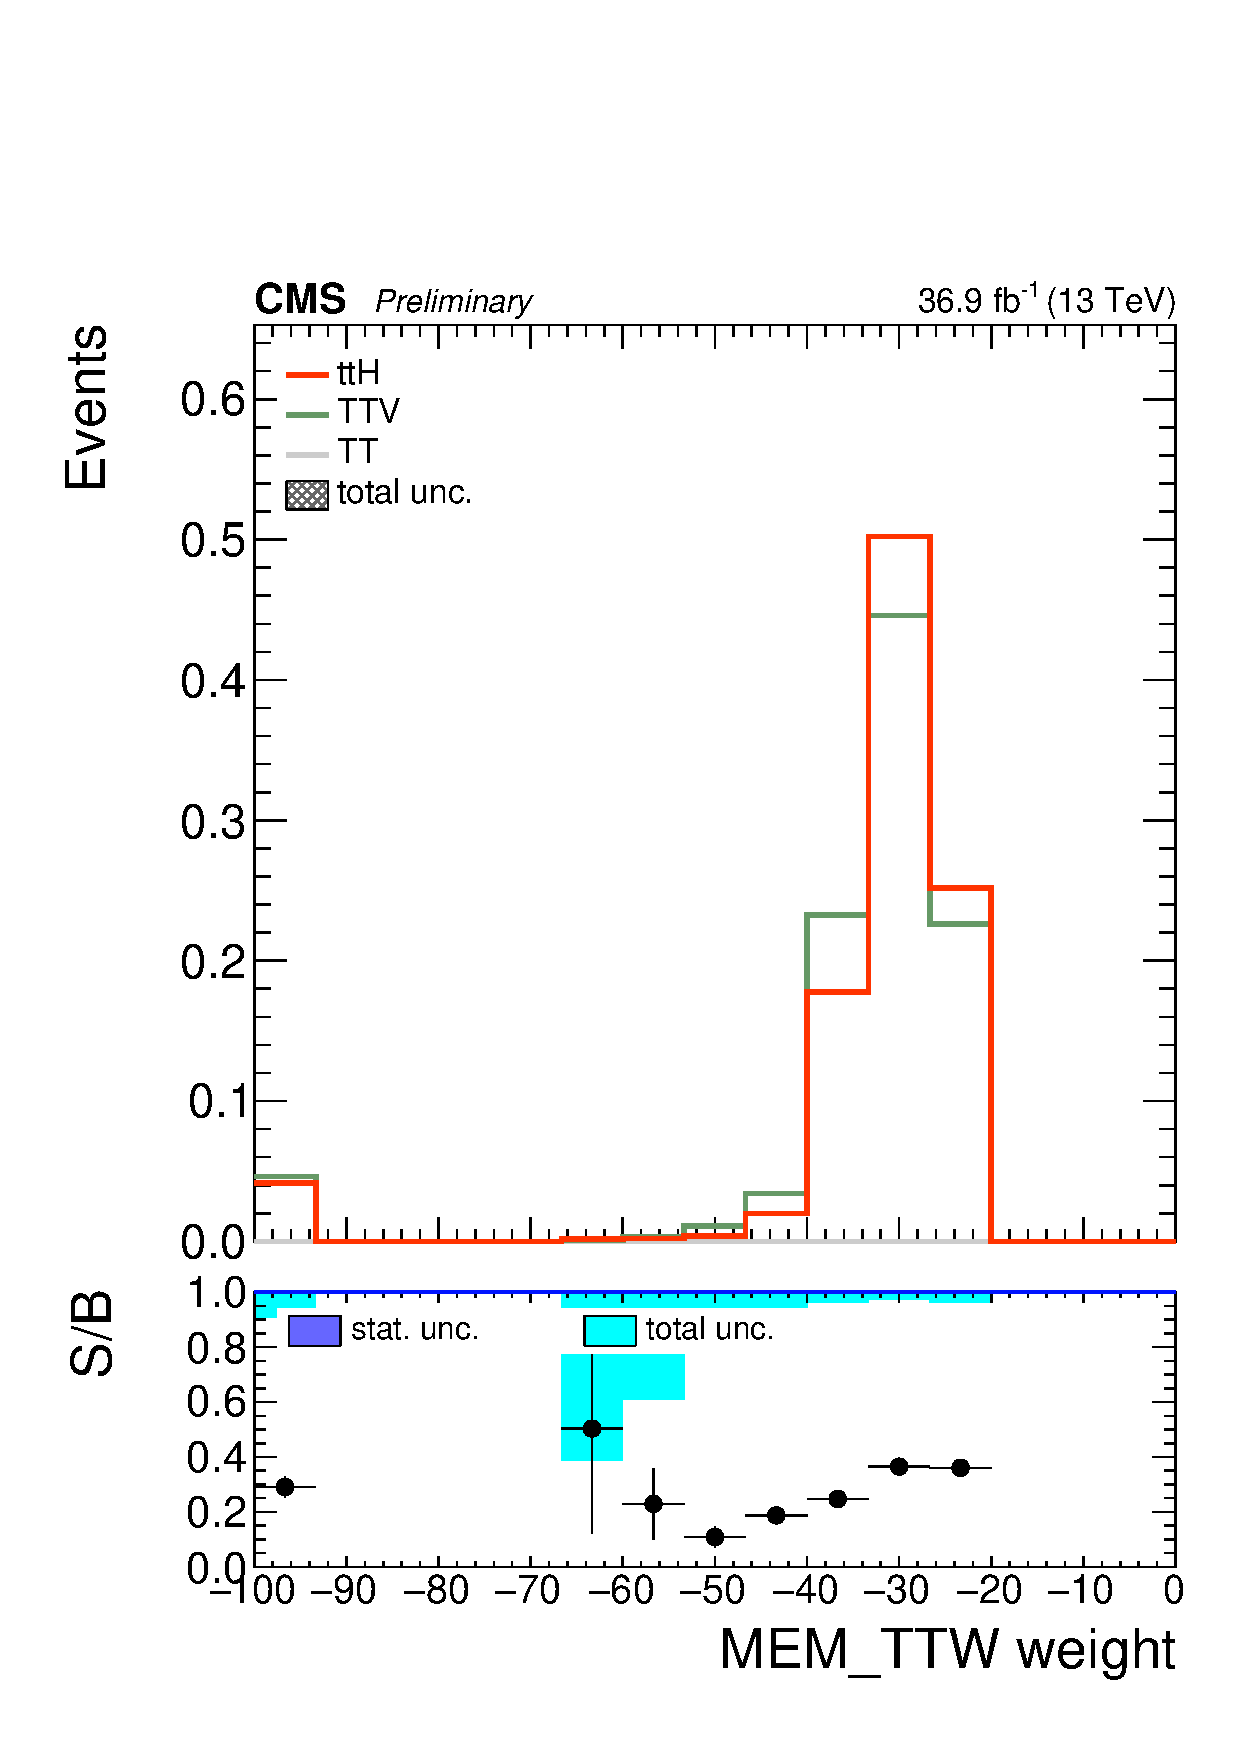
\includegraphics[width=0.32\textwidth]{plots_extraction/training/3l/kinMVA_input_MEM_TTW.pdf}
%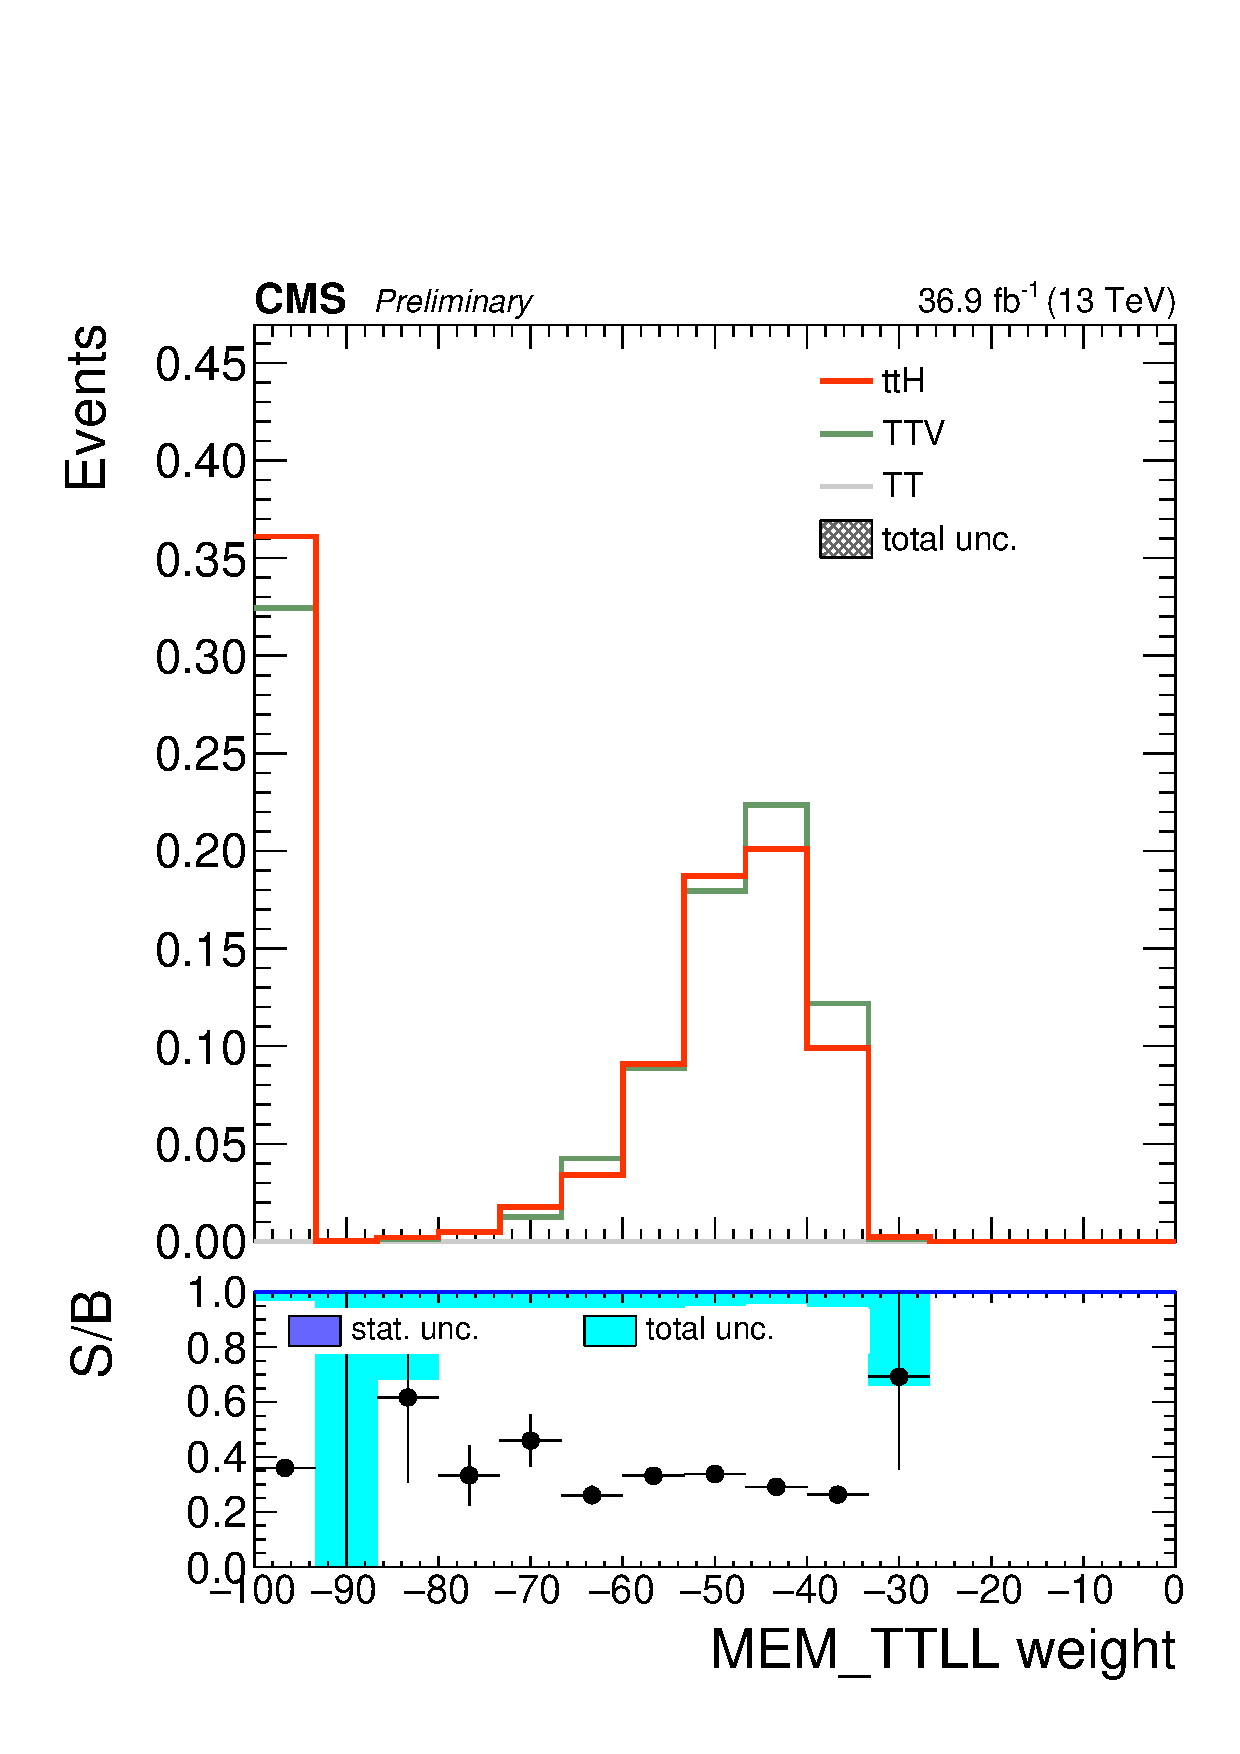
\includegraphics[width=0.32\textwidth]{plots_extraction/training/3l/kinMVA_input_MEM_TTLL.pdf}
        \caption{The separation power of the variables used for BDT trainings, in the three lepton channel.}
        \label{fig:3l_training_2}
\end{figure}

Figure \ref{fig:3l_mvaOutput} shows the separation power of the BDT discriminators.
%while \ref{fig:3l_mvaOutput} shows the distributions of these discriminators.

%\begin{figure}[htb]
%        \centering
%%\begin{subfigure}
%	%\centering
%\includegraphics[width=0.35\textwidth]{plots_extraction/training/3l/kinMVA_3l_ttbar.pdf}
%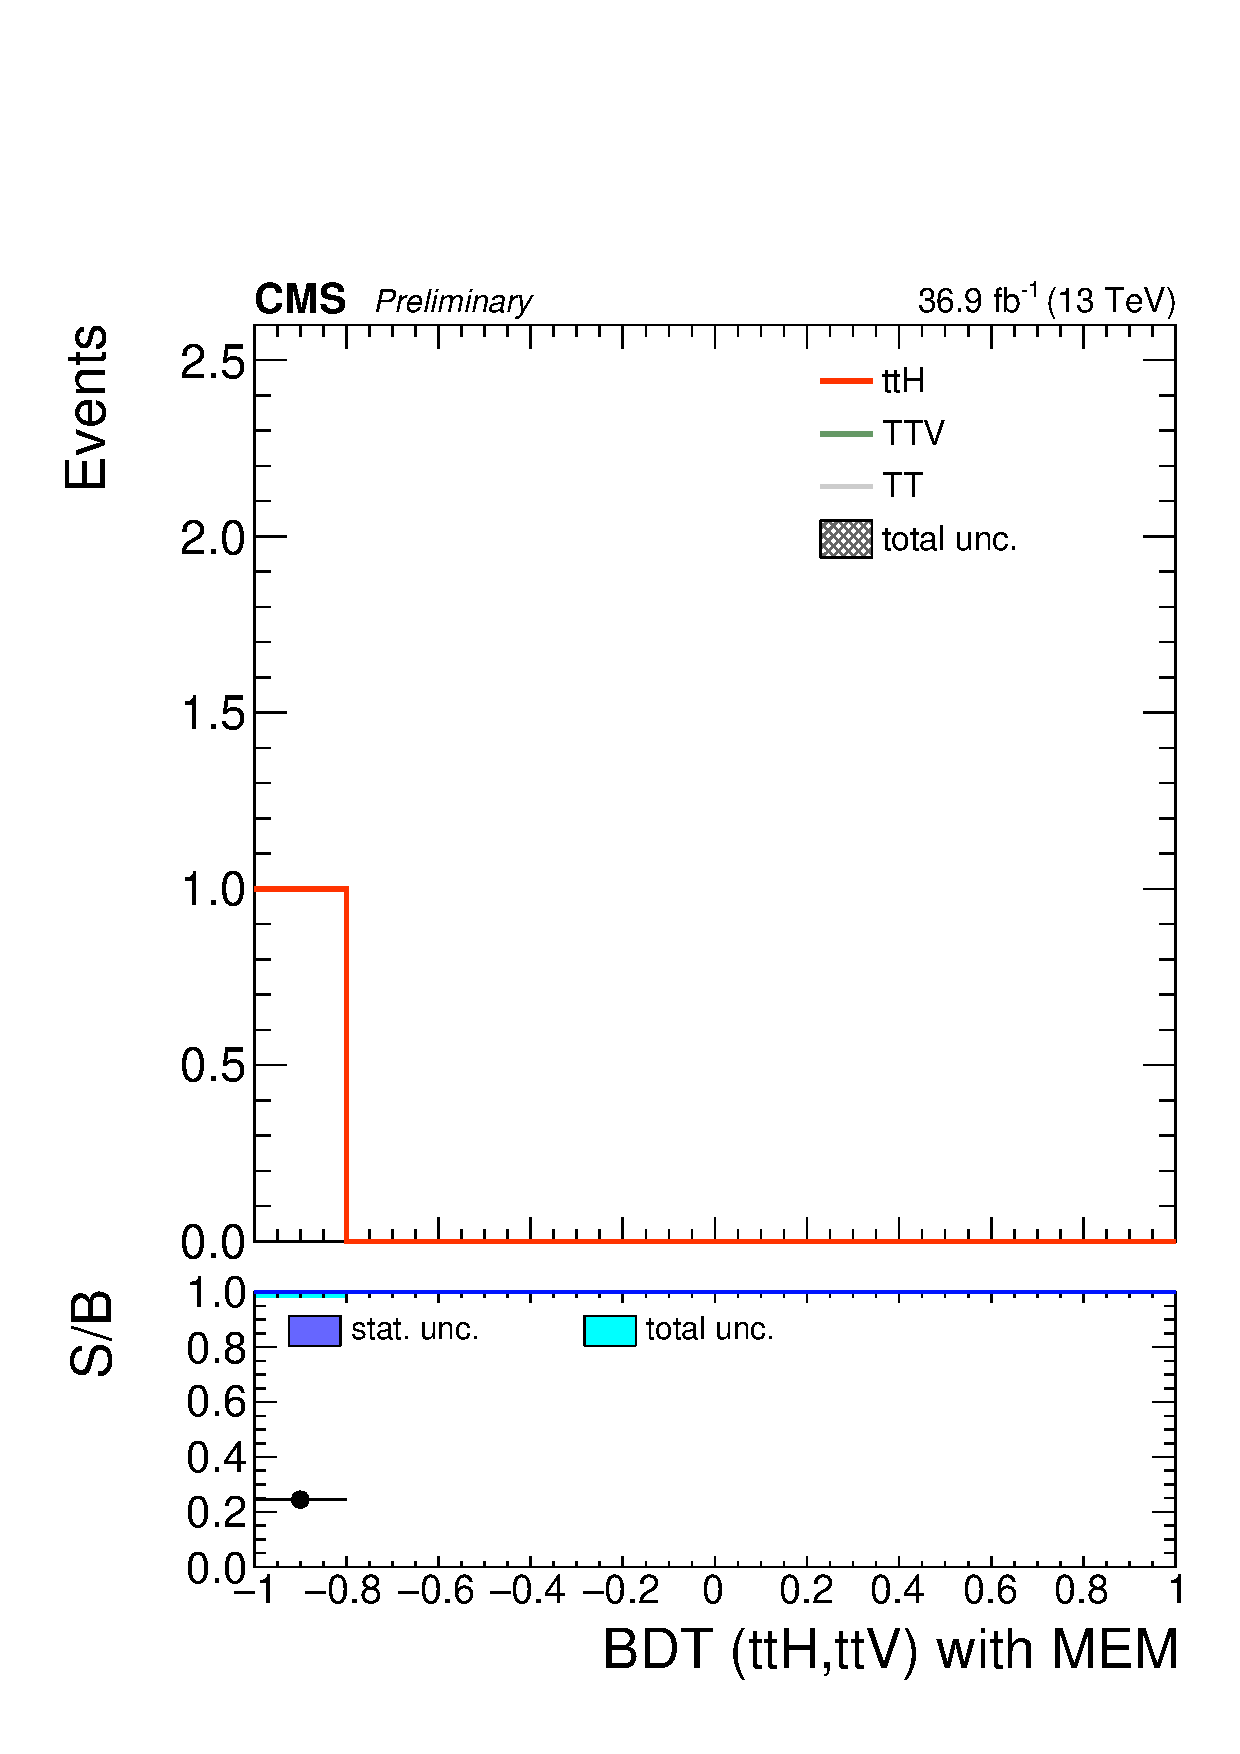
\includegraphics[width=0.35\textwidth]{plots_extraction/training/3l/kinMVA_3l_ttV_withMEM.pdf}
%	\caption{The separation power of the BDT output against the ttbar (left) and ttV (right) background, in the three lepton channel.}
%	\label{fig:3l_mvaTraining}
%%\end{subfigure}
%\end{figure}

\begin{figure}[htb]
        \centering
	%\centering
%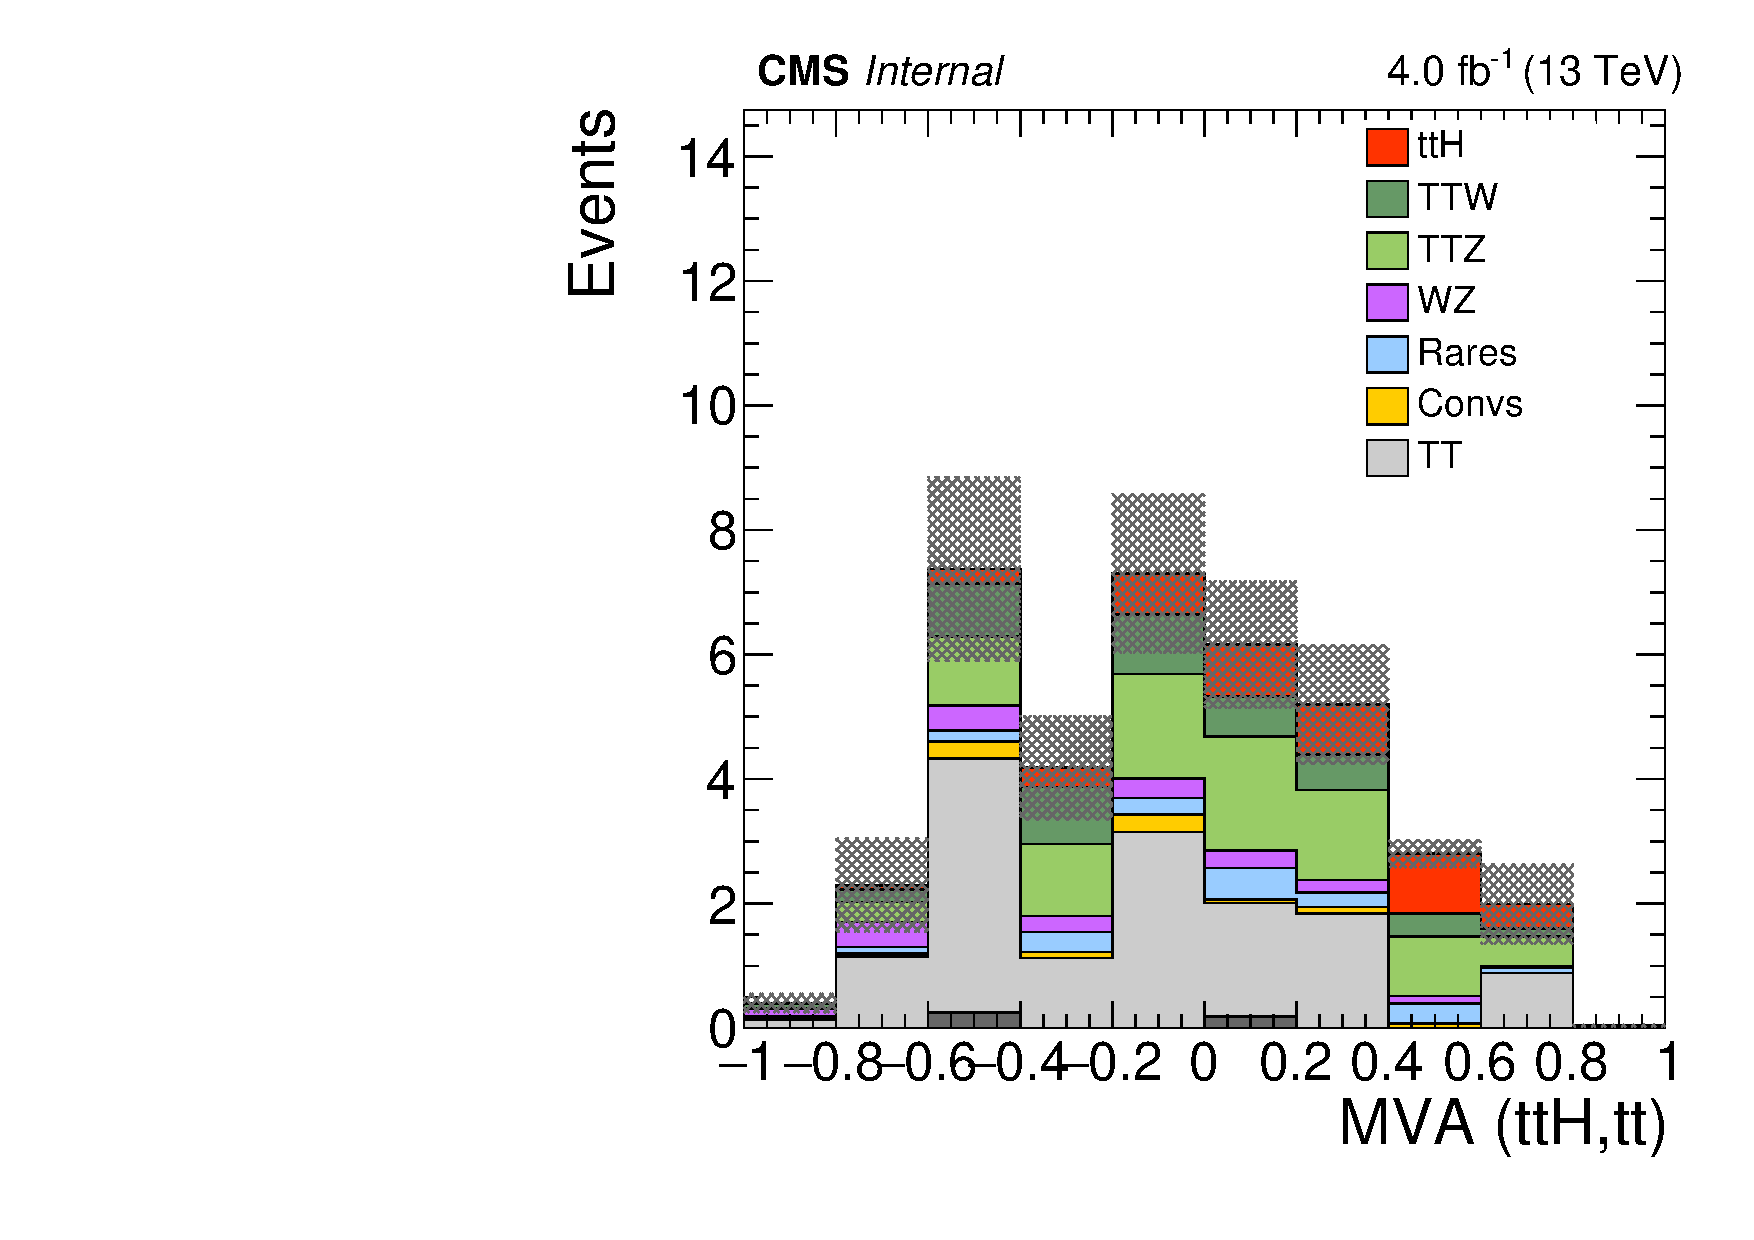
\includegraphics[width=0.35\textwidth]{plots_extraction/selection/3l_SR/kinMVA_3l_ttbar}
%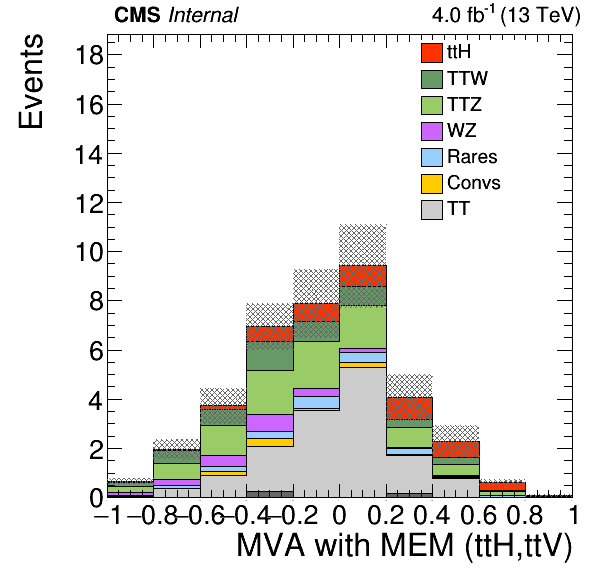
\includegraphics[width=0.35\textwidth]{plots_extraction/selection/3l_SR/kinMVA_3l_ttV_withMEM}\\
\includegraphics[width=0.35\textwidth]{plots_extraction/selection_data/3l_SR/kinMVA_3l_ttbar.pdf}
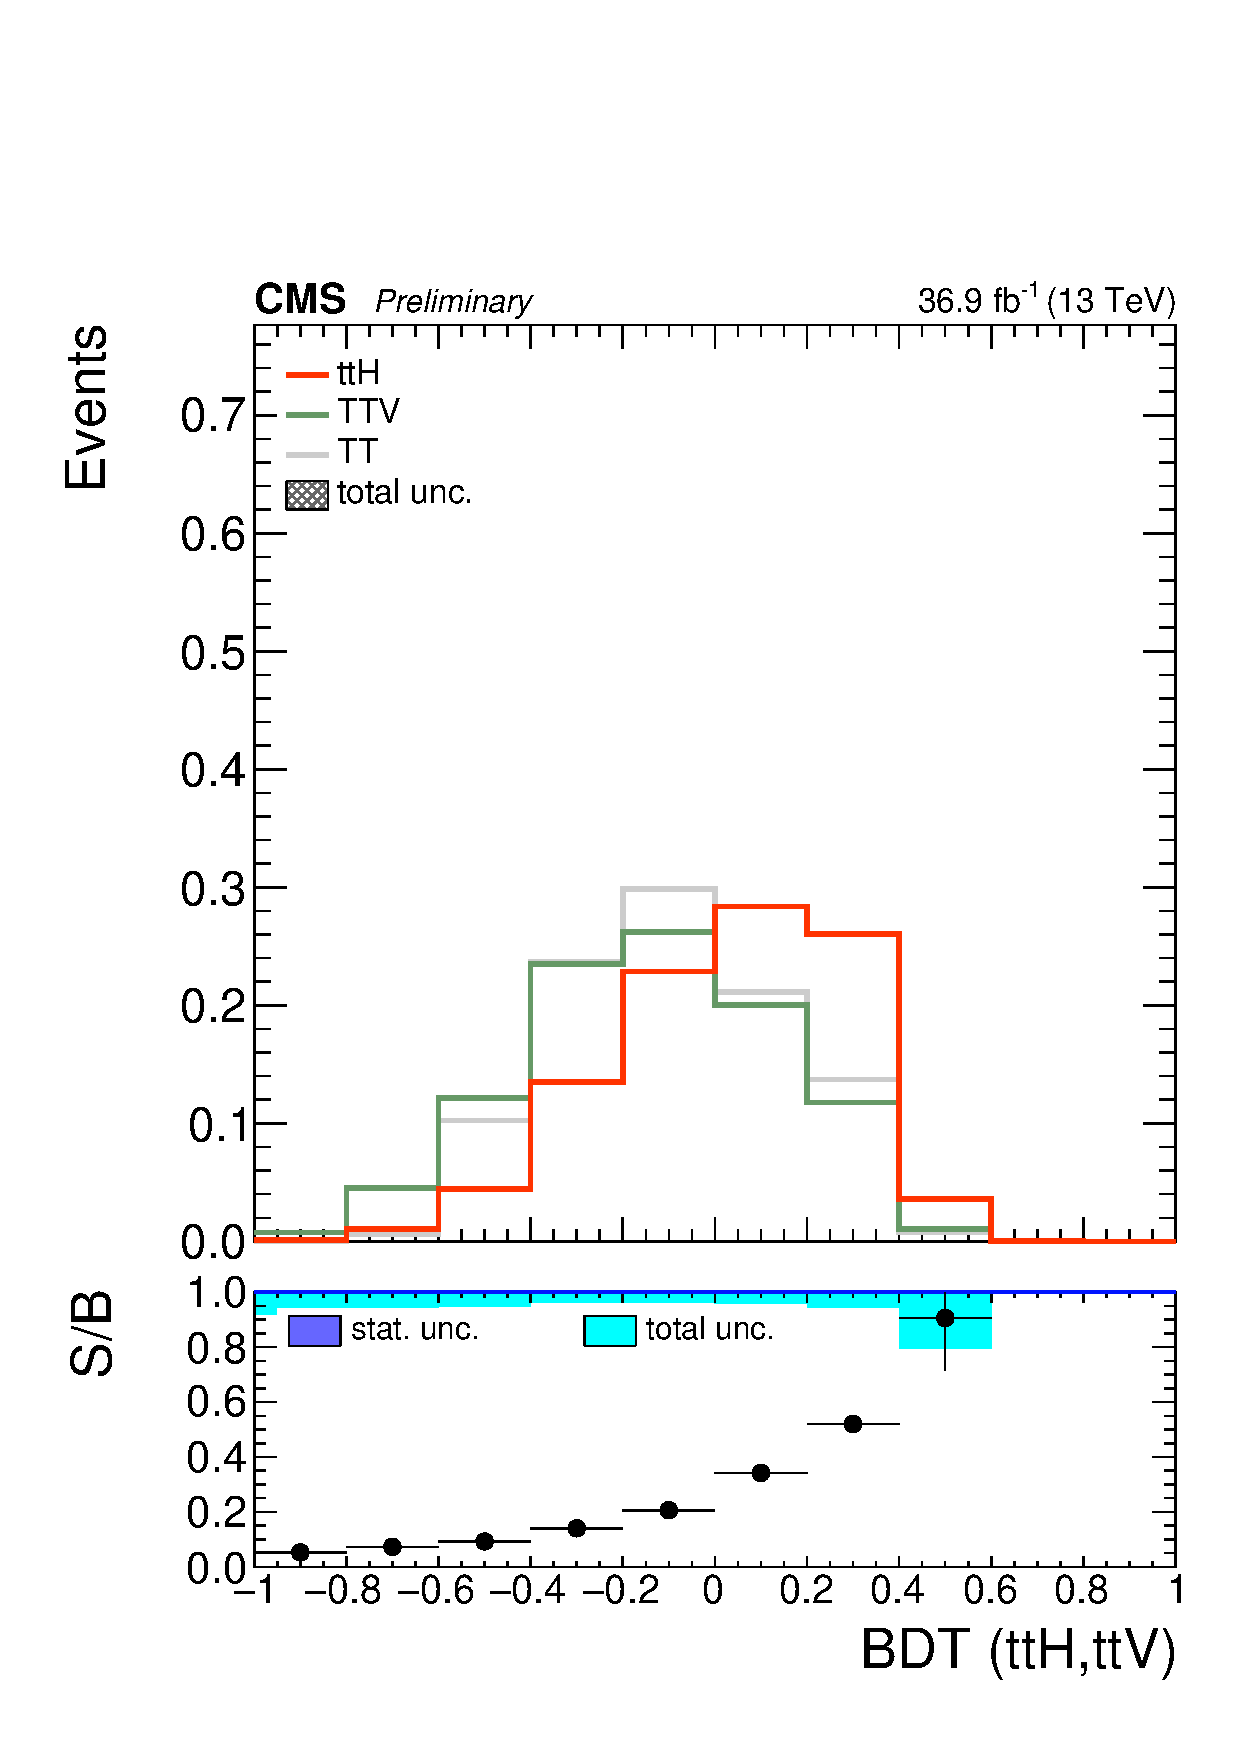
\includegraphics[width=0.35\textwidth]{plots_extraction/selection_data/3l_SR/kinMVA_3l_ttV.pdf}
\caption{Distribution of the discriminator against the ttbar (left) and ttV (right) backgrounds, in the three lepton channel, with reducible background prediction from MC (top) and from data (bottom).}
\label{fig:3l_mvaOutput}
\end{figure}

\clearpage
\subsection{2D BDT binning}\label{sec:2lss event BDT}
The two-dimensional plane spanned by the ouptut of the two BDTs is populated by signal and background events in a non-uniform way: the two-dimensional distribution of the discriminators for the ttH signal (top), and for the ttbar (bottom left) and ttV (bottom right) backgrounds, are shown in Figures~\ref{fig:2l_2dmaps} and~\ref{fig:3l_2dmaps} for the same-sign dileptonic and the multileptonic inclusive signal regions, respectively. 

\begin{figure}[htb]
	\centering
        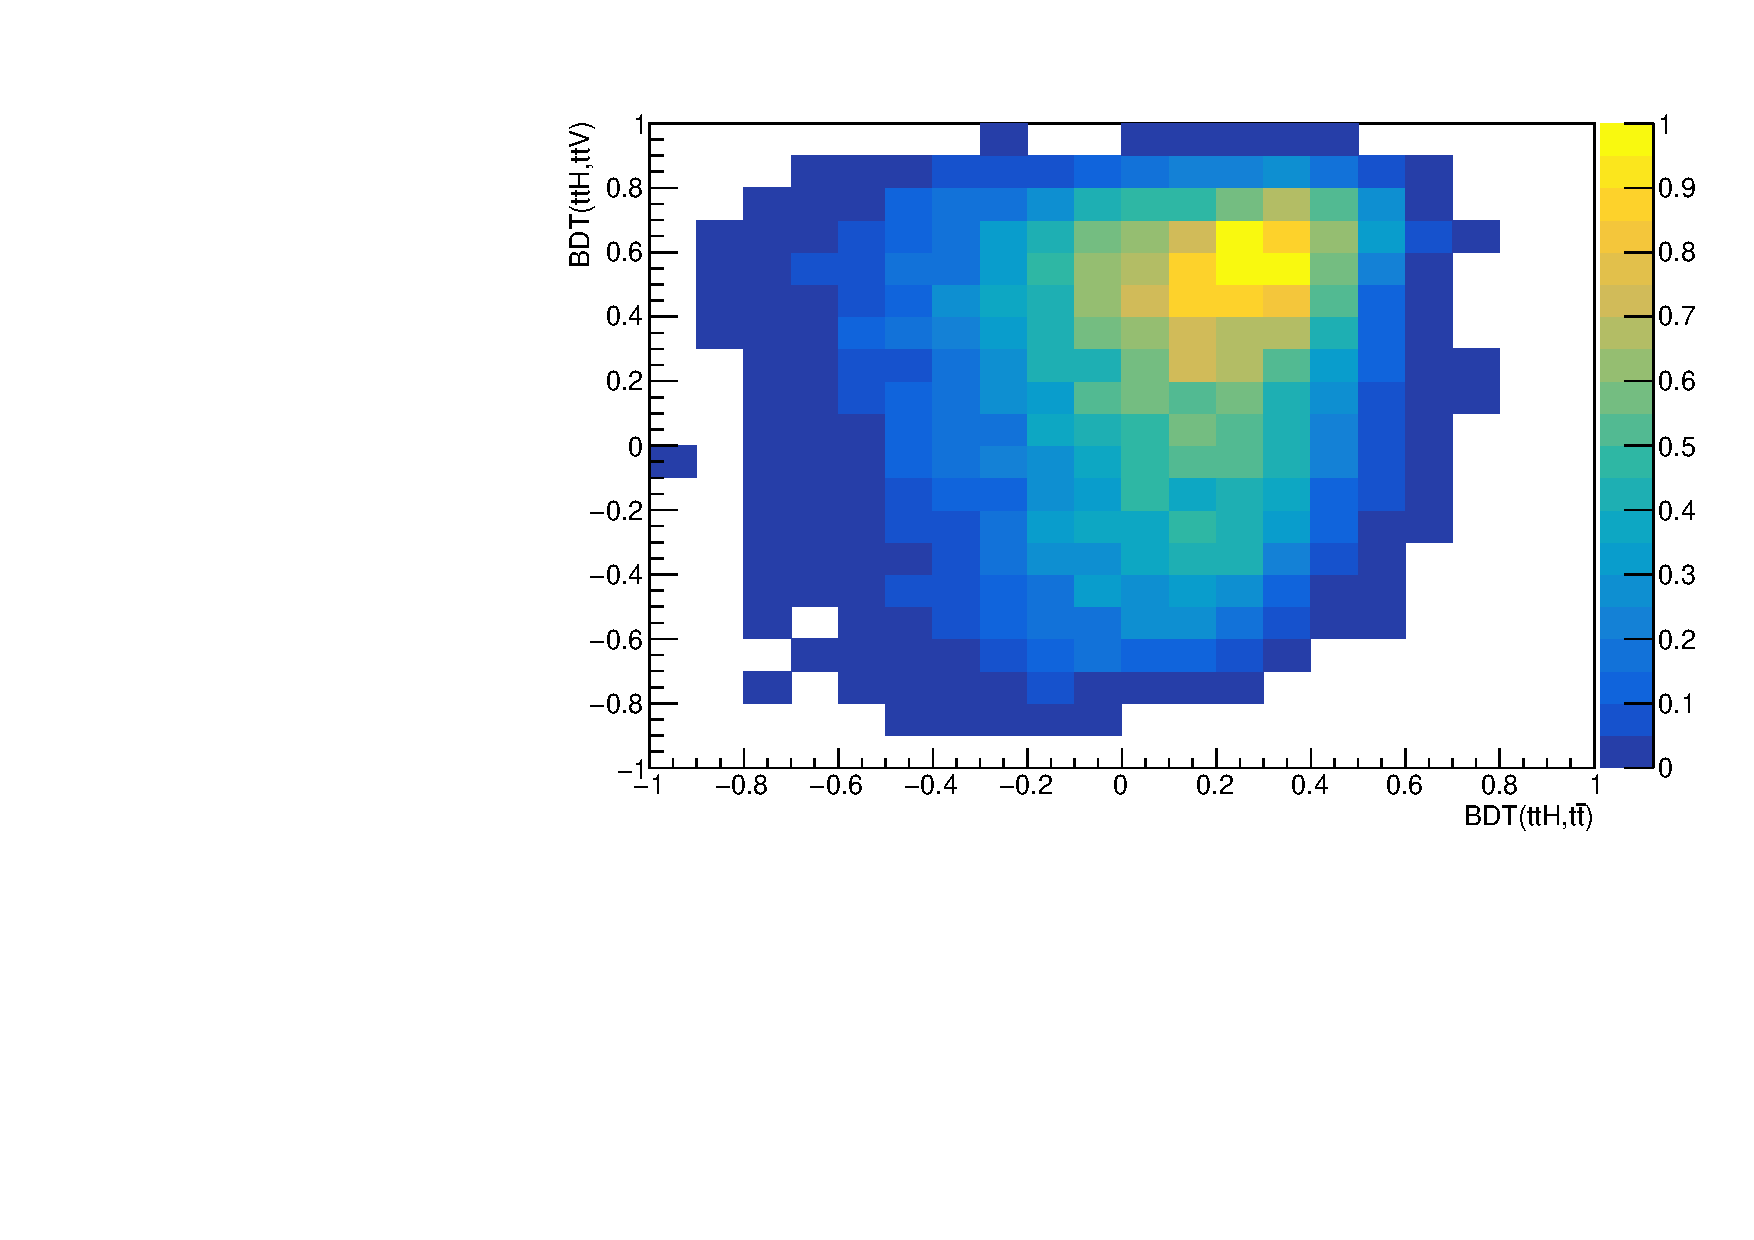
\includegraphics[width=0.35\textwidth]{plots_extraction/binning/2dmaps/tth_2l_2D}\\
        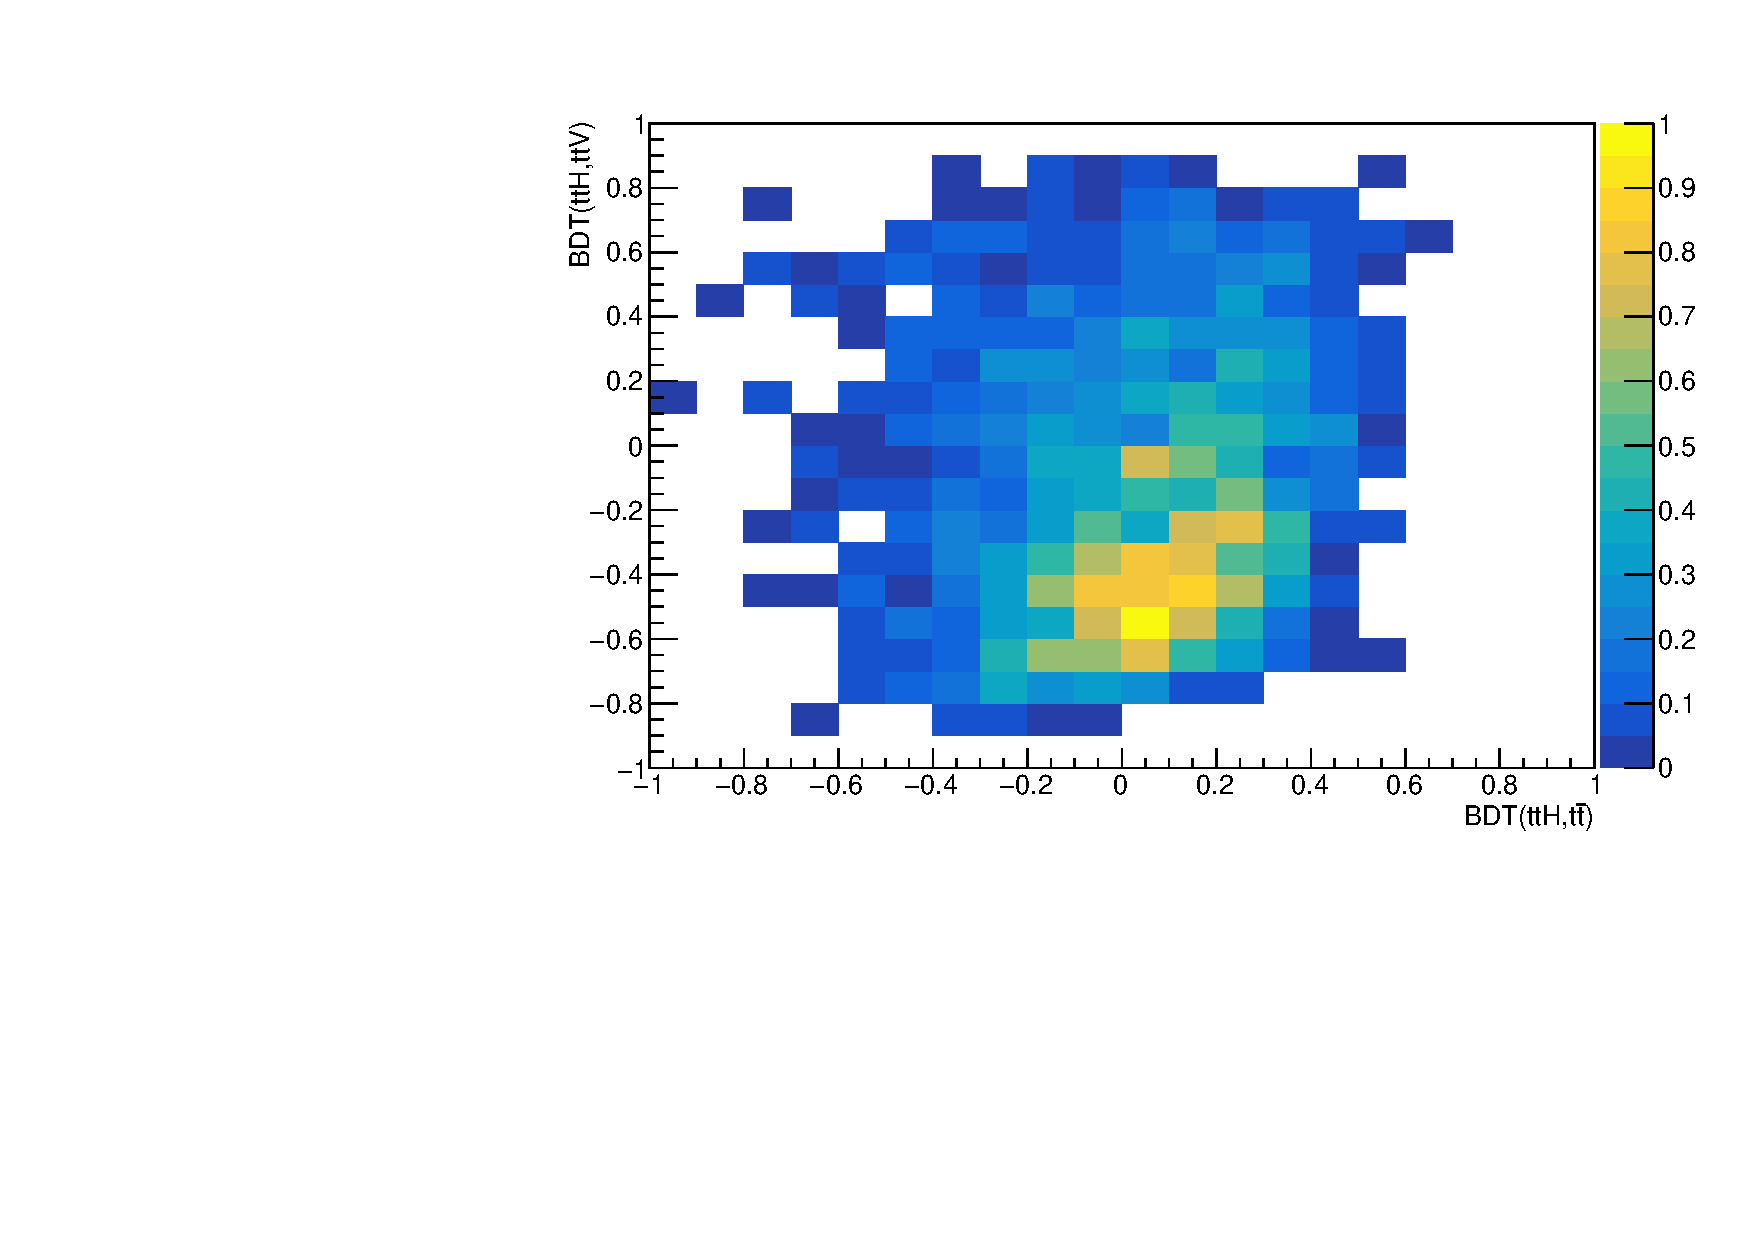
\includegraphics[width=0.35\textwidth]{plots_extraction/binning/2dmaps/tt_2l_2D}
        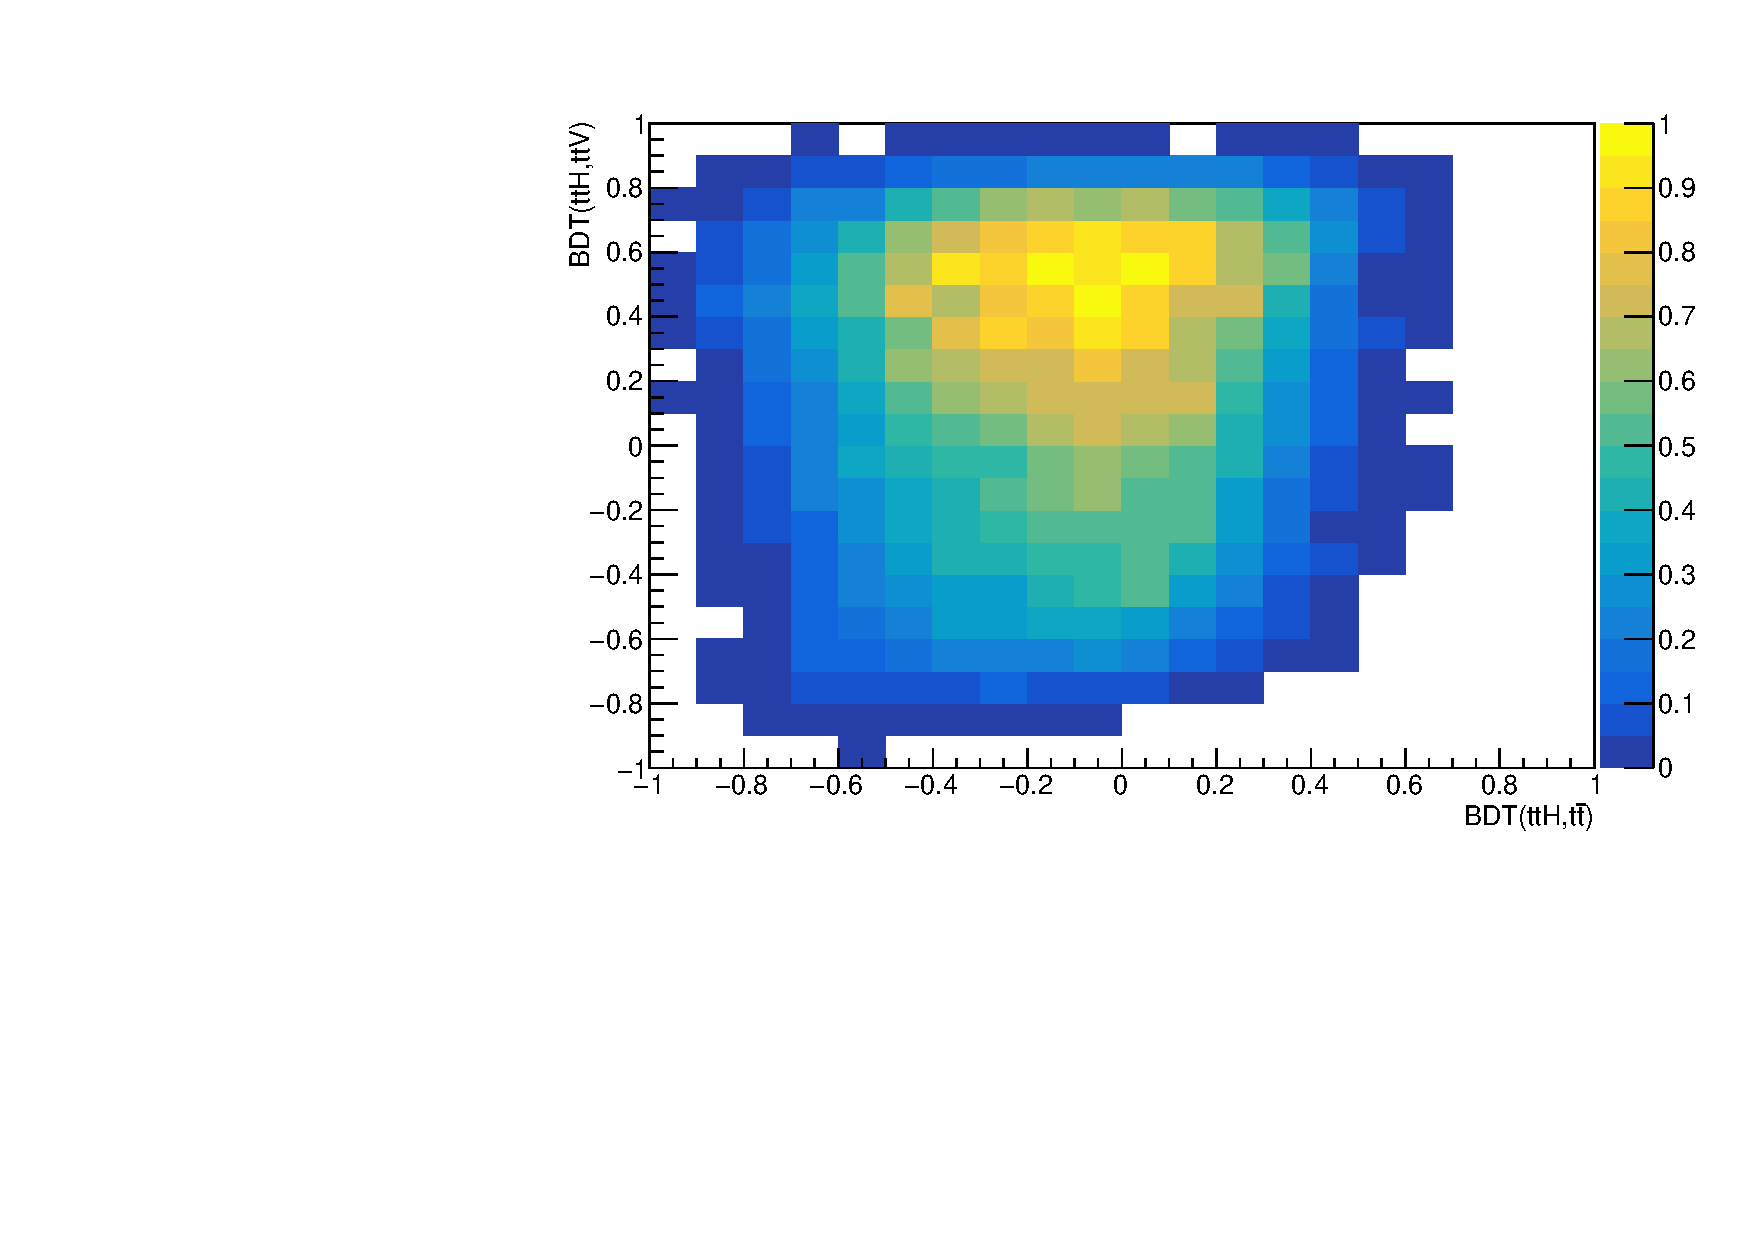
\includegraphics[width=0.35\textwidth]{plots_extraction/binning/2dmaps/ttw_2l_2D}
        \caption{Two-dimensional distribution of the discriminators for the \ttH signal (top), and for the \ttbar (bottom left) and \ttV\ (bottom right) backgrounds, in the two same sign leptons channel, estimated from MC.}
	\label{fig:2l_2dmaps}
\end{figure}

\begin{figure}[htb]
	\centering
        \includegraphics[width=0.35\textwidth]{plots_extraction/binning/2dmaps/tth_3l_2D}\\
        \includegraphics[width=0.35\textwidth]{plots_extraction/binning/2dmaps/tt_3l_2D}
        \includegraphics[width=0.35\textwidth]{plots_extraction/binning/2dmaps/ttw_3l_2D}
        \caption{Two-dimensional distribution of the discriminators for the \ttH~signal (top), and for the \ttbar~(bottom left) and \ttV~(bottom right) backgrounds, in the three lepton channel, estimated from MC.}
	\label{fig:3l_2dmaps}
\end{figure}

\begin{figure}[htb]
	\centering
        \includegraphics[width=0.35\textwidth]{plots_extraction/binning/3l/cookItUp}\\
        \caption{The discriminator of the $\mathrm{BDT(ttH,ttV)}$~classifier for simulated \ttV events, when the training is performed with or without the MEM discriminator among the input variables. A $\chi^{2}$ fit is performed, assuming linear dependence.}
	\label{fig:3l:cookItUp}
\end{figure}

The two-dimensional plane is then partitioned in several regions, depending on their different
signal or background composition, with the objective of maximizing the analysis sensitivity with the available luminosity. To do so, a method based on the likelihood ratio of signal and bakground is used.

Formally, this corresponds to building a multivariate classifier to reduce the dimensionality of the problem from two to one.

The plane is populated with events taken from simulated samples that are not used in the main analysis. Furthermore, for each simulated sample (\ttH signal, \ttbar and \ttV\ backgrounds) half of the events are used for training, and the other half are used to evaluate the performance of the classifier.

\textit{As the MEM method is vastly computer intensive, it has not been possible to compute the matrix element for the \ttbar~sample in the three leptons final state. For this reason, \ttV~events are used to assess the eventual correlation between the $\mathrm{BDT(ttH,ttV)}$ outputs obtained when training with or without the MEM discriminator among the inputs. Figure~\ref{fig:3l:cookItUp} shows the positive correlation found between the $\mathrm{BDT(ttH,ttV)}$ output in \ttV~events. A linear dependence is assumed, and under this assumption a function relating the non-MEM-trained BDT output and the MEM-trained BDT output is found via a $\chi^{2}$~fit to the \ttV~simulated events. The parameters of the fit are determined with 2--10\% accuracy, and the resulting estimator, $\hat{BDT}_{mem}(ttH,ttV) = 0.04804 + 0.6902\times BDT(ttH,ttV)_{nomem} $, is used in place of the output of the $\mathrm{BDT(ttH,ttV)}$ trained without MEM discriminator as an input. This relies on the assumption that the introduction of the MEM discriminator as an input to the $\mathrm{BDT(ttH,ttV)}$ training has the same effect in \ttbar~events as in \ttV~events. As soon as it will be possible to compute MEM for \ttbar~events, the conversion function will be removed.}

The plane, populated with training events, is binned finely, depending on the available statistics: the binning is finer ($20\times20$) for the two same sign leptons final state, and coarser ($10\times10$) for the three leptons final state. For each bin, the likelihood ratio between signal and background is computed.

In order to obtain an optimal one-dimensional classifier starting from the two-dimensional likelihood ratio distribution, an ordering criterion for the bins is devised. First the likelihood distribution for background events is obtained by assigning to each background event the likelihood ratio corresponding to the bin the event belongs to. The fine granularity of the binning ensures that this assignment is a good approximation of the true underlying likelihood function. From the distribution of the likelihood ratio for background events, the corresponding cumulative distribution is computed. A choice for the final number of bins is performed, by taking into account the available statistics in the training samples, and the quantiles of the cumulative likelihood ratio distribution for background distribution are used to divide it into the target number of final bins. The cumulative likelihood ratio distribution for background events, and its partition in quantiles, are shown in Fig.~\ref{fig:cumulative} for the two same sign leptons (left) and three leptons (right) final states respectively.

%The cumulative likelihood ratio distribution for background events, and its partition in quantiles, are shown in the left part of Fig.~\ref{fig:2l_likelihoodBinning}~and~\ref{fig:3l_likelihoodbinning}~for the two same sign leptons and three leptons (right) final states respectively.

The map between the initial and the final binning is shown in the left part of Fig.~\ref{fig:2l_likelihoodBinning}~and~\ref{fig:3l_likelihoodBinning}~for the two same sign leptons and three leptons final states respectively. Such construction guarantees that the final bins are populated by background events in an uniform way. The resulting one-dimensional distributions, obtained using the testing events, are shown in the right part of Fig.~\ref{fig:2l_likelihoodBinning}~and~\ref{fig:3l_likelihoodBinning}~for the two same sign leptons and three leptons final states respectively. The population of the background the testing distribution is not perfectly uniform in the testing sample because of statistical fluctuation of the testing and training samples. 

\begin{figure}[htb]
	\centering
        \includegraphics[width=0.35\textwidth]{plots_extraction/binning/2lss/cumulative_2lss}       
        \includegraphics[width=0.35\textwidth]{plots_extraction/binning/3l/cumulative_3l}\\
        \caption{Cumulative likelihood ratio distribution for background events for the two same sign leptons final state (left) and the three leptons final state (right), estimated from MC.}
	\label{fig:cumulative}
\end{figure}

\begin{figure}[htb]
	\centering
        \includegraphics[width=0.35\textwidth]{plots_extraction/binning/2lss/likelihoodBased_2d_2lss.png}
        \includegraphics[width=0.35\textwidth,height=0.35\textwidth]{plots_extraction/binning/2lss/likelihoodBased_1d_2lss}
        \caption{The location of the different bins in the two-dimensional plane (left), as well as the number of expected events in each bin (right) in the two same sign leptons channel, estimated from MC.}
	\label{fig:2l_likelihoodBinning}
\end{figure}


\begin{figure}[htb]
	\centering
        \includegraphics[width=0.35\textwidth]{plots_extraction/binning/3l/likelihoodBased_2d_3l.png}
        \includegraphics[width=0.35\textwidth,height=0.35\textwidth]{plots_extraction/binning/3l/likelihoodBased_1d_3l}
        \caption{The location of the different bins in the two-dimensional plane (left), as well as the number of expected events in each bin (right) in the three leptons channel, estimated from MC.}
	\label{fig:3l_likelihoodBinning}
\end{figure}

To check that the choice number of final bins in each final state is indeed suitable, an alternative method that does not require any assumption on the final number of bins is used, based on the $k$-means algorithm~\cite{MR0090073,macqueen1967} is used, yielding similar results and thus confirming the soundness of the choice of number of final bins. Such method is detailed in Appendix~\ref{sec:kmeans}.% {\it The number of bins is slightly higher in each final state because of the higher statistics samples used for this latest run. In a couple days we will provide updated plots for the appendix, using the same samples used for the likelihood ratio based method.}

%% \begin{table}[thb]
%% \centering
%% \caption{Coordinates of the bins that represent the partitioning of the 2D BDT plane.}
%% \label{tab:binning}
%% \begin{tabular}{lllllllllllllllll}
%% \hline
%%                    & bin 1 & bin 2 & bin 3 & bin 4 & bin 5 & bin 6 & bin 7\\
%% \hline
%% $2lss (\ttbar)$     & (-1.0, -0.2] & (-0.2, 0.1] & (0.1, 0.4] & (0.1, 0.4] & (0.4, 1.0] & (0.4, 1.0] & (0.4, 1.0] \\
%% $2lss (\ttV)$       & (-1.0, 1.0] & (-1.0, 1.0] & (-1.0, 0.3] & (0.3, 1.0] & (-1.0, 0.1] & (0.1, 0.4] & (0.4, 1.0]\\ \hline

%% $3\ell (\ttbar)$      & (-1.0, -0.3] & (-0.3, 0.3] & (-0.3, 0.3] & (0.3, 1.0]  & (0.3, 1.0]  & & \\
%% $3\ell (\ttV)$        & (-1.0, 1.0] & (-1.0, 0.25] & (0.25, 1.0] & (-1.0, 0.25] & (0.25, 1.0] & & \\

%% \hline
%% \end{tabular}
%% \end{table}

Figure~\ref{fig:kinMVA_binning} shows the event yield as a function of the bins defined above.

\begin{figure}[htb]
	\centering
\includegraphics[width=0.35\textwidth]{plots_extraction/selection_data/2lss_SR/kinMVA_2lss_bins8_withBDTv8_withHj_ourBinning.pdf}
\includegraphics[width=0.35\textwidth]{plots_extraction/selection_data/3l_SR/kinMVA_3l_bins5_ourBinning.pdf}
	\caption{Binned distributions of the pair of discriminators in 2lss (left) and 3l (right) channels.}
	\label{fig:kinMVA_binning}
\end{figure}

%\begin{figure}[htb]
%	\centering
%\includegraphics[width=0.35\textwidth]{plots_extraction/selection_data/2lss_SR/postfit_kinMVA_2lss_bins}
%\includegraphics[width=0.35\textwidth]{plots_extraction/selection_data/3l_SR/postfit_kinMVA_3l_bins}
%	\caption{\textbf{Post-fit} binned distributions of the pair of discriminators in 2lss (left) and 3l (right) channels.}
%	\label{fig:kinMVA_binning_postfit}
%\end{figure}


%\begin{figure}[htb]
%	\centering
%\includegraphics[width=0.4\textwidth]{plots_extraction/selection_data/2lss_SR/kinMVA_2lss_catbinIndex}
%\includegraphics[width=0.4\textwidth]{plots_extraction/selection_data/3l_SR/kinMVA_3l_catbinIndex}
%	\caption{Splitting in categories and BDT bins for the 2lss and 3l channels.}
%	\label{fig:catbinsplitting}
%\end{figure}

%% Don't forget to also reference it in the text
%% add when MEM weights available\begin{figure}[htb]
%% add when MEM weights available	\centering
%% add when MEM weights available\includegraphics[width=0.32\textwidth]{plots_extraction/selection_data/3l_SR/kinMVA_input_MEM_TTH}
%% add when MEM weights available\includegraphics[width=0.32\textwidth]{plots_extraction/selection_data/3l_SR/kinMVA_input_MEM_TTW}
%% add when MEM weights available\includegraphics[width=0.32\textwidth]{plots_extraction/selection_data/3l_SR/kinMVA_input_MEM_TTZ}
%% add when MEM weights available	\caption{MEM weights for ttH, ttW and ttZ hypotheses in the 3l channel.}
%% add when MEM weights available	\label{fig:memweights}
%% add when MEM weights available\end{figure}

\subsection{Event subcategories}

Events are further split into lepton flavours: two electrons, two muons and electron and muon. These three categories, except
the two electrons, are further divided according to the presence (or absence) of two medium tagged b-jets, the b-tight (b-loose) categories.

The events with at least three leptons are only separated into the b-tight and b-loose categories.

Finally, to exploit the charge asymmetry present in several backgrounds (ttW, WZ, single top and W+jets), but not present in ttH,
events in each of the categories described above are further categorized by the positive or negative sum of the lepton charges. The
summary of all event categories is summarized in Figure~\ref{fig:category_table}.

\begin{figure}[htb]
	\centering
\includegraphics[width=0.70\textwidth]{plots_extraction/categories/categories_notau.png}
	\caption{Diagram of all event categories in the analysis. Categories are based on lepton multiplicity and flavor,
         b-jet composition, and the sign of the sum of the lepton charges.}
	\label{fig:category_table}
\end{figure}

\begin{figure}[htb]
	\centering
\includegraphics[width=0.4\textwidth]{plots_extraction/selection_data/2lss_SR/2lep_catIndex.pdf}
\includegraphics[width=0.4\textwidth]{plots_extraction/selection_data/3l_SR/3lep_catIndex.pdf}
	\caption{Splitting in categories for the 2lss (left) and 3l (right) channels.}
	\label{fig:catsplitting}
\end{figure}




%\begin{figure}[htb]
%	\centering
%\includegraphics[width=0.4\textwidth]{plots_extraction/categories/kinMVA_2lss_bins7}
%\includegraphics[width=0.4\textwidth]{plots_extraction/categories/kinMVA_3l_bins5_withMEM}
%	\caption{Decay composition of the ttH signal in 2lss (left) and 3l (right) channels.
%\textit{We specify that all the plots related to MEM are still the ones produced during the ICHEP compaing and the MEM is currently not included in the results, altough we are currently reprocessing the MEM technique with the full 2016 data and plan to include it in the analysis.}
%}
%	\label{fig:splitting}
%\end{figure}
%
